\documentclass[t,12pt]{beamer}

\mode<presentation>
\usetheme{NCSUstat}
%% \setbeamercovered{transparent}
\usepackage[english]{babel}
\usepackage[latin1]{inputenc}
\usepackage{times}
\usepackage[T1]{fontenc}
\usepackage{booktabs}
\usepackage{amsmath}
\usepackage{amssymb}
\usepackage{graphicx}
\usepackage{subfig}
\usepackage{multirow}

\graphicspath{{../images/}}

\let\bld\boldsymbol

\usepackage[backend=bibtex]{biblatex}
\bibliography{AdityaKashi-MSdefense}

% for contents slides
\AtBeginSection{
	\begin{frame}{Table of Contents}
		\tableofcontents[currentsection]
	\end{frame}
}

\title[Mesh movement and curved mesh generation] % (optional, use only with long paper titles)
{Techniques for Mesh Movement and Curved Mesh Generation}
\subtitle{for Computational Fluid Dynamics} % (optional)
\author[] % (optional, use only with lots of authors)
{Aditya Kashi}
\institute[NCSU]
{
  Department of Mechanical and Aerospace Engineering,\\
  North Carolina State University
}
\footlineupper{\insertshorttitle}
\footlinelower{\copyright{} 2016 by Aditya Kashi}
\subject{Computational Fluid Dynamics}


\date{April 27, 2016} %% uncomment to leave out the date, or to use a specific date

%%%%%%%%%%%%%%%%%%%%%%%%%%%%%%%%%%%%%%%%%%%%%%%%%%%%%%%%%%%%%%%%%%%%%%
\begin{document}

\begin{frame}
  \titlepage
\end{frame}

%%%%%%%%%%%%%%%%%%%%%%%%%%%%%%%%%%%%%%%%%%%%%%%%%%%%%%%%%%%%%%%%%%%%%%
\section{Section I : Introduction}

\subsection{Need for mesh movement}

\begin{frame}
  \frametitle{Why mesh movement?}
  \begin{block}{Mesh movement is useful in several areas of CFD}
	  \begin{itemize}
	  	\item aeroelasticity, and fluid-structure interaction in general
	  	\item shape optimization
	  	\item generation of curved meshes for spatially high-order discretizations
	  	\item others
	  \end{itemize}
  \end{block}
\end{frame}

\begin{frame}{Fluid-Structure Interaction}
	\begin{itemize}
		\item For a body-fitted grid, robust mesh-movement is required to maintain validity and quality of the mesh after imposing motion of the structural domain \footfullcite{appl:fsi}.
		\item Immersed boundary methods can also be used; both have advantages and disadvantages \footfullcite{appl:fsireview}.
	\end{itemize}
\end{frame}

\begin{frame}{Shape optimization}
	\begin{figure}
		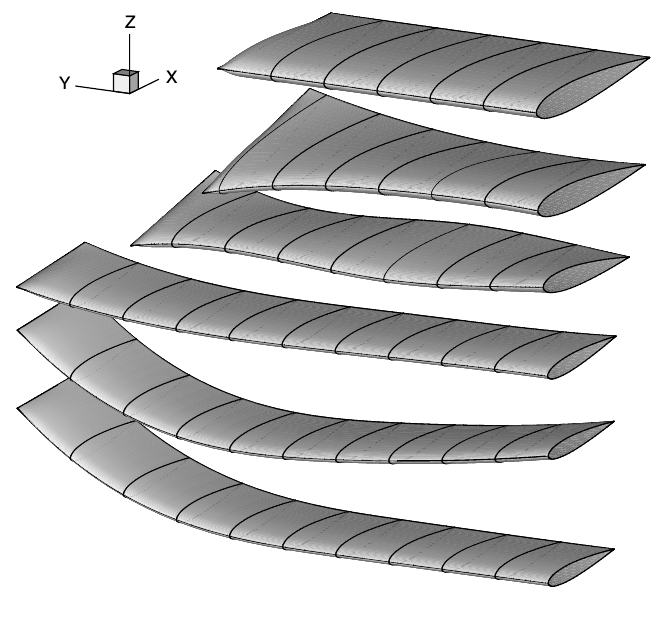
\includegraphics[scale=0.2]{ppt-illus-shapeoptimization}
		\caption{Convergence history of lift-constrained drag minimization }
	\end{figure}
	\footfullcite{appl:opt2}
\end{frame}

\subsection{Need for curved meshes}
\begin{frame}{High-order methods}
\begin{itemize}
  \item According to Wang, Fidkowski \emph{et. al.} \footfullcite{highorder}, spatially high-order methods perform better than prevailing second order methods for some kinds of simulations considering CPU time taken to achieve a given error level.
  \item One area of challenge they mention is generation of high-order meshes.
\end{itemize}
\begin{figure}
		\centering
		\subfloat{
			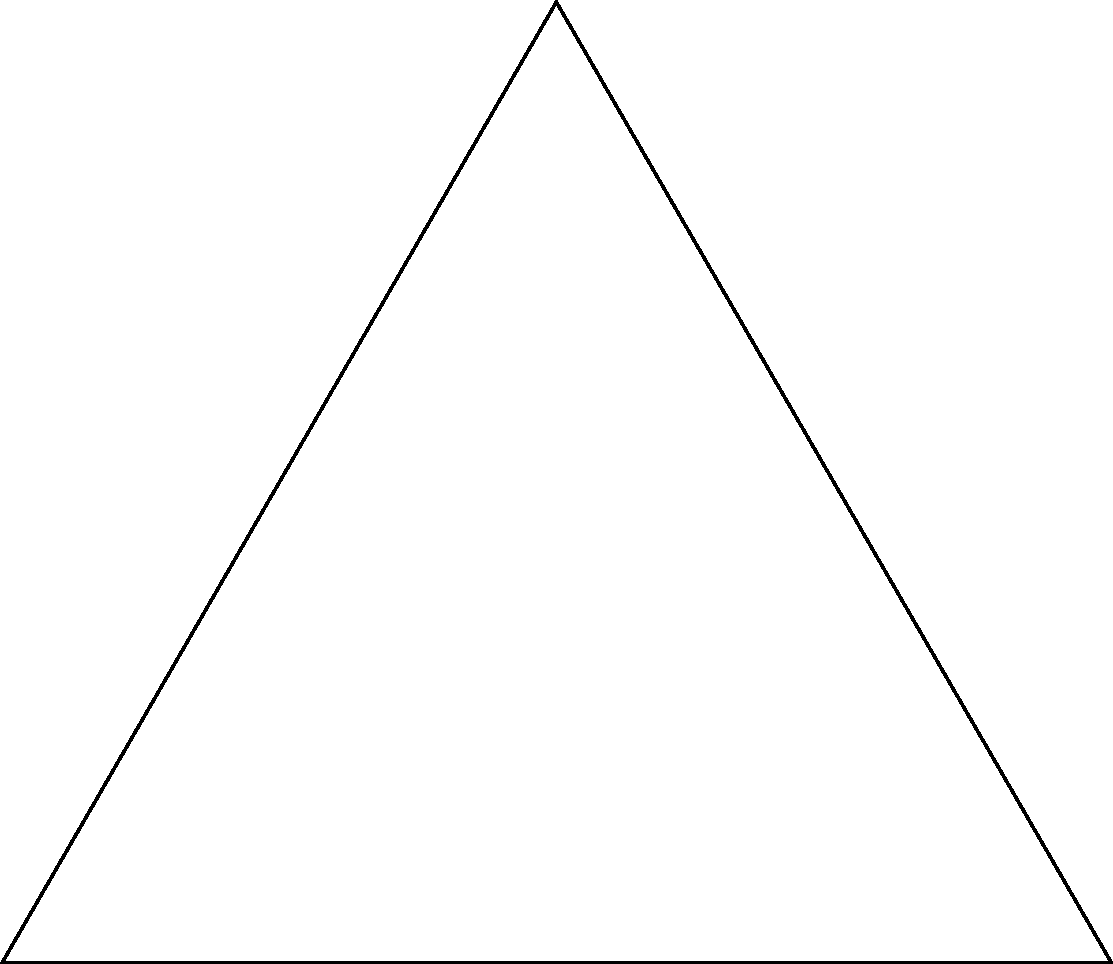
\includegraphics[scale=0.07]{tri_ideal}
		}
		\hspace{0.2in}
		\subfloat{
			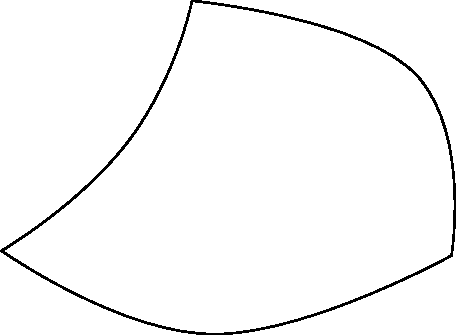
\includegraphics[scale=0.2]{tri_curved}
		}
		\caption{Regular linear triangle (left) and high-order curved `triangle' (right)}
		\label{fig:curvedelement}
\end{figure}
\end{frame}

\begin{frame}{The need for curved meshes}
 \begin{figure}
 	\centering
 	\subfloat{
 		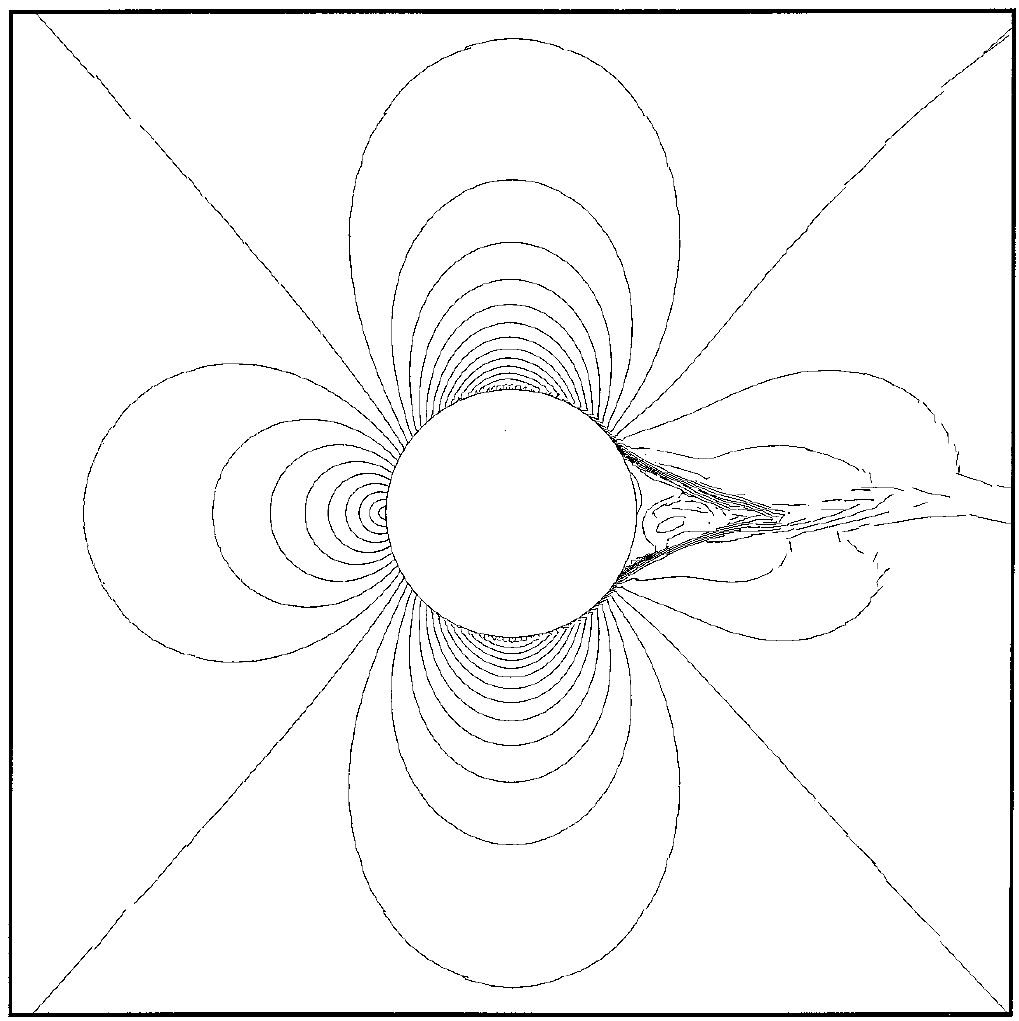
\includegraphics[scale=0.12]{bassi-linear}
 	}
 	\subfloat{
 		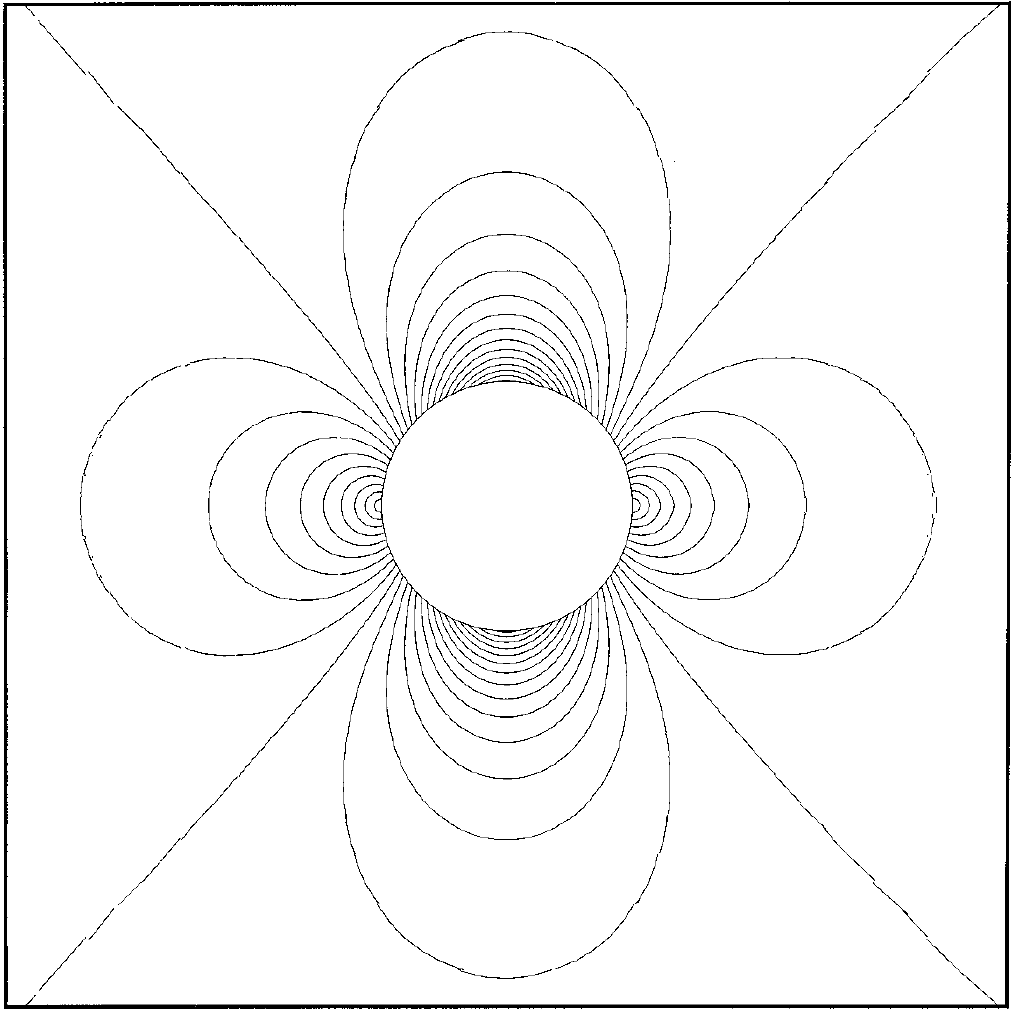
\includegraphics[scale=0.12]{bassi-q2}
 	}
 	\caption{Inviscid subsonic flow over a cylinder; left: DGP1 solution with regular linear mesh, right: DGP1 solution with quadratic (`Q2') mesh \footfullcite{appl:dgeuler}}
 	\label{fig:bassi}
 \end{figure}
\end{frame}

\begin{frame}{The need for curved meshes}
Even in less extreme cases, curved meshes are required to obtain design (p+1) order of accuracy for high-order methods such as discontinuous Galerkin methods \footfullcite{curve:geomacc}.
\end{frame}

%%%%%%%%%%%%%%%%%%%%%%%%%%%%%%%%%%%%%%%%%%%%%%%%%%%%%%%%%%%%%%%%%%%%%%
\section{Section II : Mesh movement}

\begin{frame}{Introduction}
The problem is to move the interior nodes of a mesh when a given displacement is imposed on the boundary.
\begin{itemize}
	\item At the very least: mesh elements should not get invalidated.
	\item Mesh elements should not suffer much deterioration in quality.
	\item The technique should be computationally inexpensive.
\end{itemize}
\end{frame}

\begin{frame}{Element validity for finite element methods}
Since we cannot integrate over arbitrary sets, physical elements are mapped to a reference element using a geometric mapping.
\begin{figure}
	\includegraphics[scale=0.3]{geommapping}
	\caption{Geometric mapping between reference element $S$ (left) and physical element $\Omega$ (right)}
\end{figure}
Change of variables theorem: if the mapping $\bld{f}:S\rightarrow\Omega$ is bijective and differentiable, we can integrate over the reference element instead. This requires the Jacobian of $\bld{f}$ to be nonsingular throughout the element.
\end{frame}

\subsection{Review of methods}

\begin{frame}{Types of methods}
Many mesh-movement methods for unstructured meshes can be found in literature. They can be broadly classified into two types.
\vspace{0.2in}
\begin{itemize}
	\item Elasticity-based methods
	\item Interpolation methods
\end{itemize}
\vspace{0.2in}
Combination of these with each other and with other techniques such as topological (connectivity) smoothing are also used \footfullcite{mm:alauzet}.
\end{frame}

\begin{frame}{Lineal spring analogy}
	Every mesh edge is treated as a linear spring in each coordinate direction \footfullcite{mm:batina}.
	 \begin{equation}
	 \sum_j k_{ij}(\Delta \mathbf{r}_i - \Delta \mathbf{r}_j) = \mathbf{0} \quad \forall i
	 \label{spring}
	 \end{equation}
	 where $i$ ranges over all nodes, $j$ ranges over points surrounding node $i$ and $\Delta \mathbf{r}_i$ is the displacement of node $i$.
	 $k_{ij}$ is the stiffness of the spring between nodes $i$ and $j$, which can be taken as
	 \begin{equation}
	 k_{ij} = \frac{1}{||\mathbf{r}_i - \mathbf{r}_j||}.
	 \end{equation}
\end{frame}
\begin{frame}{Lineal spring analogy}
	\vspace{0.5in}
	This scheme requires the solution of $n_{dim}$ linear systems,
	
	each of size $N_n$ (the number of mesh nodes).
\end{frame}

\begin{frame}{Torsional springs}
The lineal spring analogy fails for large deformations or stretched elements. Farhat \emph{et. al.} came up with a more robust scheme, which is also a spring analogy \footfullcite{mm:torsionsprings}.

They introduce two improvements over Batina's model.
\begin{itemize}
	\item The model is closer to a structural analogy in that the displacements in each coordinate direction are coupled.
	\item `Torsional springs' are introduced at each node in each element. These are designed to prevent edges collapsing into each other due to rotational motion.
\end{itemize}
\end{frame}

\begin{frame}{Torsional springs}
The stiffness of the torsional springs at a node in an element is inversely related to the node angle in that element.
 \begin{figure}
 	\centering
 	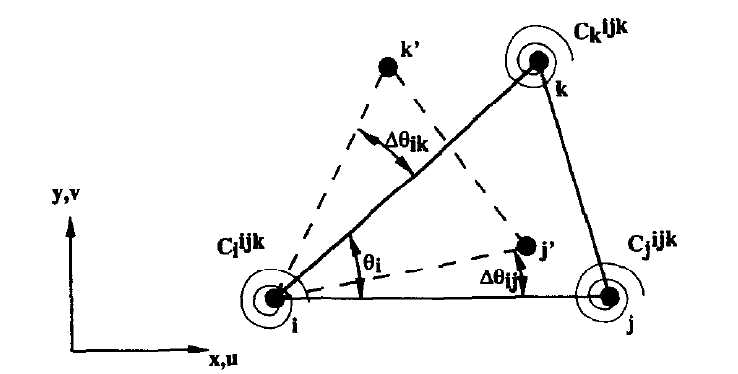
\includegraphics[scale=0.25]{torsionspring}
 	\caption{Movement of an element in torsion spring analogy}
 	\label{fig:torsion}
 \end{figure}
 A coupled SPD system of $n_{dim} N_n$ equations must be solved.
\end{frame}

\begin{frame}{Linear elasticity}
  The mesh is assumed to model a deformable solid body, which is then deformed according to the equations of solid mechanics, that is, linear or non-linear elasticity.
  
  The simplest approach is linear elasticity.
  \begin{equation}
  \nabla \cdot \bld{\sigma}  = \mathbf{0} \quad \text{in} \, \Omega
  \end{equation}
  \begin{equation}
  \bld{\sigma} = 2\mu\bld{\epsilon} + \lambda (\mathrm{tr}\boldsymbol{\epsilon}) \bld{I}
  \label{linelast:constt}
  \end{equation}
  \begin{equation}
  \bld{\epsilon} = \frac12 (\nabla\bld{u}+\nabla\bld{u}^T)
  \label{linelast:strain}
  \end{equation}
  \begin{equation}
  \bld{u} = \bld{u}_b \quad \text{on} \, \partial\Omega
  \end{equation}
  Implemented using a standard continuous finite element method.
\end{frame}

\begin{frame}{Stiffened Linear elasticity}
	\begin{itemize}
	\item The linear elasticity scheme is often modified by `stiffening' the mesh appropriately. 
	\item We attain some control over the propagation of deformation into the interior of the mesh, as done, for instance, by Stein \emph{et. al.} \footfullcite{mm:fsielast}.
	\item The material is stiffened based on the determinant of the local Jacobian matrix of the reference-to-physical mapping; i.e., smaller elements are stiffer than larger ones.
	\end{itemize}
\end{frame}

\begin{frame}{Elasticity-based methods}
\begin{itemize}
	\item Advantages: stiffened linear elasticity is found to be robust
	\item Disadvantage: expensive!
	\item Also, implementation is dependent on element type and spatial dimension.
\end{itemize}
\end{frame}

\begin{frame}{Delaunay graph mapping (DGM)}
Interpolation by barycentric coordinates (volume ratios) in a `background' simplicial mesh.
 \begin{figure}
 	\centering
 	\subfloat{
 		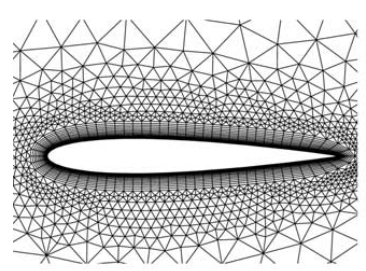
\includegraphics[scale=0.25]{dgm-mesh}
 	}
 	\subfloat{
 		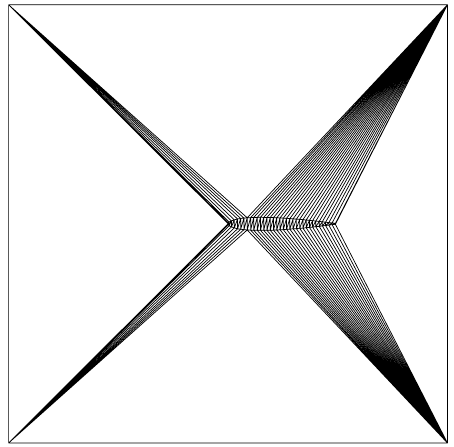
\includegraphics[scale=0.2]{dgm-dg}
 	}
 	\subfloat{
 		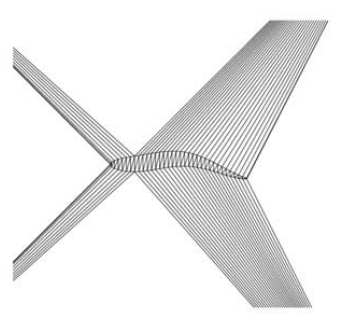
\includegraphics[scale=0.25]{dgm-moveddg}
 	}
 	\subfloat{
 		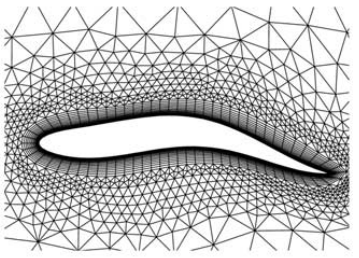
\includegraphics[scale=0.25]{dgm-movedmesh}
 	}
 	\caption{The DGM process (from left to right): original mesh, Delaunay graph, deformed Delaunay graph, deformed mesh (ref: \footfullcite{mm:dgm})}
 	\label{fig:dgmprocess}
 \end{figure}
\end{frame}

\begin{frame}{Radial basis function (RBF) interpolation}
Considering $n_b$ boundary points in the mesh, we express the displacement at any point in the mesh as \footfullcite{mm:rbf}
\begin{equation}
\mathbf{s}(\mathbf{x}) = \sum_{j=1}^{n_b} \mathbf{a}_j \phi(\lVert\mathbf{x} - \mathbf{x}_{bj}\rVert_2)
\label{eqn:rbf}
\end{equation}
$\phi$ is a radial basis function. As a function of $\bld{x}$, it is radially symmetric about the origin.
\end{frame}

\begin{frame}{RBF interpolation}
Since we know the displacements of the boundary nodes, we can solve for the coefficients $\mathbf{a}_j$ using
\begin{equation}
\mathbf{s}(\mathbf{x}_{ib}) = \sum_{j=1}^{n_b} \mathbf{a}_j \phi(\lVert\mathbf{x}_{bi} - \mathbf{x}_{bj}\rVert_2).
\end{equation}
In each coordinate direction $k$, this leads to a system of $n_b$ equations in $n_b$ unknowns:
\begin{equation}
\mathbf{A}\mathbf{a}_k = \mathbf{s}_k
\label{eqn:rbf_system}
\end{equation}
where $\bld{A}_{ij} = \phi(\lVert\mathbf{x}_{bi} - \mathbf{x}_{bj}\rVert_2)$.
\end{frame}

\begin{frame}{RBF interpolation}
The quality of the final mesh depends on which RBF is used. We use Wendland's $C^2$ function \footfullcite{rbf:errorwendland}
\begin{equation}
\phi(x) = 
\begin{cases}
\left(1-\frac{x}{r_s}\right)^4\left(4\frac{x}{r_s} + 1\right) & x < r_s \\
0 & x \geq r_s
\end{cases}
\end{equation}
$r_s$ is a real number called the `support radius'.
\begin{itemize}
	\item Compact support - leads to sparse LHS
	\item Positive definite - systems can (usually) be solved quickly
	\item $C^2$ - smooth mesh movement
\end{itemize}
\end{frame}

\begin{frame}{RBF interpolation on a Delaunay Graph (DGRBF)}
Wang \emph{et. al.} \footfullcite{mm:dgrbf} interpolate the displacements over each Delaunay graph element  using RBFs instead of barycentric coordinates.
The displacement of a node with initial position $\bld{x}$ is given by
\begin{equation}
\mathbf{s}(\mathbf{x}) = \sum_{j=1}^{n_t} \mathbf{a}_j \phi(\lVert\mathbf{x} - \mathbf{x}_{tj}\rVert_2)
\label{eqn:dgrbf}
\end{equation}
where $\bld{x}_{tj}$ are positions of nodes of the Delaunay simplex that contains the node, $n_t$ is the number of nodes in that simplex (3 in 2D and 4 in 3D). 
\end{frame}

\begin{frame}{DGRBF}
We need to solve for the $\bld{a}_j$, the RBF coefficients, by solving a $3 \times 3$ system in 2D or a $4 \times 4$ system in 3D, in each Delaunay element.
\begin{equation}
\mathbf{s}(\mathbf{x}_{ti}) = \sum_{j=1}^{n_t} \mathbf{a}_j \phi(\lVert\mathbf{x}_{ti} - \mathbf{x}_{tj}\rVert_2).
\label{eqn:dgrbfsys}
\end{equation}
This is more robust than DGM, but not as robust as RBF for large complex deformations.
\end{frame}

\begin{frame}{DGRBF with angle interpolation - `DGRBF2'}
For large rotational deformation, Wang \emph{et. al.} interpolate \emph{rotation angles} from the boundary to the interior nodes.

If $\bld{s}$ is the rotation angle instead of displacement, we get DGRBF2.

Can recover displacements using the usual rotation transformations.
\begin{exampleblock}{In 2D}
 \begin{align}
 x_{new} &= (x-x_0)\cos a_z - (y-y_0)\sin a_z + x_0 \\
 y_{new} &= (x-x_0)\sin a_z + (y-y_0)\cos a_z + y_0
 \end{align}
\end{exampleblock}
But this is difficult for general movement.
\end{frame}

\subsection{Large rotation in inviscid mesh}

\begin{frame}{Large rotation case 1}
We first present visual results of large rotation for an inviscid flow mesh of a 3-component airfoil. The flap is rotated while keeping the rest of the boundary fixed.
\begin{figure}
	\centering
	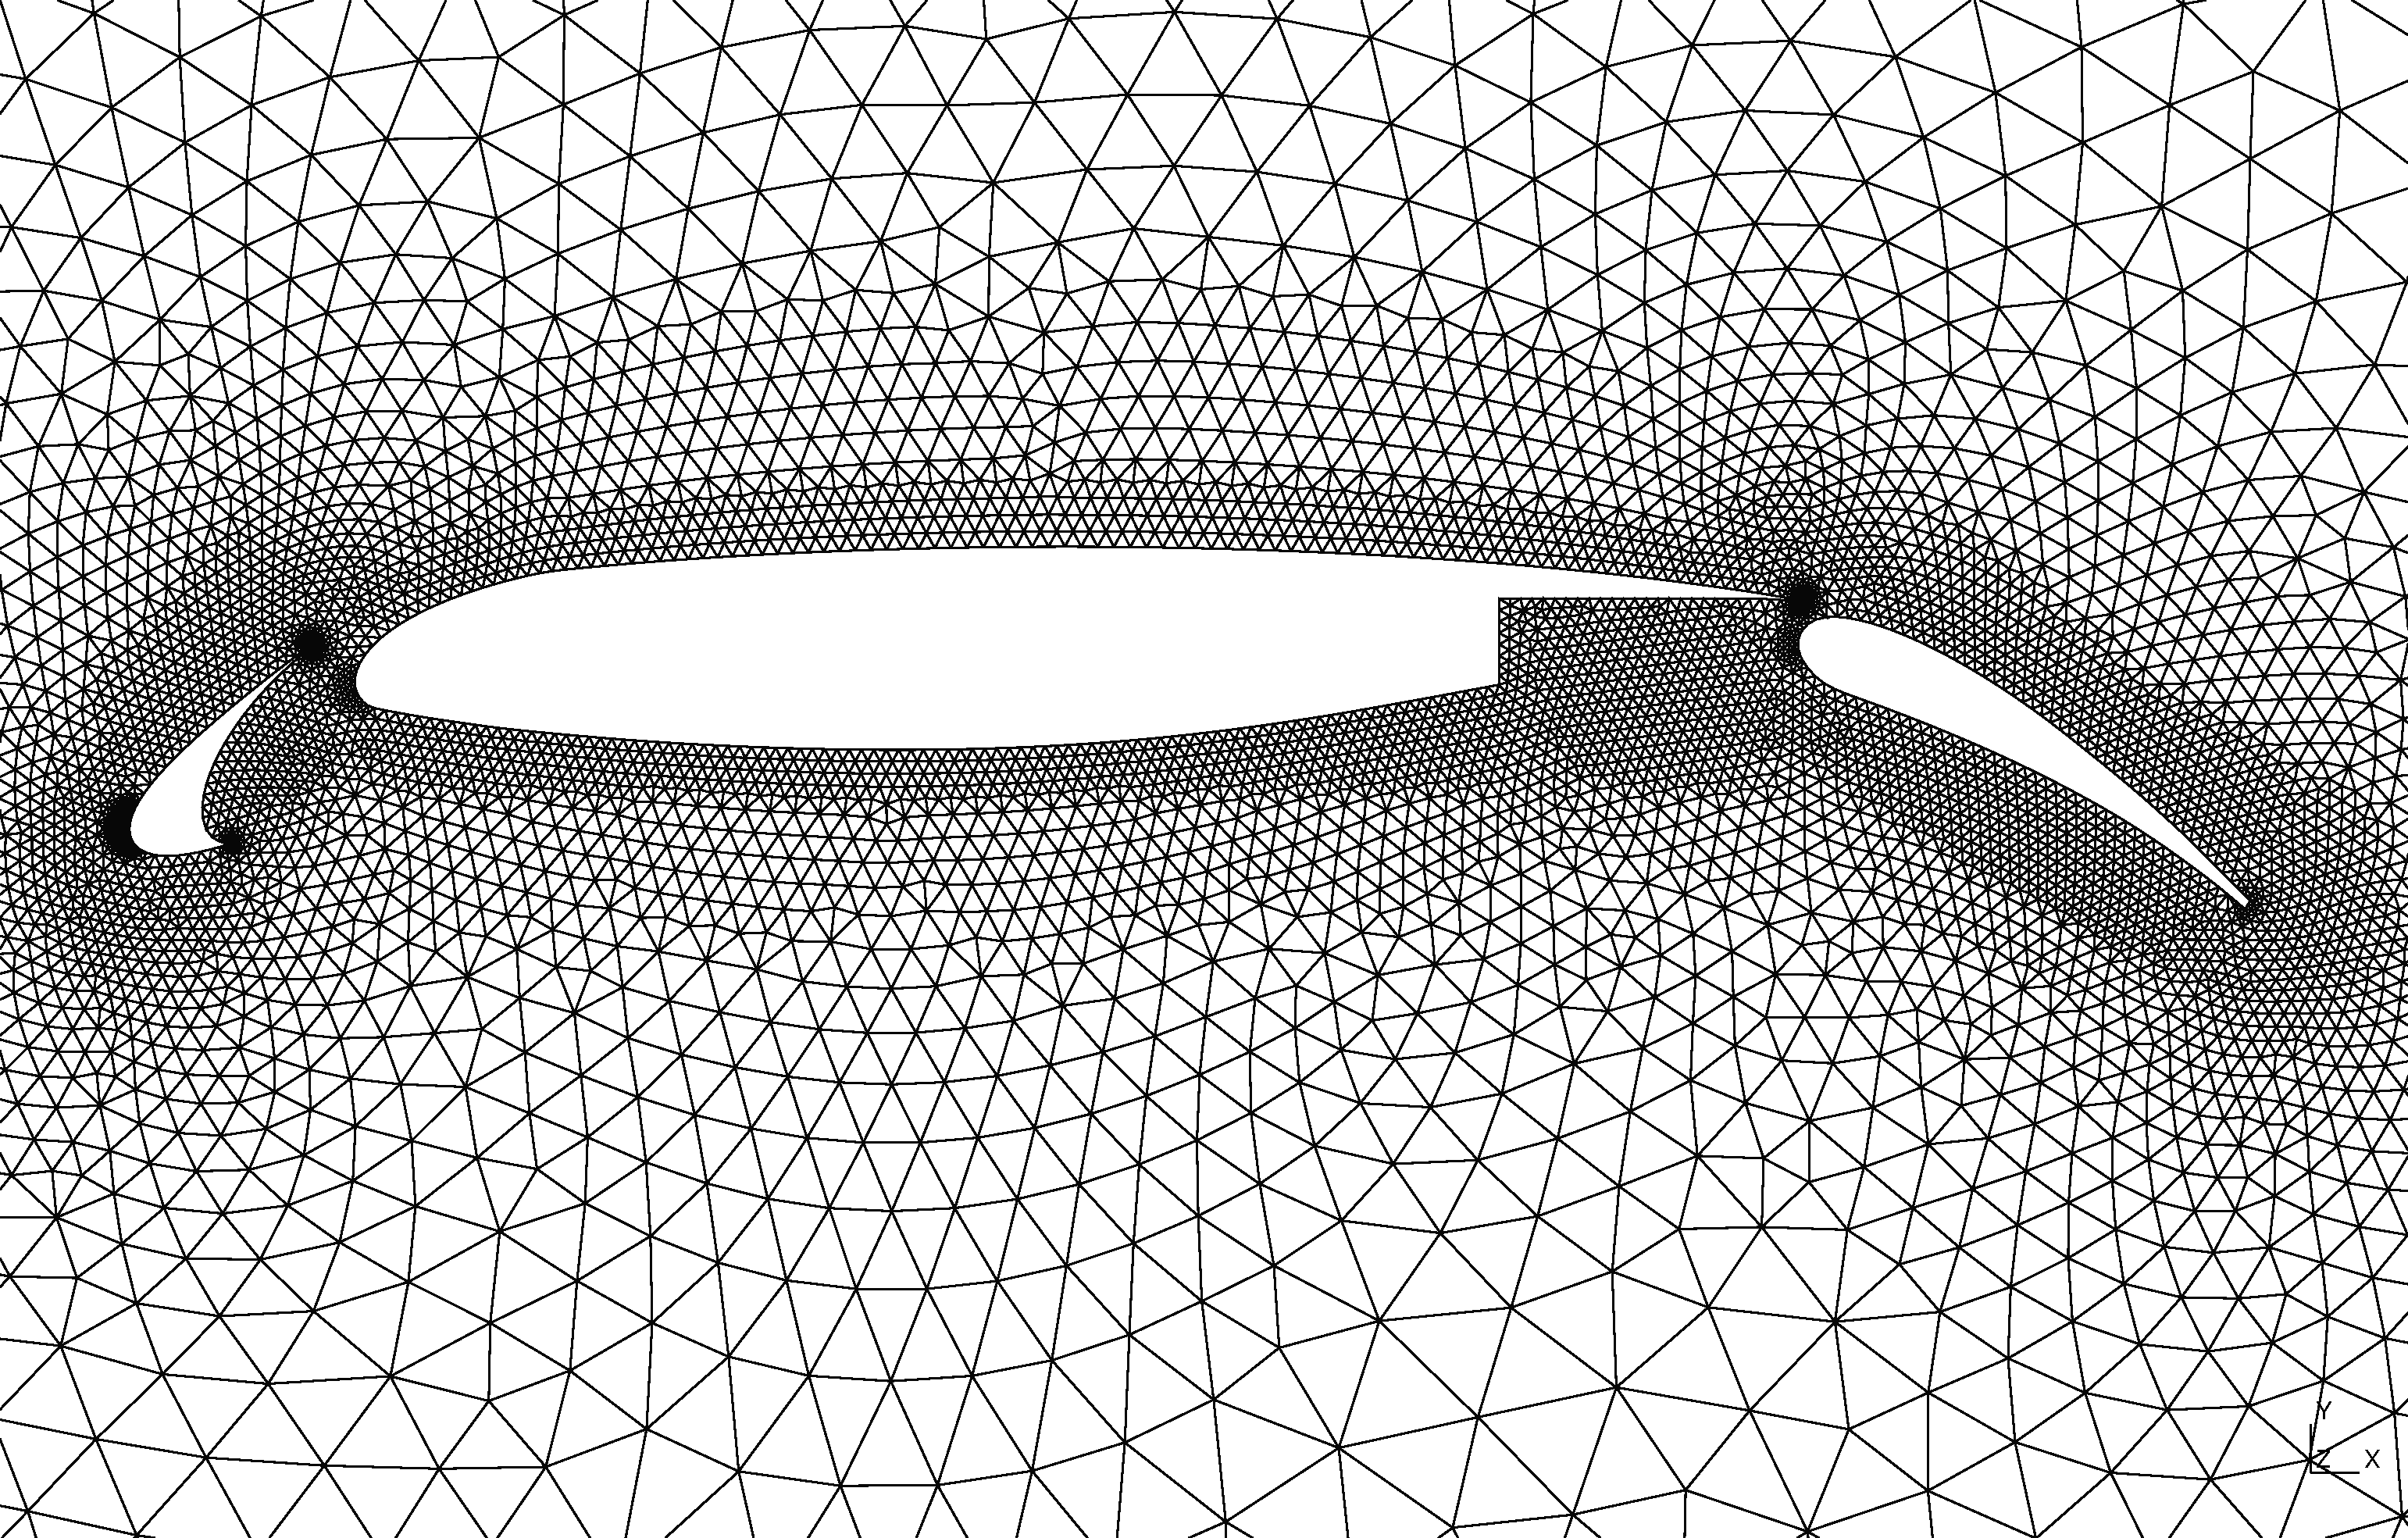
\includegraphics[scale=0.16]{3comp-inviscid}
	\caption{Original mesh for inviscid flow around 3-component airfoil}
	\label{fig:wing-inviscid}
\end{figure}
\end{frame}

\begin{frame}{Torsion springs}
	\begin{figure}[!h]
		\centering
		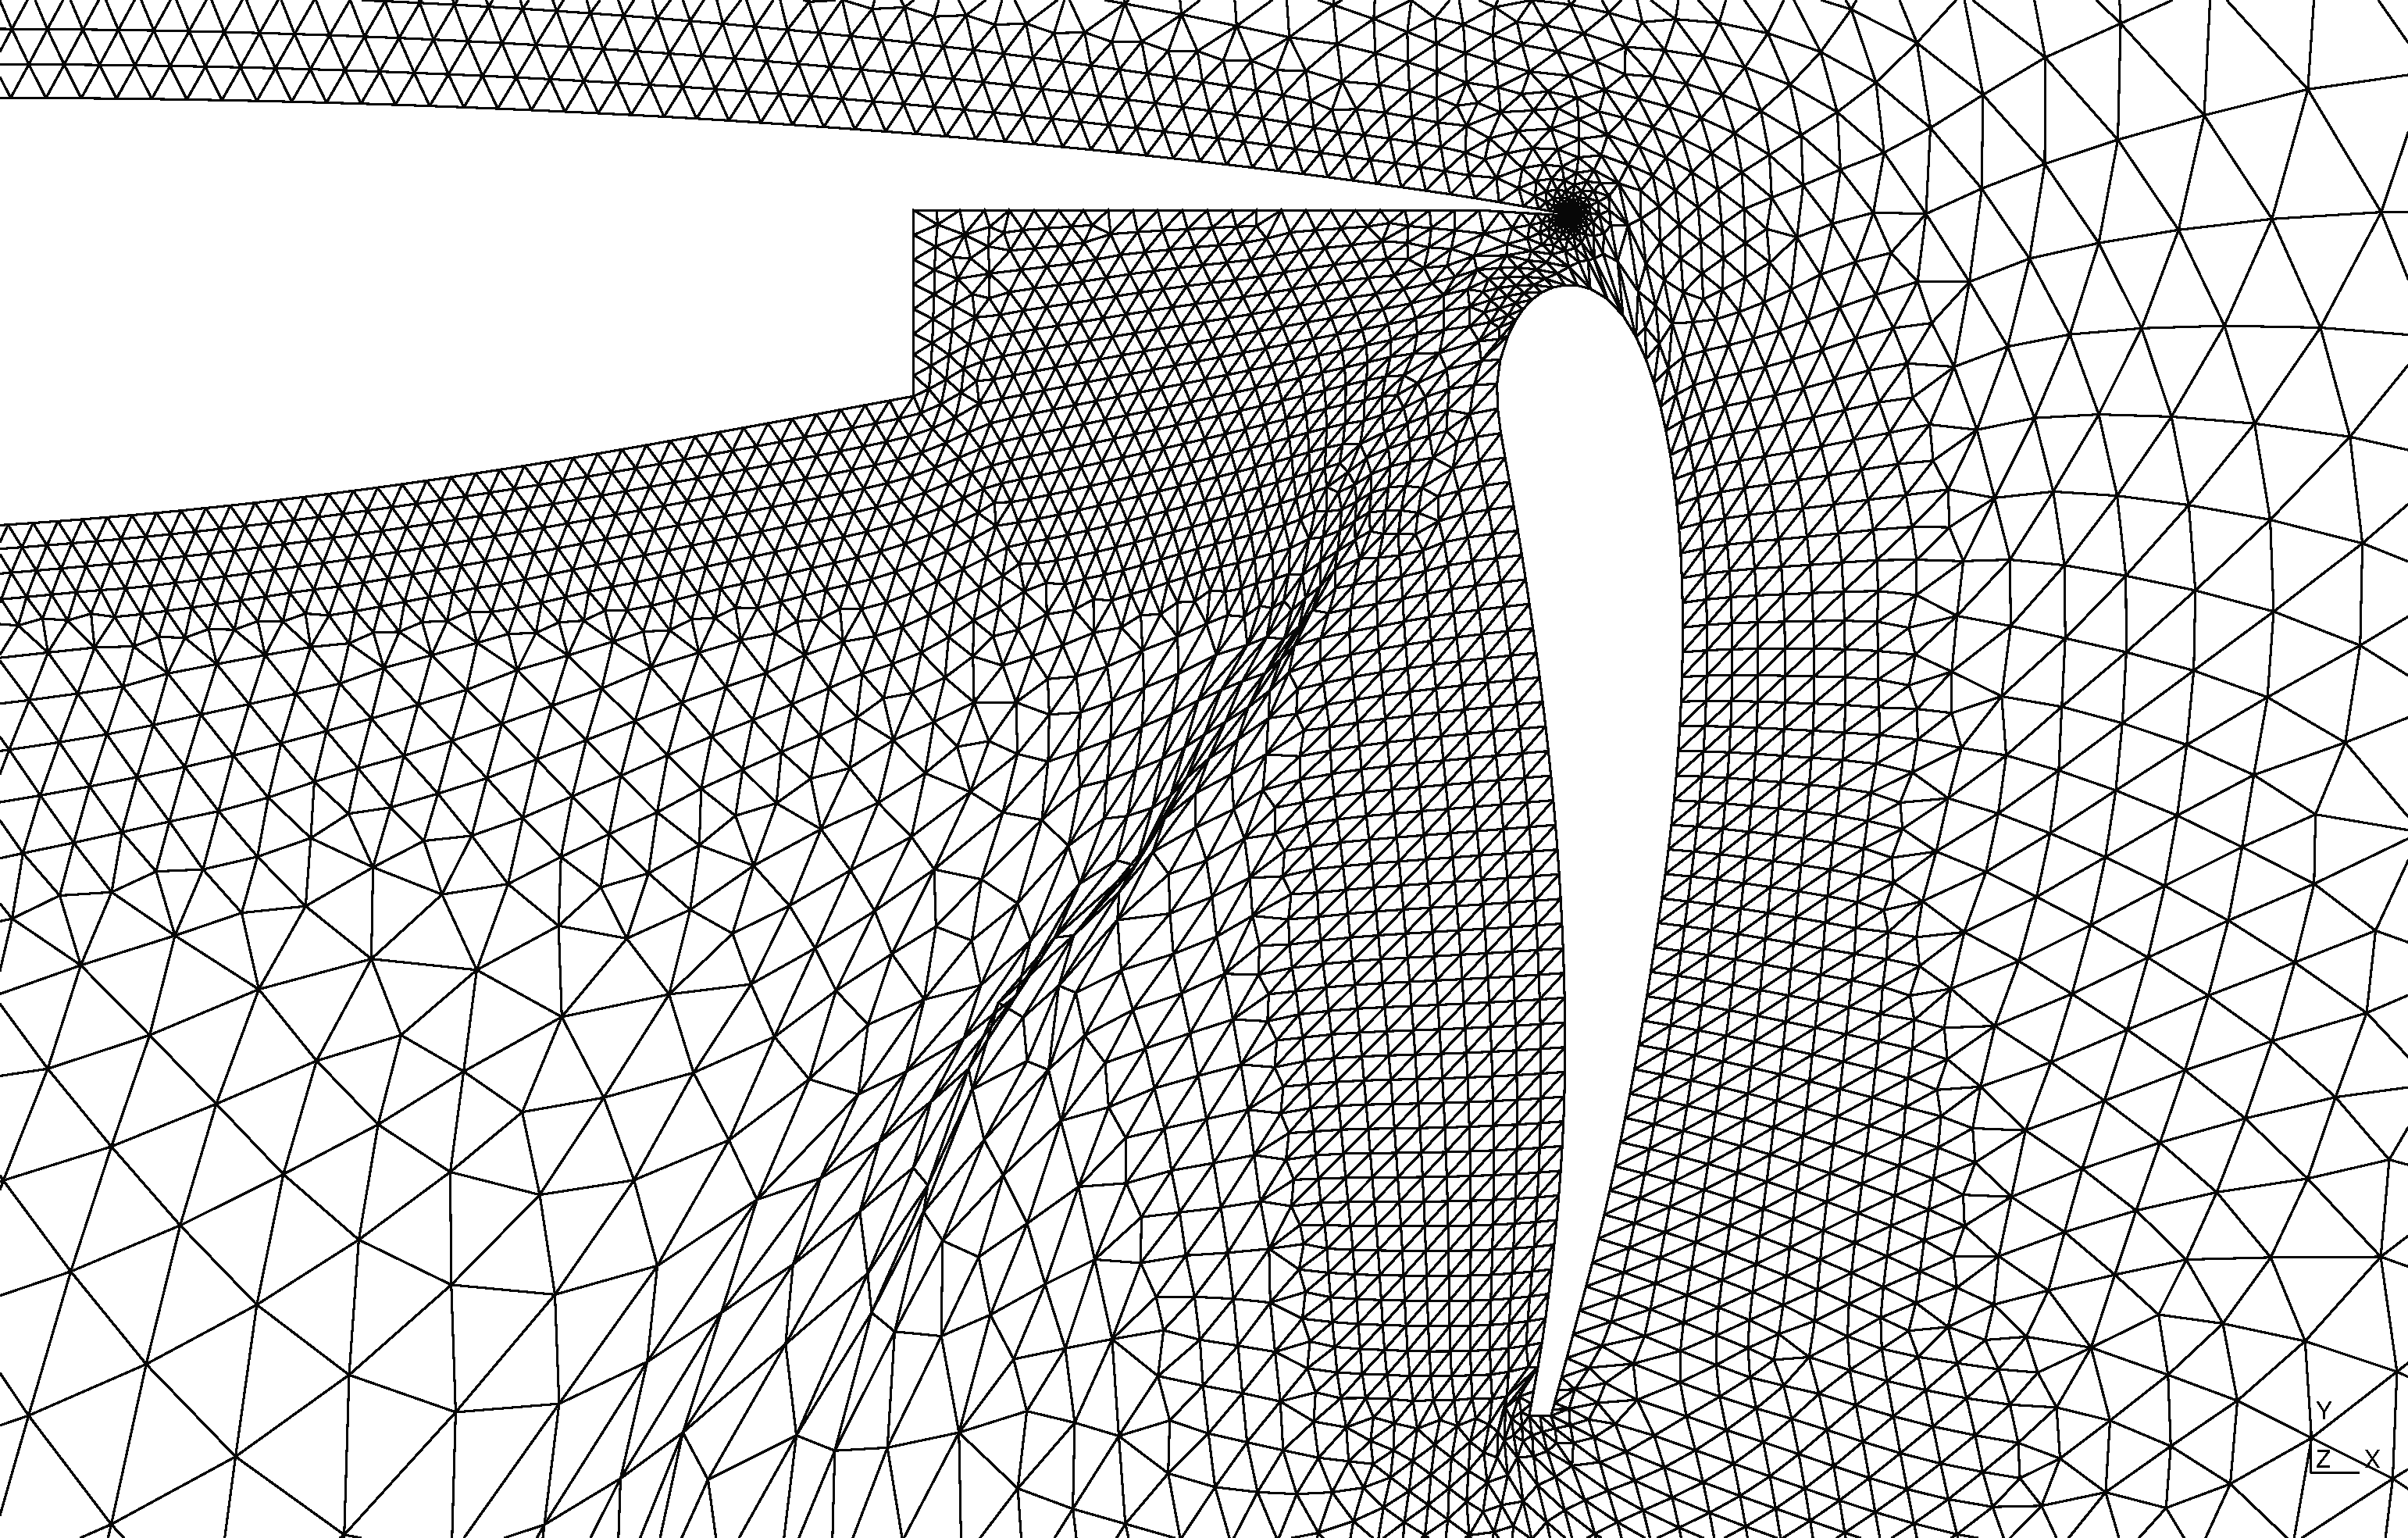
\includegraphics[scale=0.17]{wing60-farhat}
		\caption{Inviscid 3-component airfoil mesh with 60$^\circ$ rotation of flap by torsion spring method}
		\label{fig:wing-inviscid-farhat}
	\end{figure}
	Cells near the trailing edge of the middle wing do not suffer much degradation, but cells somewhat farther away become invalid
\end{frame}

\begin{frame}{Linear elasticity}
	\begin{figure}[!h]
		\centering
		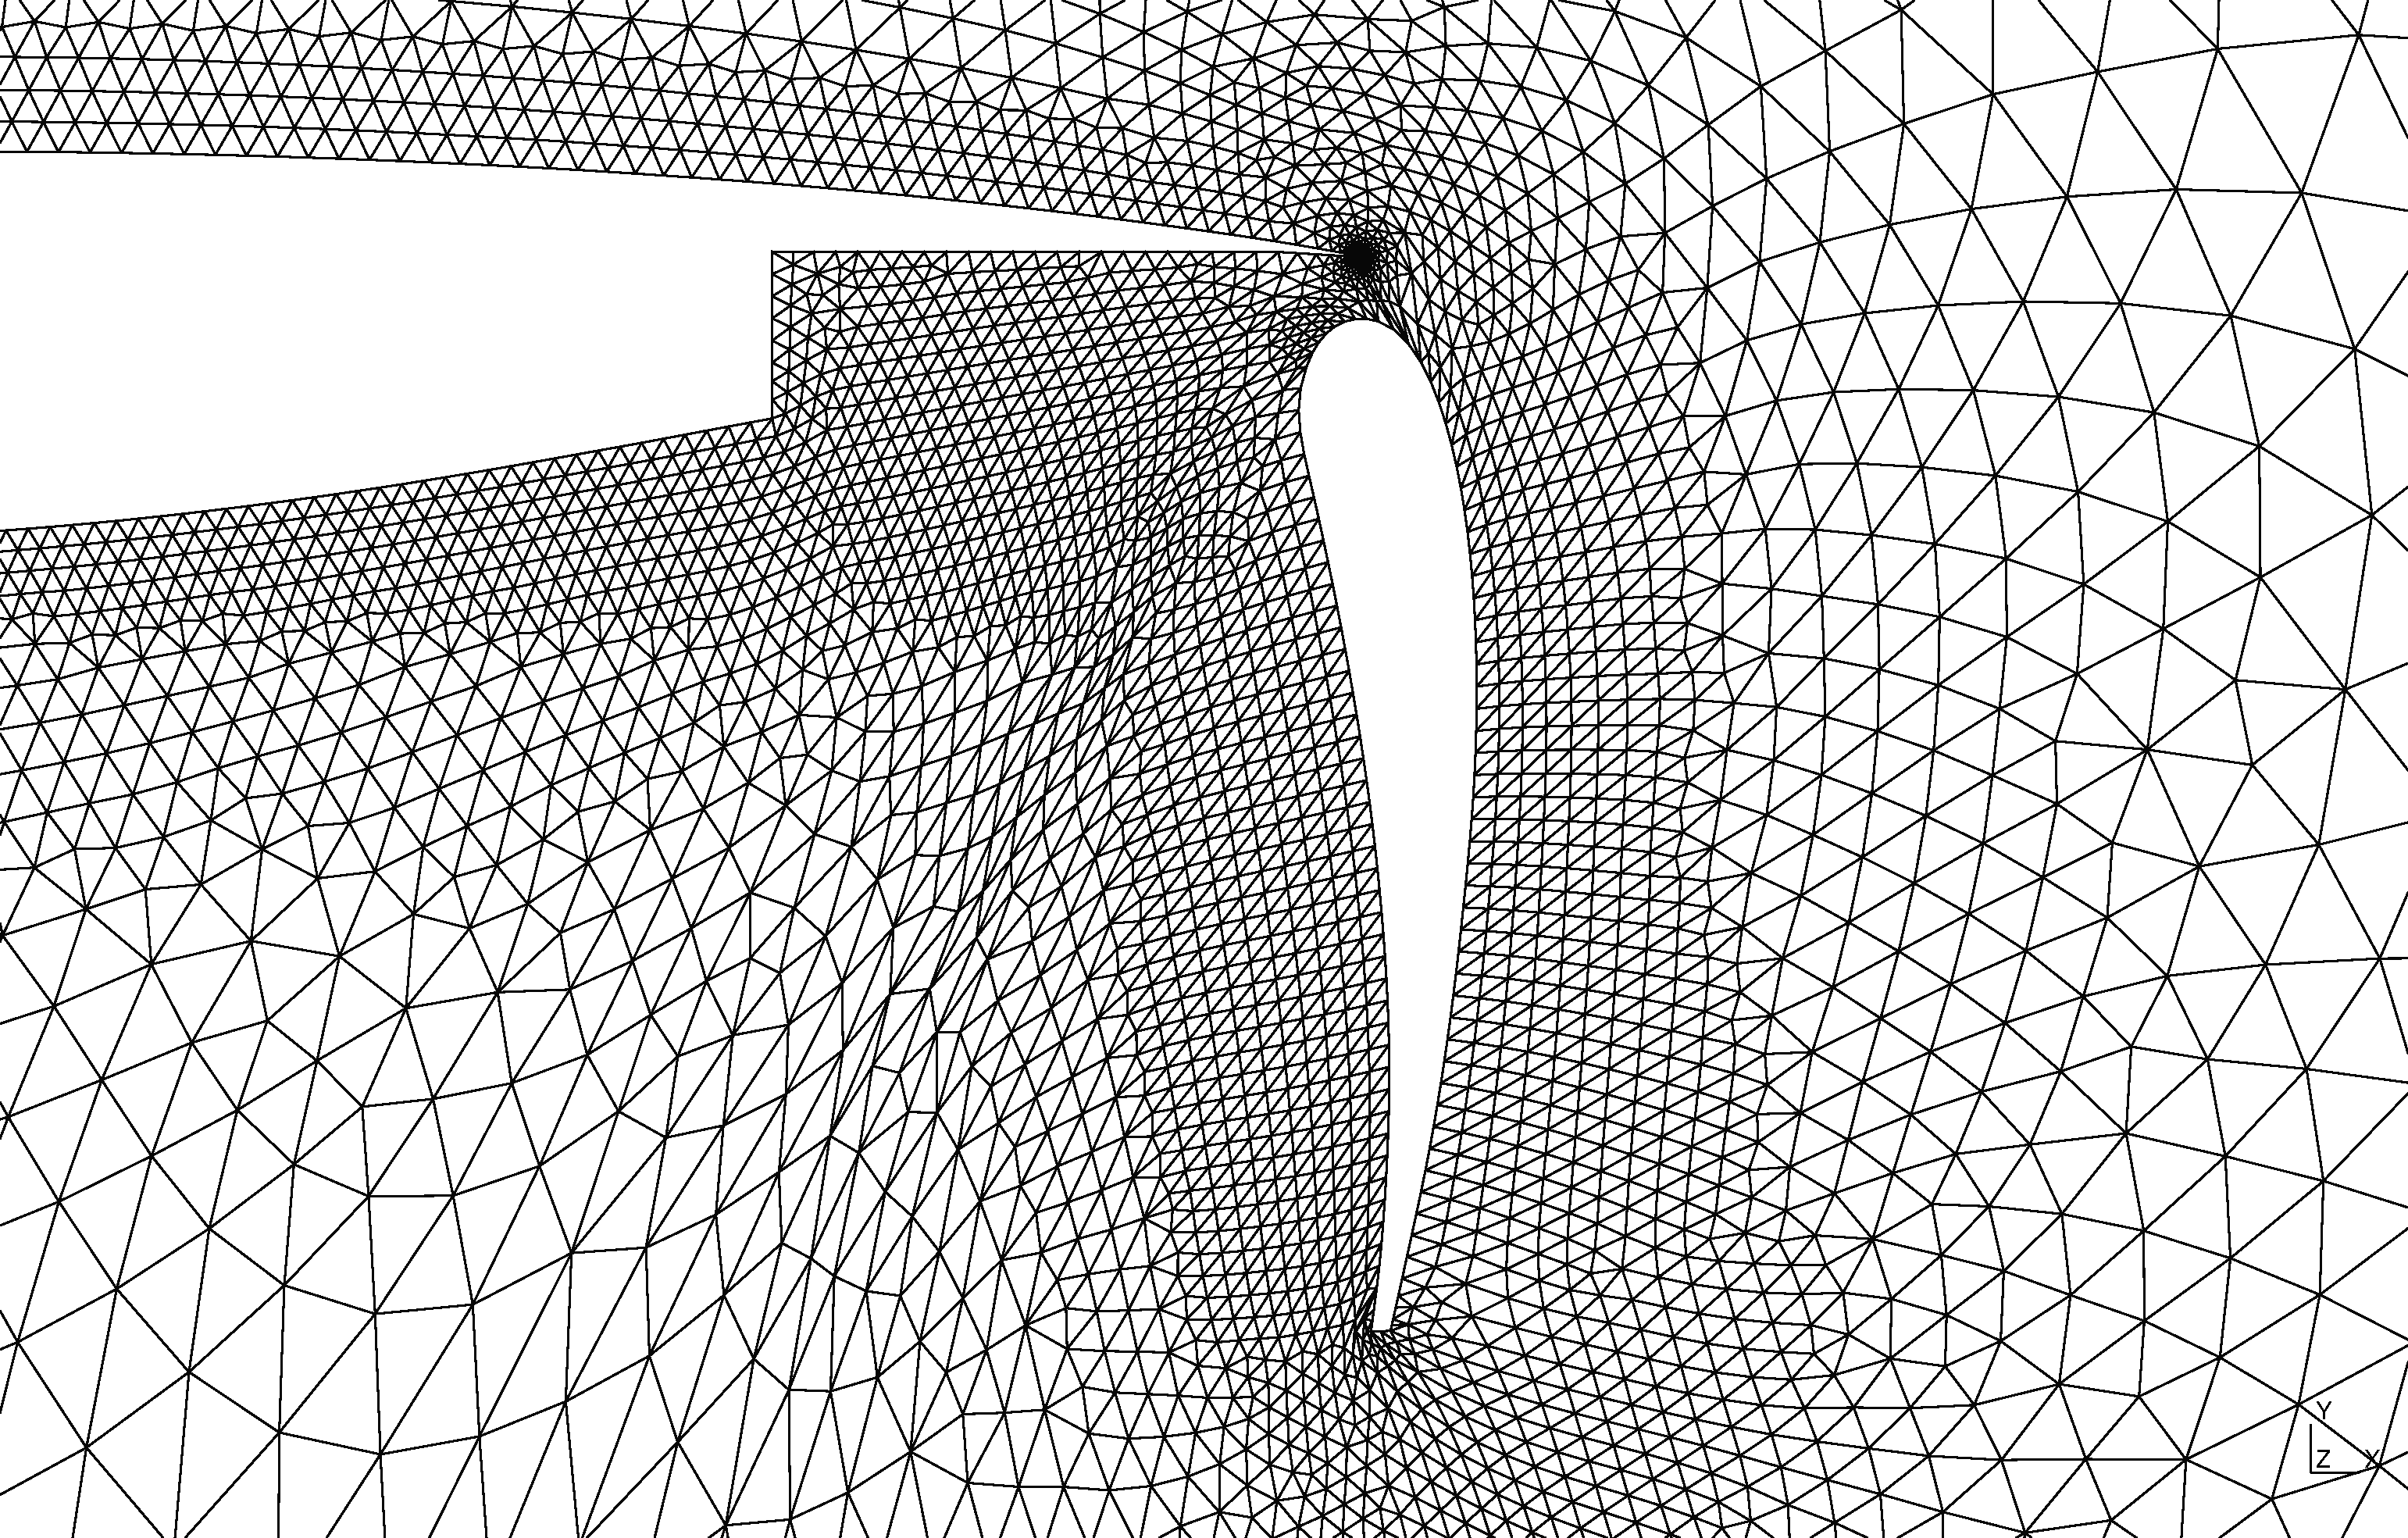
\includegraphics[scale=0.17]{wing60-linelastp1}
		\caption{Inviscid 3-component airfoil mesh with 60$^\circ$ rotation of flap by linear elasticity method}
		\label{fig:wing-inviscid-linelastp1}
	\end{figure}
\end{frame}
\begin{frame}{Linear elasticity}
	\begin{figure}[!h]
		\centering
		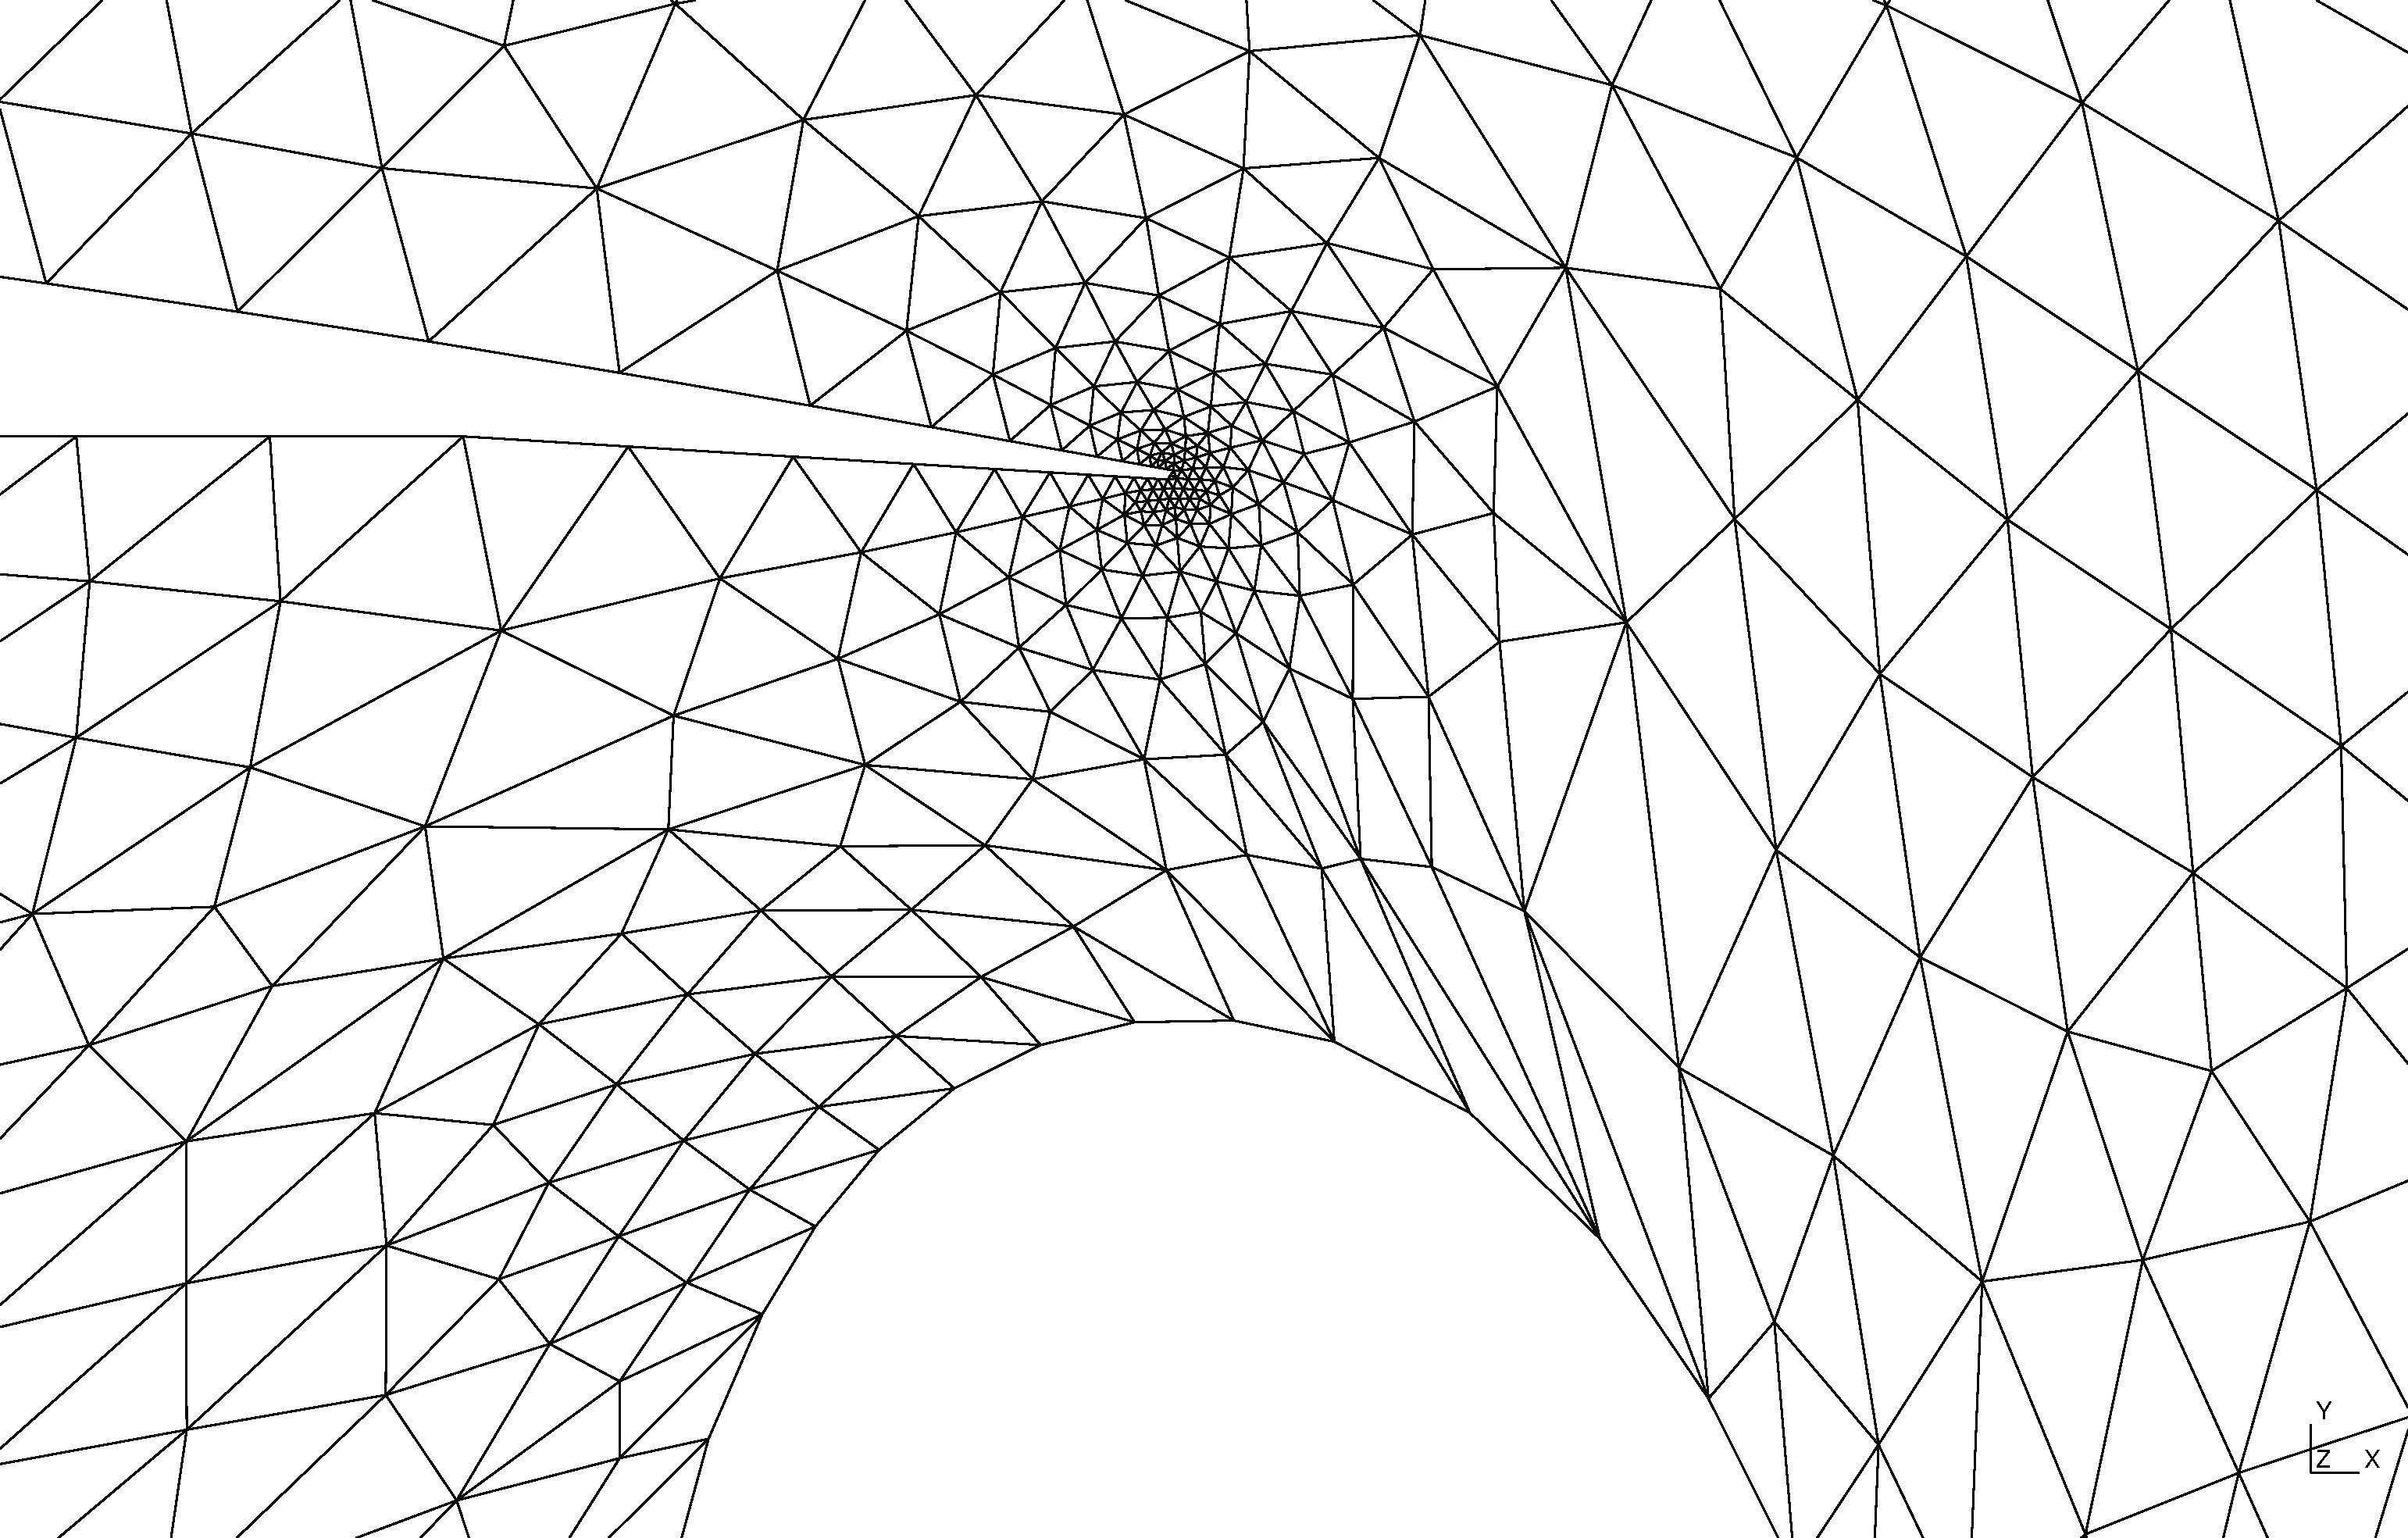
\includegraphics[scale=0.17]{wing60-linelastp1_zoomed}
		\caption{Inviscid 3-component airfoil mesh with 60$^\circ$ rotation of flap by linear elasticity method; zoomed to where the flap meets the wing}
		\label{fig:wing-inviscid-linelastp1-zoomed}
	\end{figure}
\end{frame}
\begin{frame}{Linear elasticity}
	\begin{figure}[!h]
		\centering
		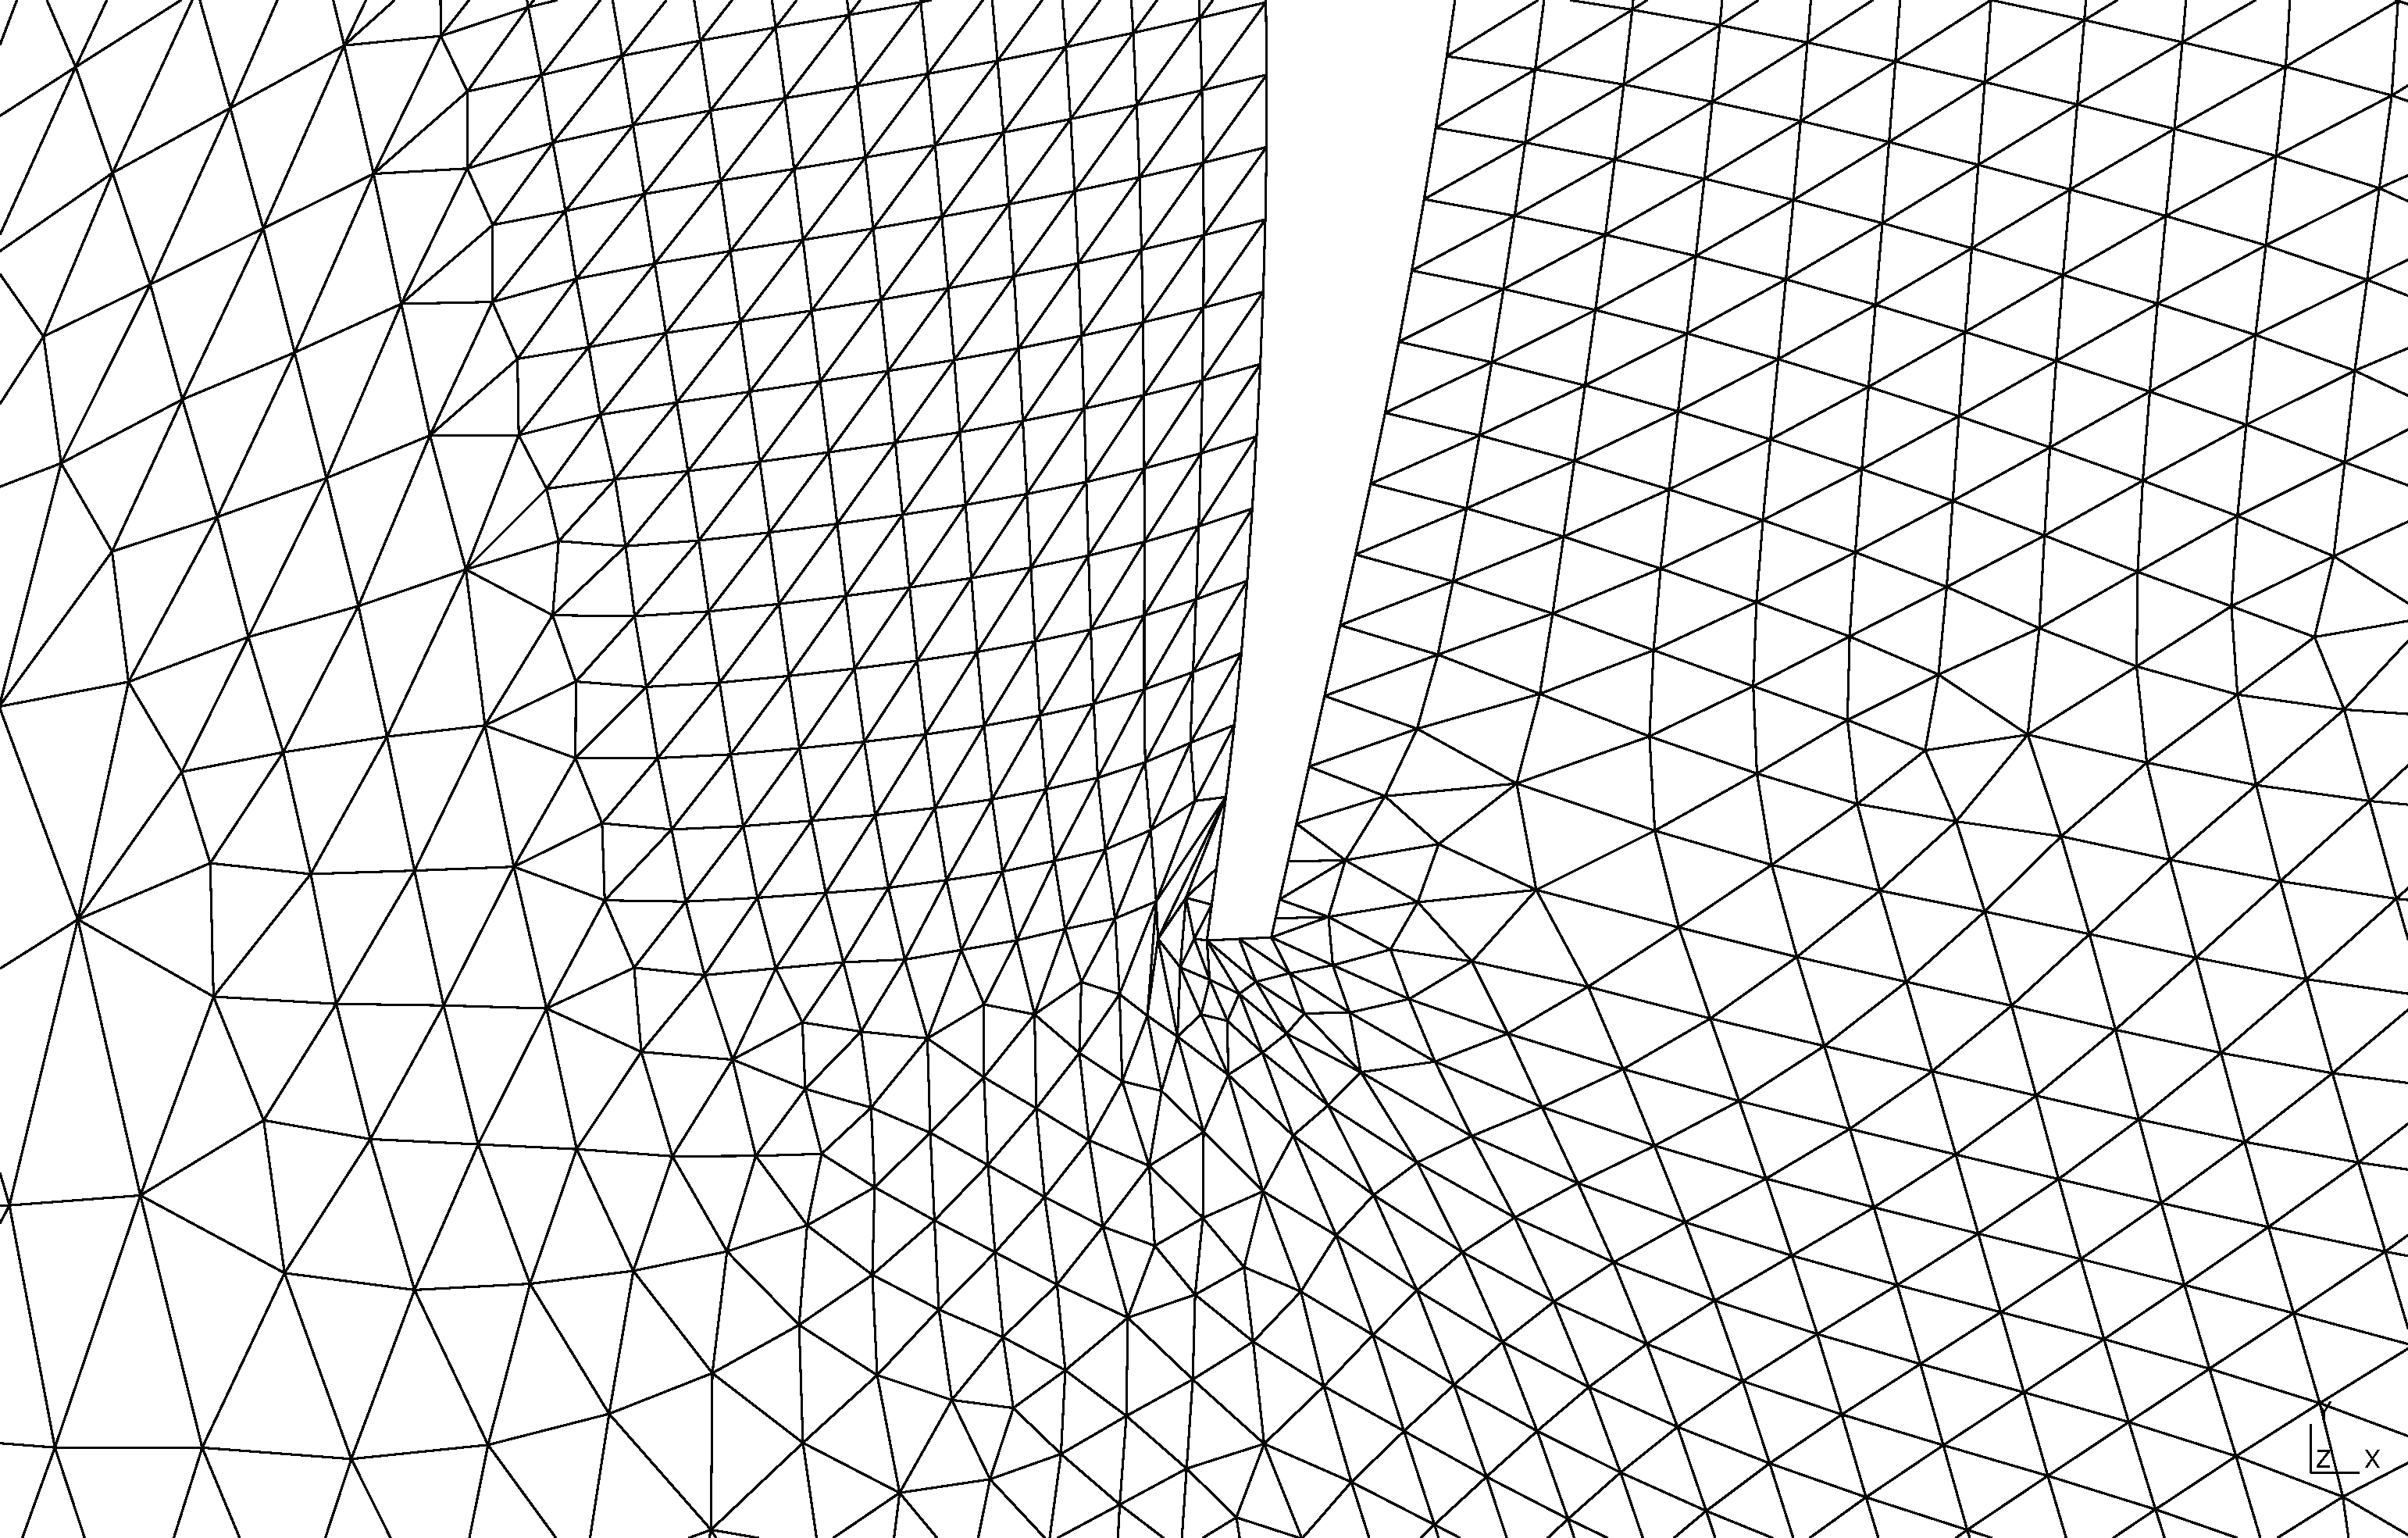
\includegraphics[scale=0.17]{wing60-linelastp1_zoomed2}
		\caption{Inviscid 3-component airfoil mesh with 60$^\circ$ rotation of flap by linear elasticity method, zoomed to the trailing edge of the flap}
		\label{fig:wing-inviscid-linelastp1-zoomed2}
	\end{figure}
\end{frame}
\begin{frame}{DGM}
	\begin{figure}[!h]
		\centering
		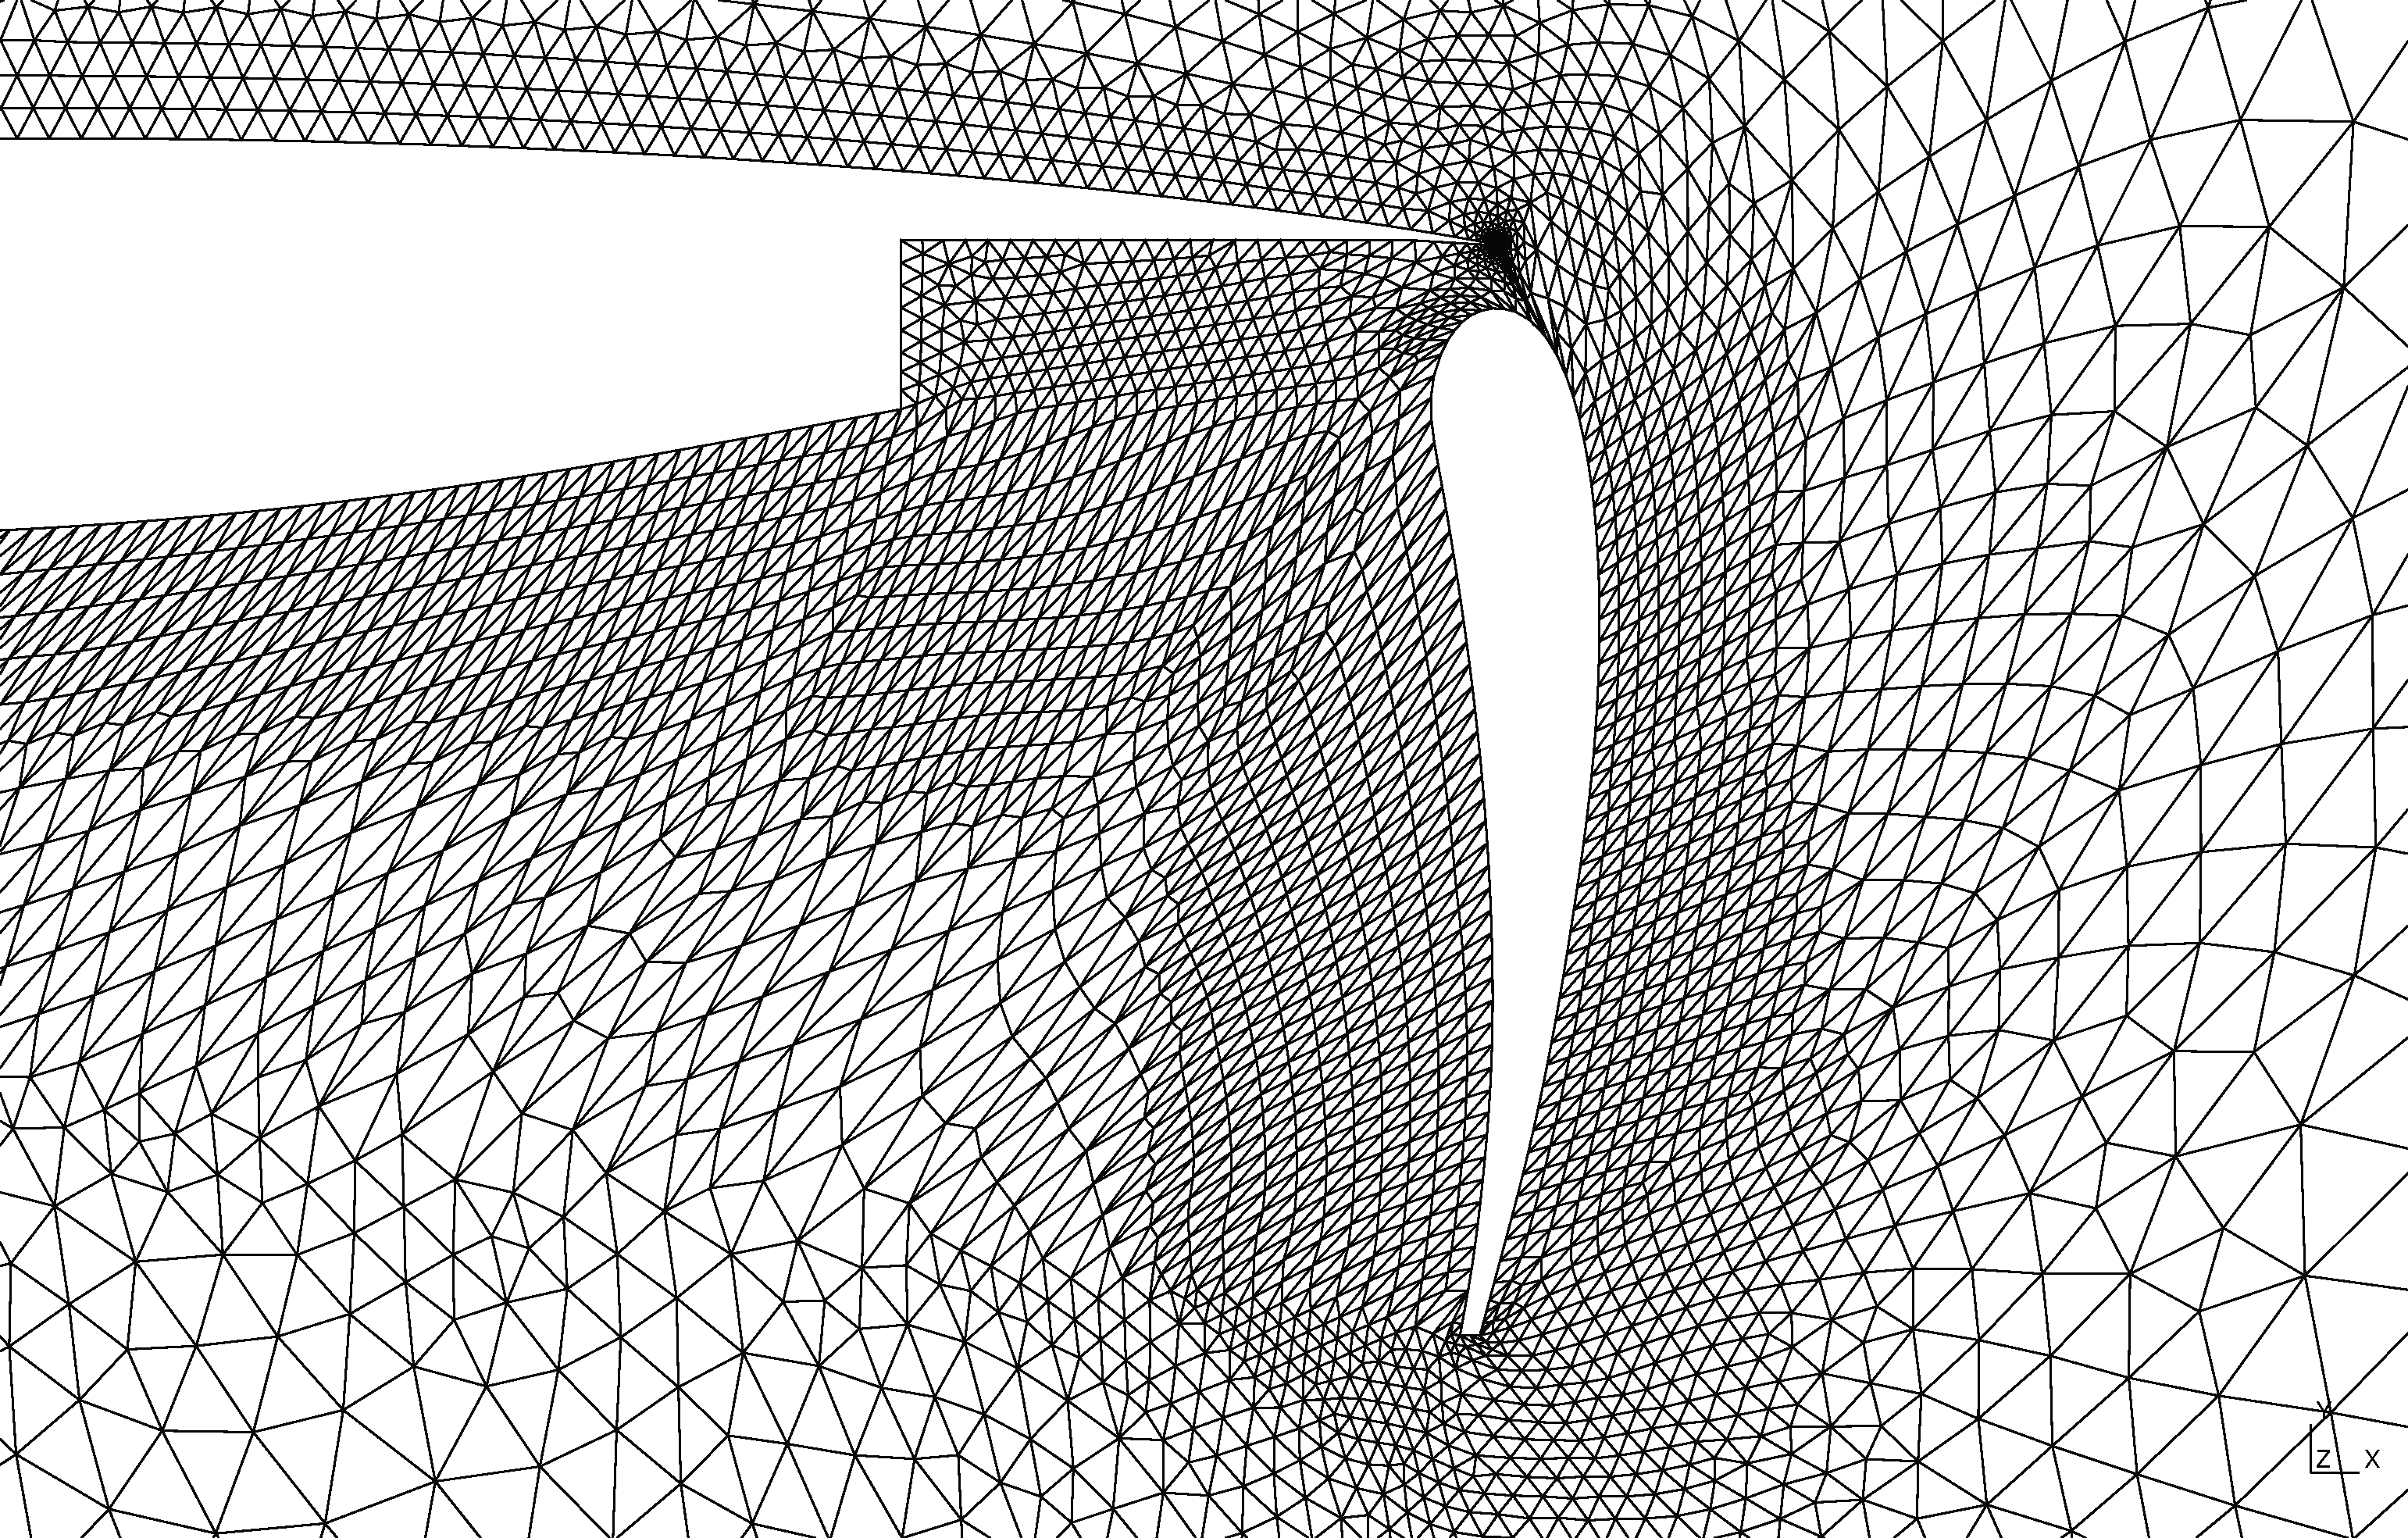
\includegraphics[scale=0.17]{wing60-dg-ms}
		\caption{Inviscid 3-component airfoil mesh with 60$^\circ$ rotation of flap by DGM method}
		\label{fig:wing-inviscid-dg-ms}
	\end{figure}
\end{frame}
\begin{frame}{DGM}
	\begin{figure}[!h]
		\centering
		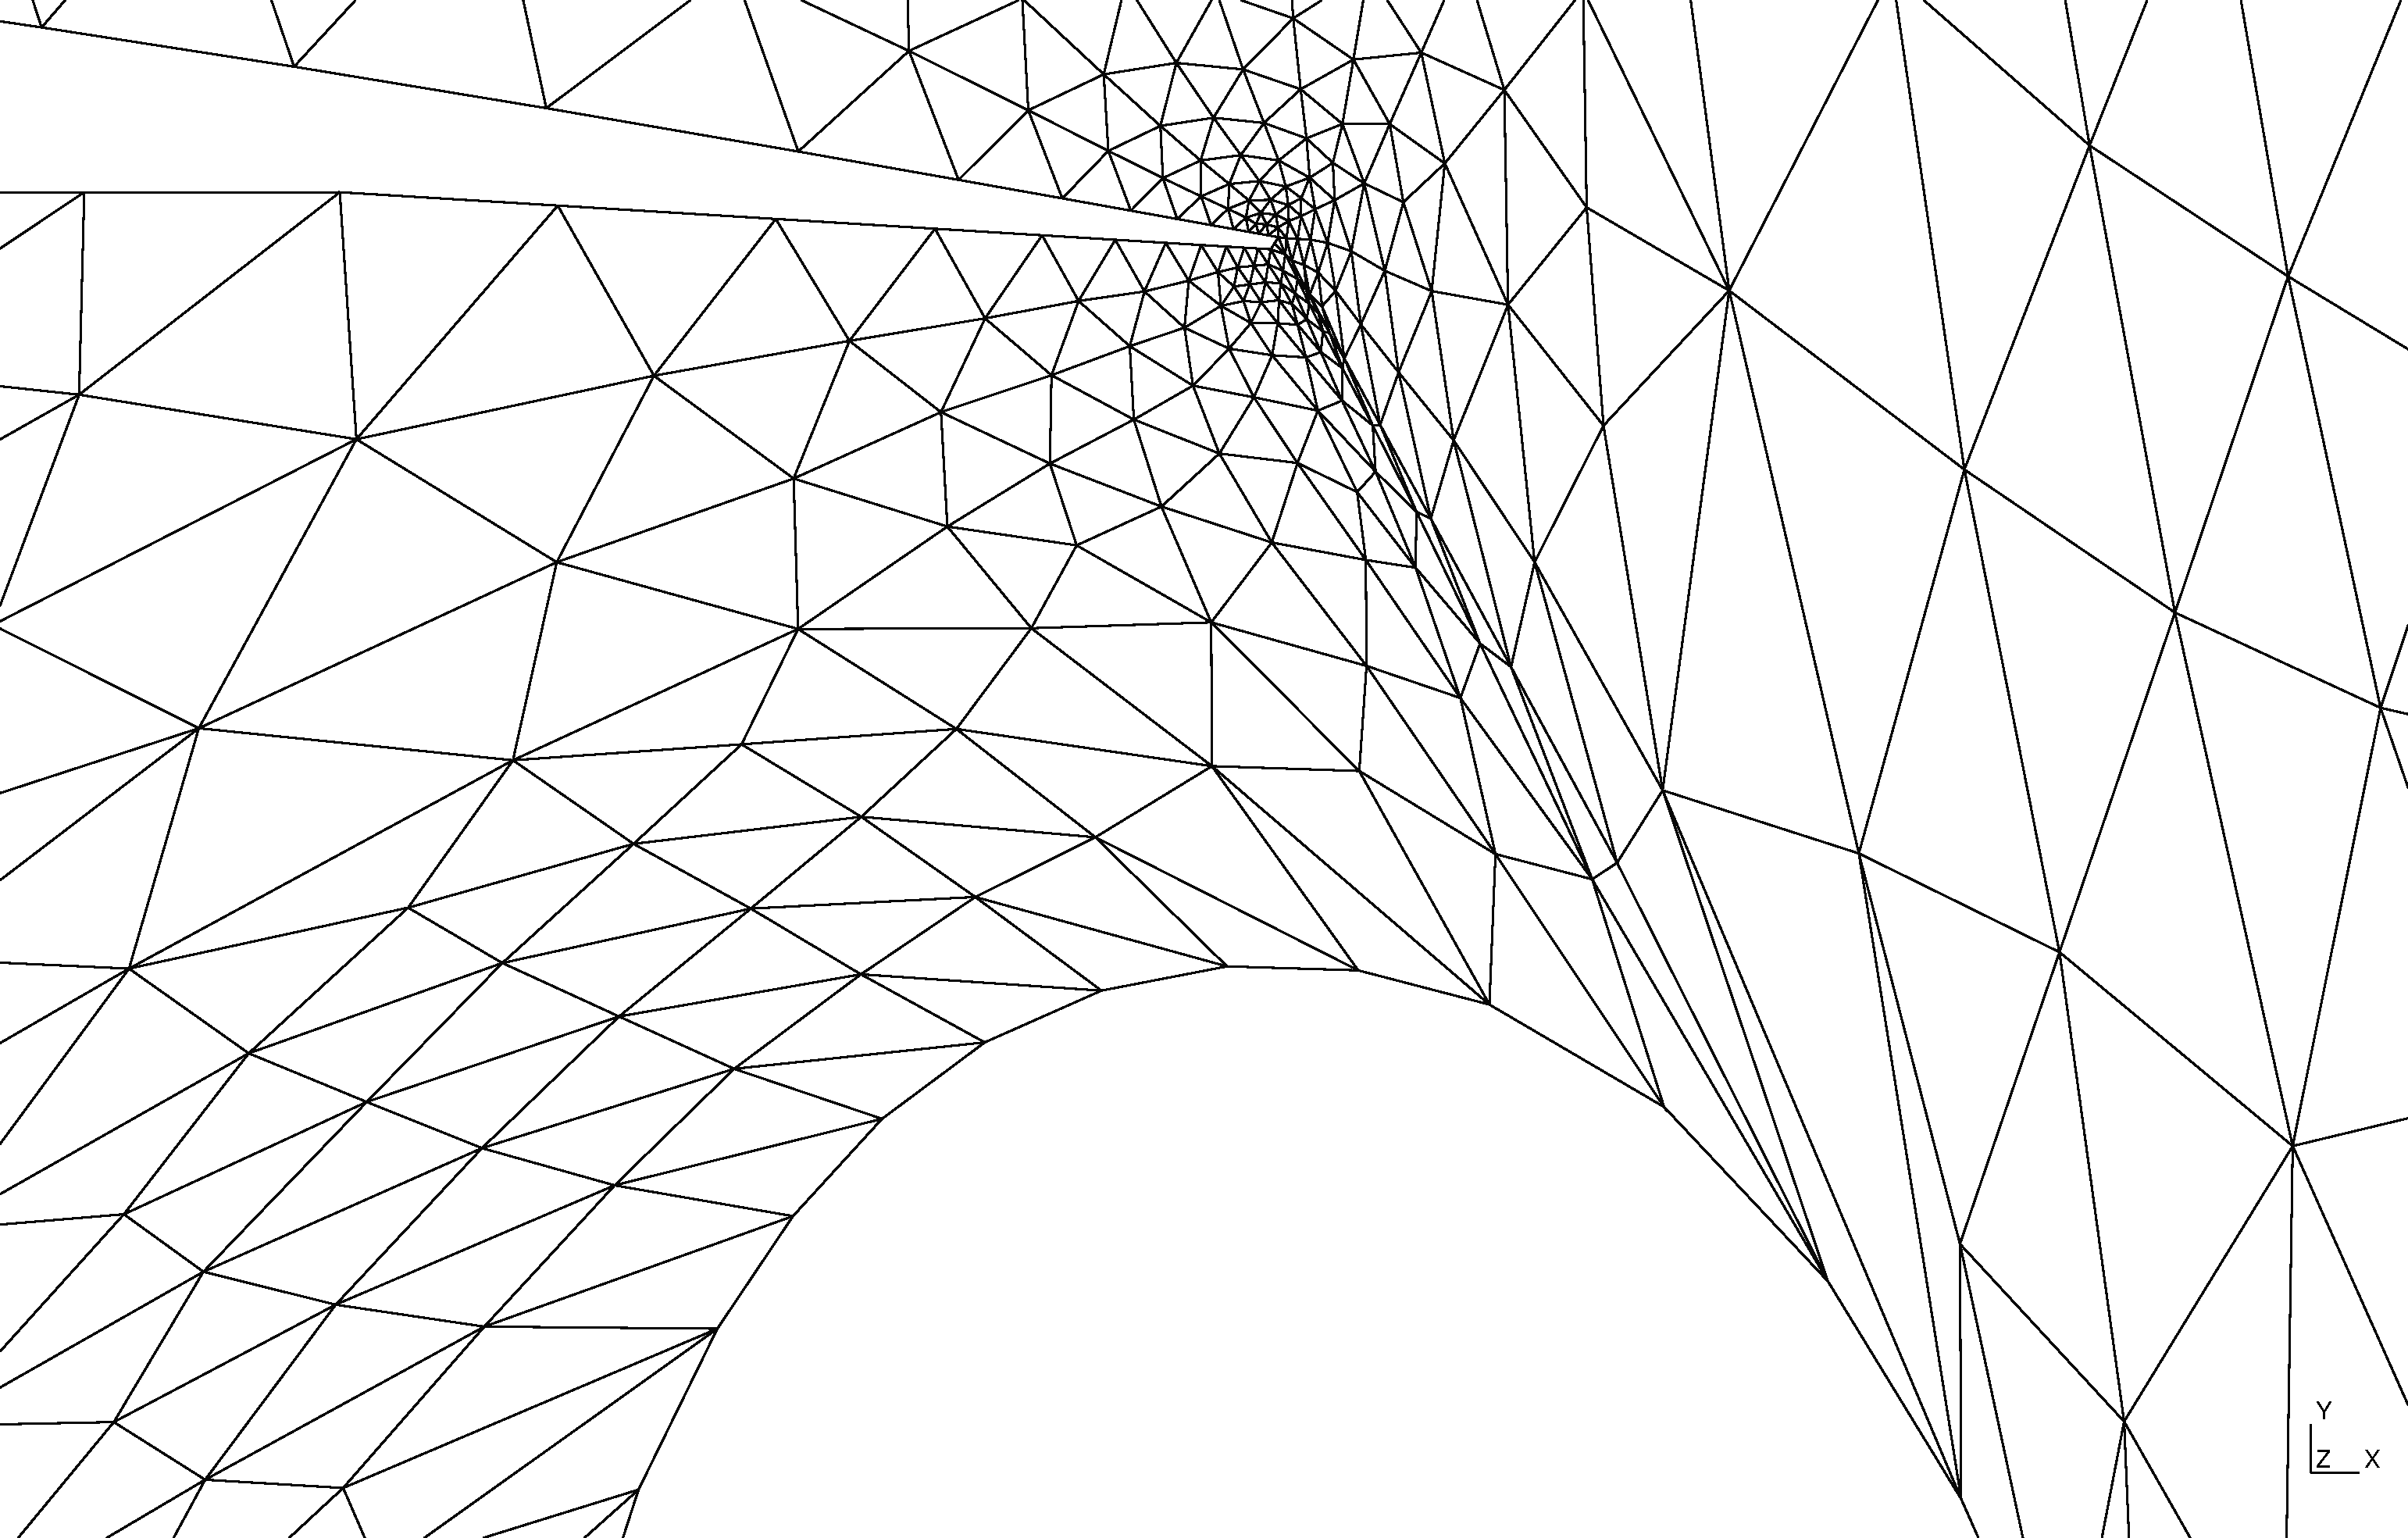
\includegraphics[scale=0.17]{wing60-dg-ms_zoomed}
		\caption{Inviscid 3-component airfoil mesh with 60$^\circ$ rotation of flap by DGM method; zoomed to where the flap meets the wing}
		\label{fig:wing-inviscid-dg-ms-zoomed}
	\end{figure}
\end{frame}

\begin{frame}{RBF}
\begin{figure}
	\centering
	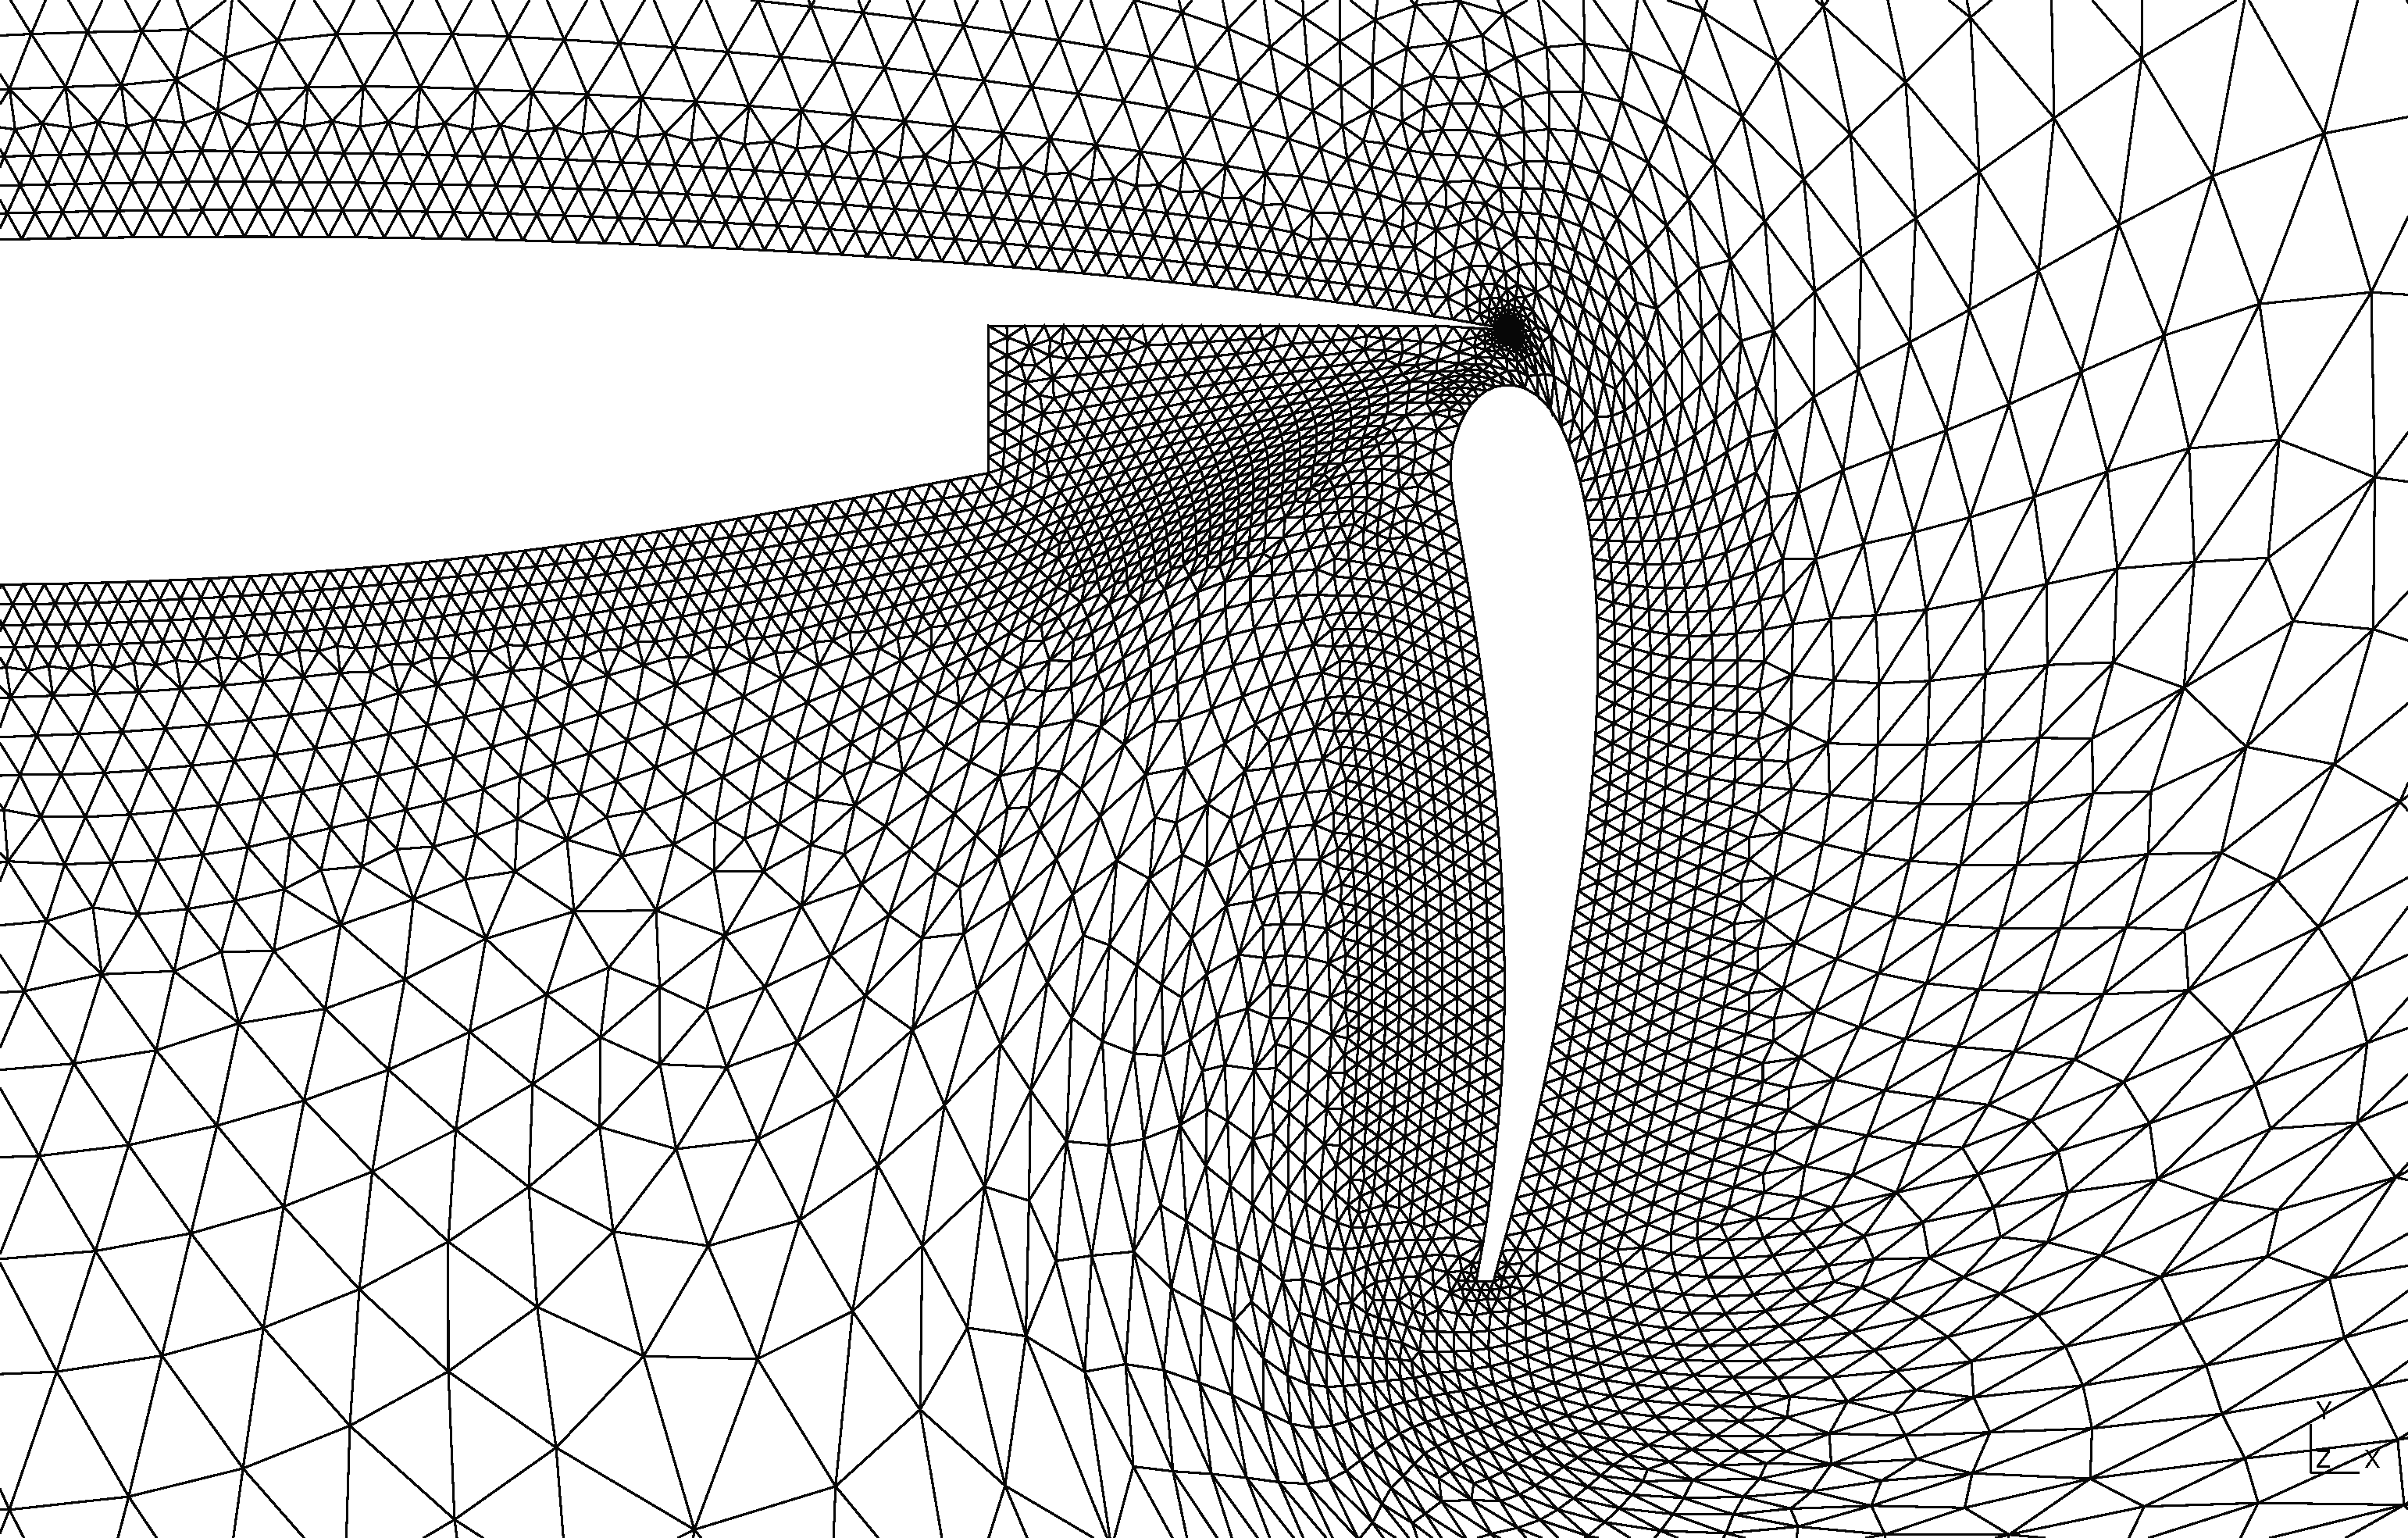
\includegraphics[scale=0.17]{wing60-rbf-sr15-s3}
	\caption{Inviscid 3-component airfoil mesh with 60$^\circ$ rotation of flap by RBF method}
	\label{fig:wing-inviscid-rbf}
\end{figure}
\end{frame}
\begin{frame}{RBF}
\begin{figure}
	\centering
	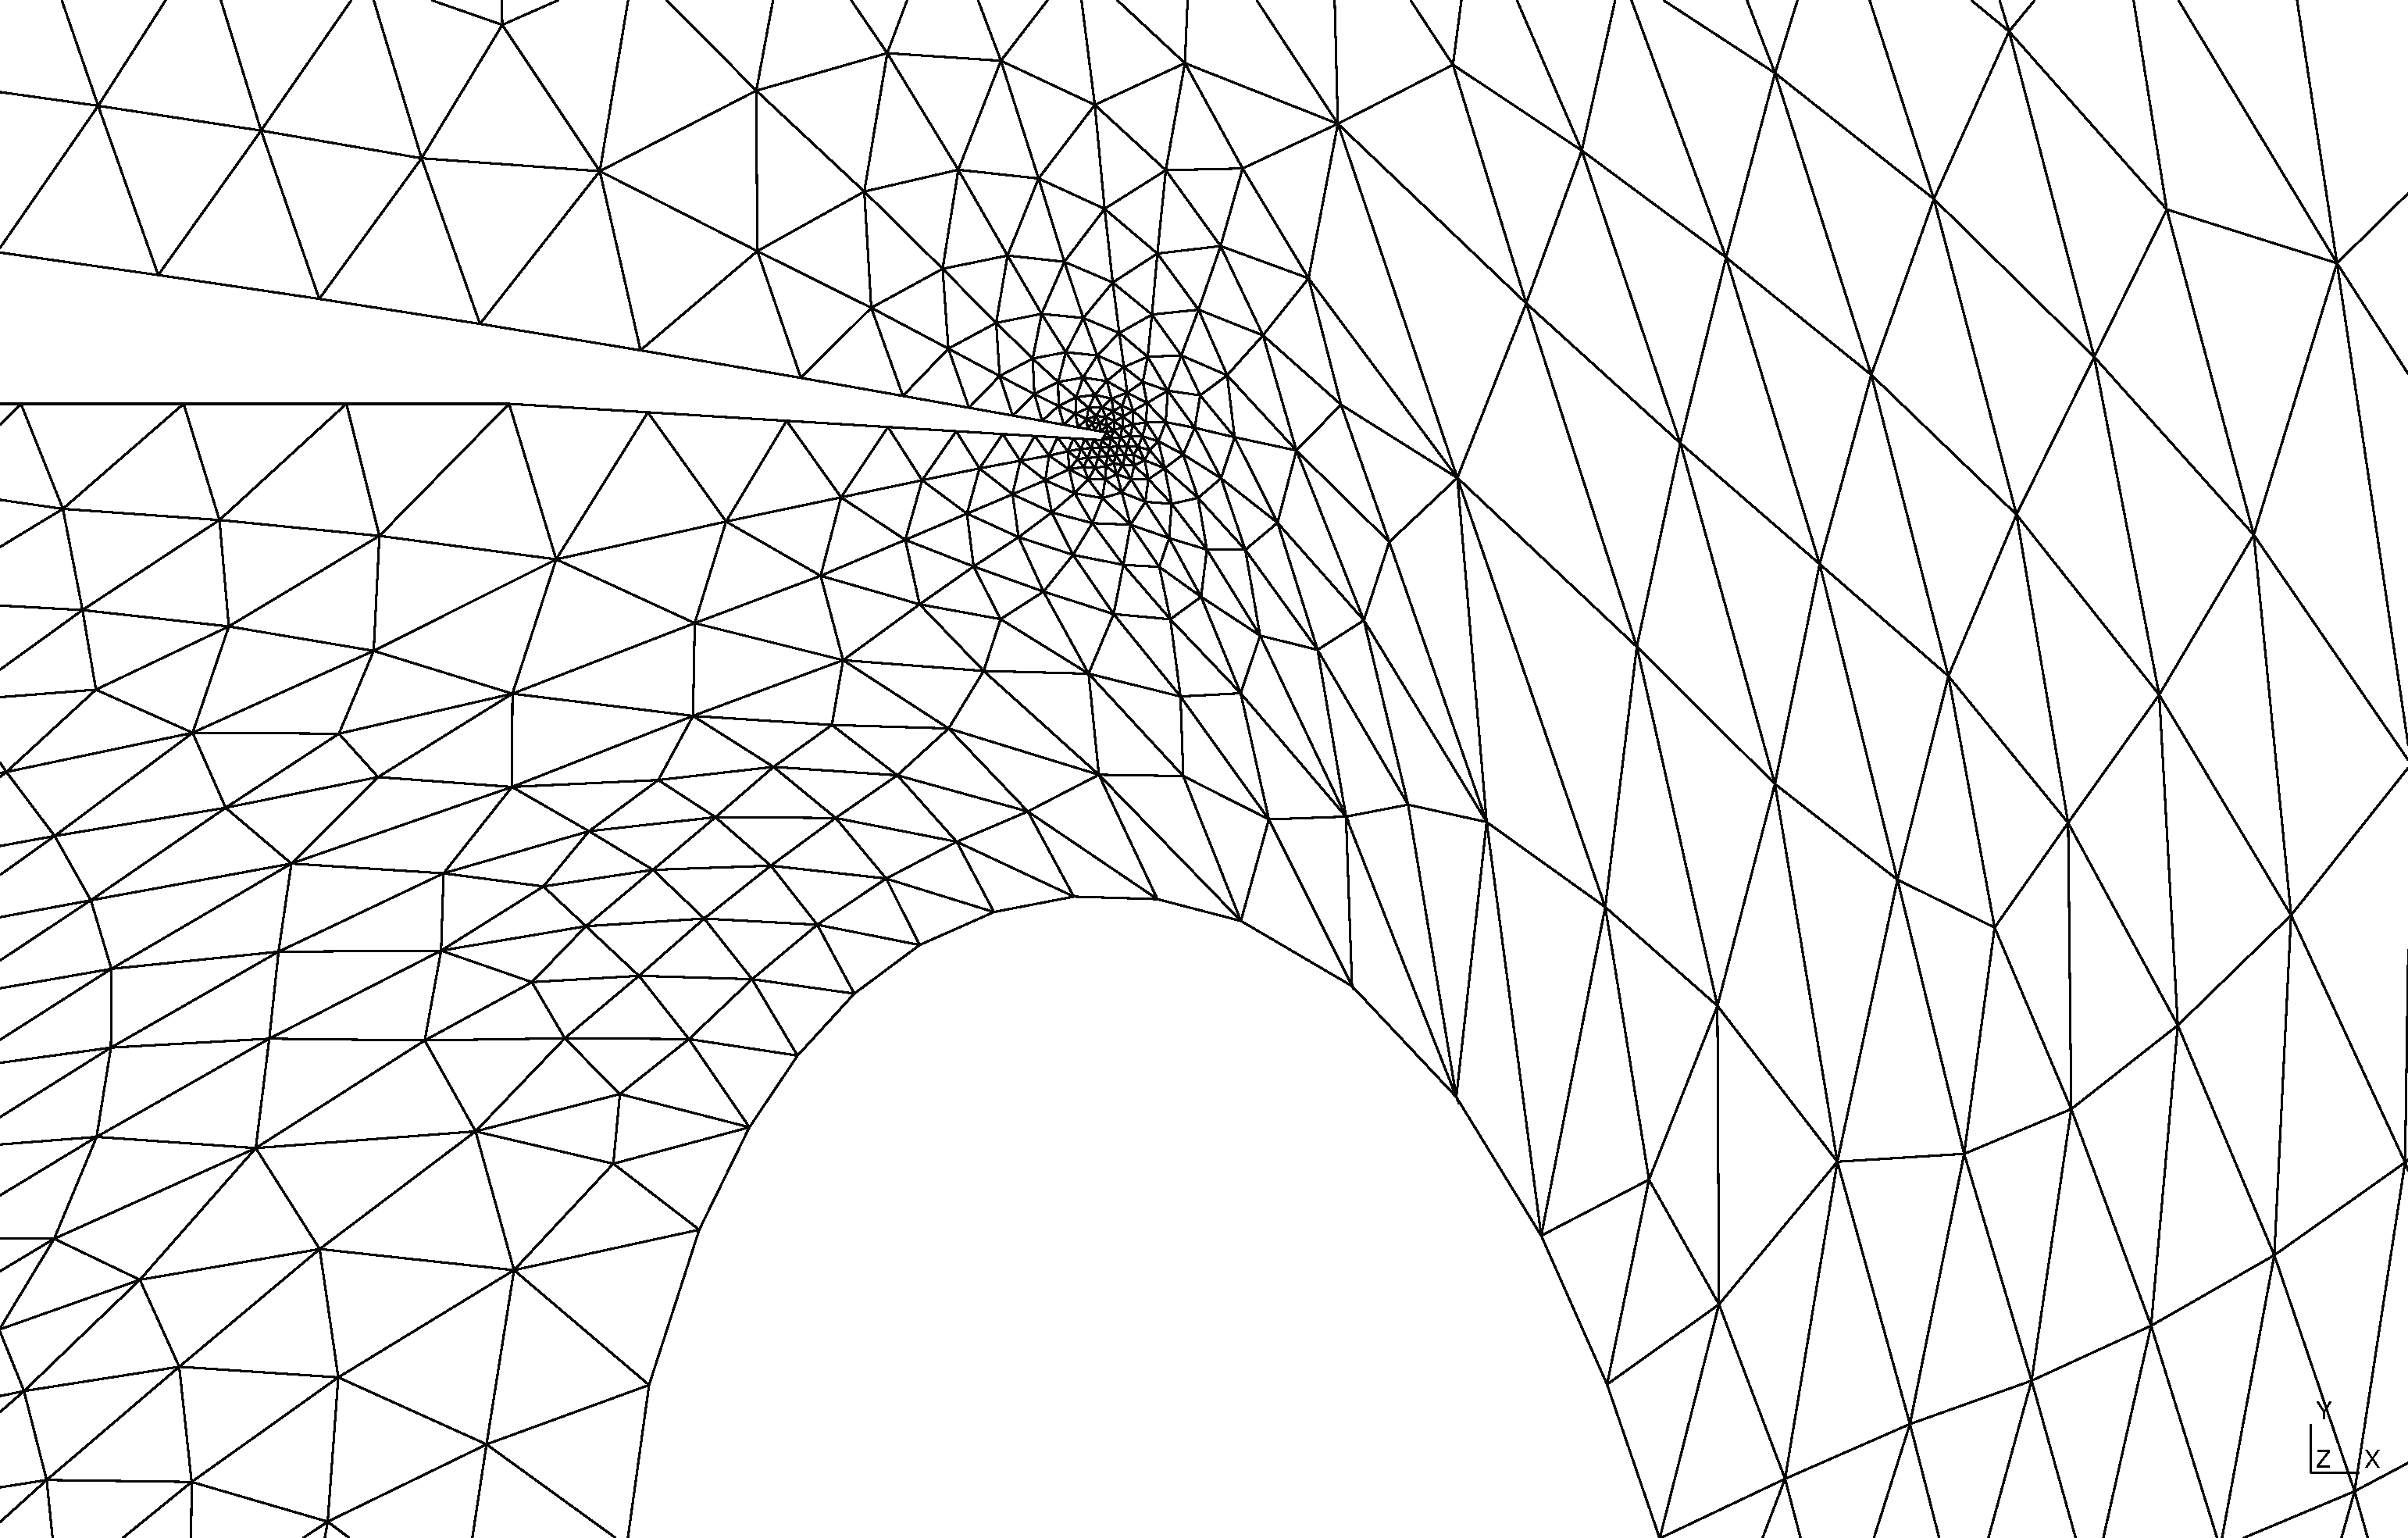
\includegraphics[scale=0.17]{wing60-rbf-sr15-s3_zoomed}
	\caption{Inviscid 3-component airfoil mesh with 60$^\circ$ rotation of flap by RBF method; zoomed to where the flap meets the wing}
	\label{fig:wing-inviscid-rbf-zoomed}
\end{figure}
\end{frame}
\begin{frame}{RBF}
\begin{figure}
	\centering
	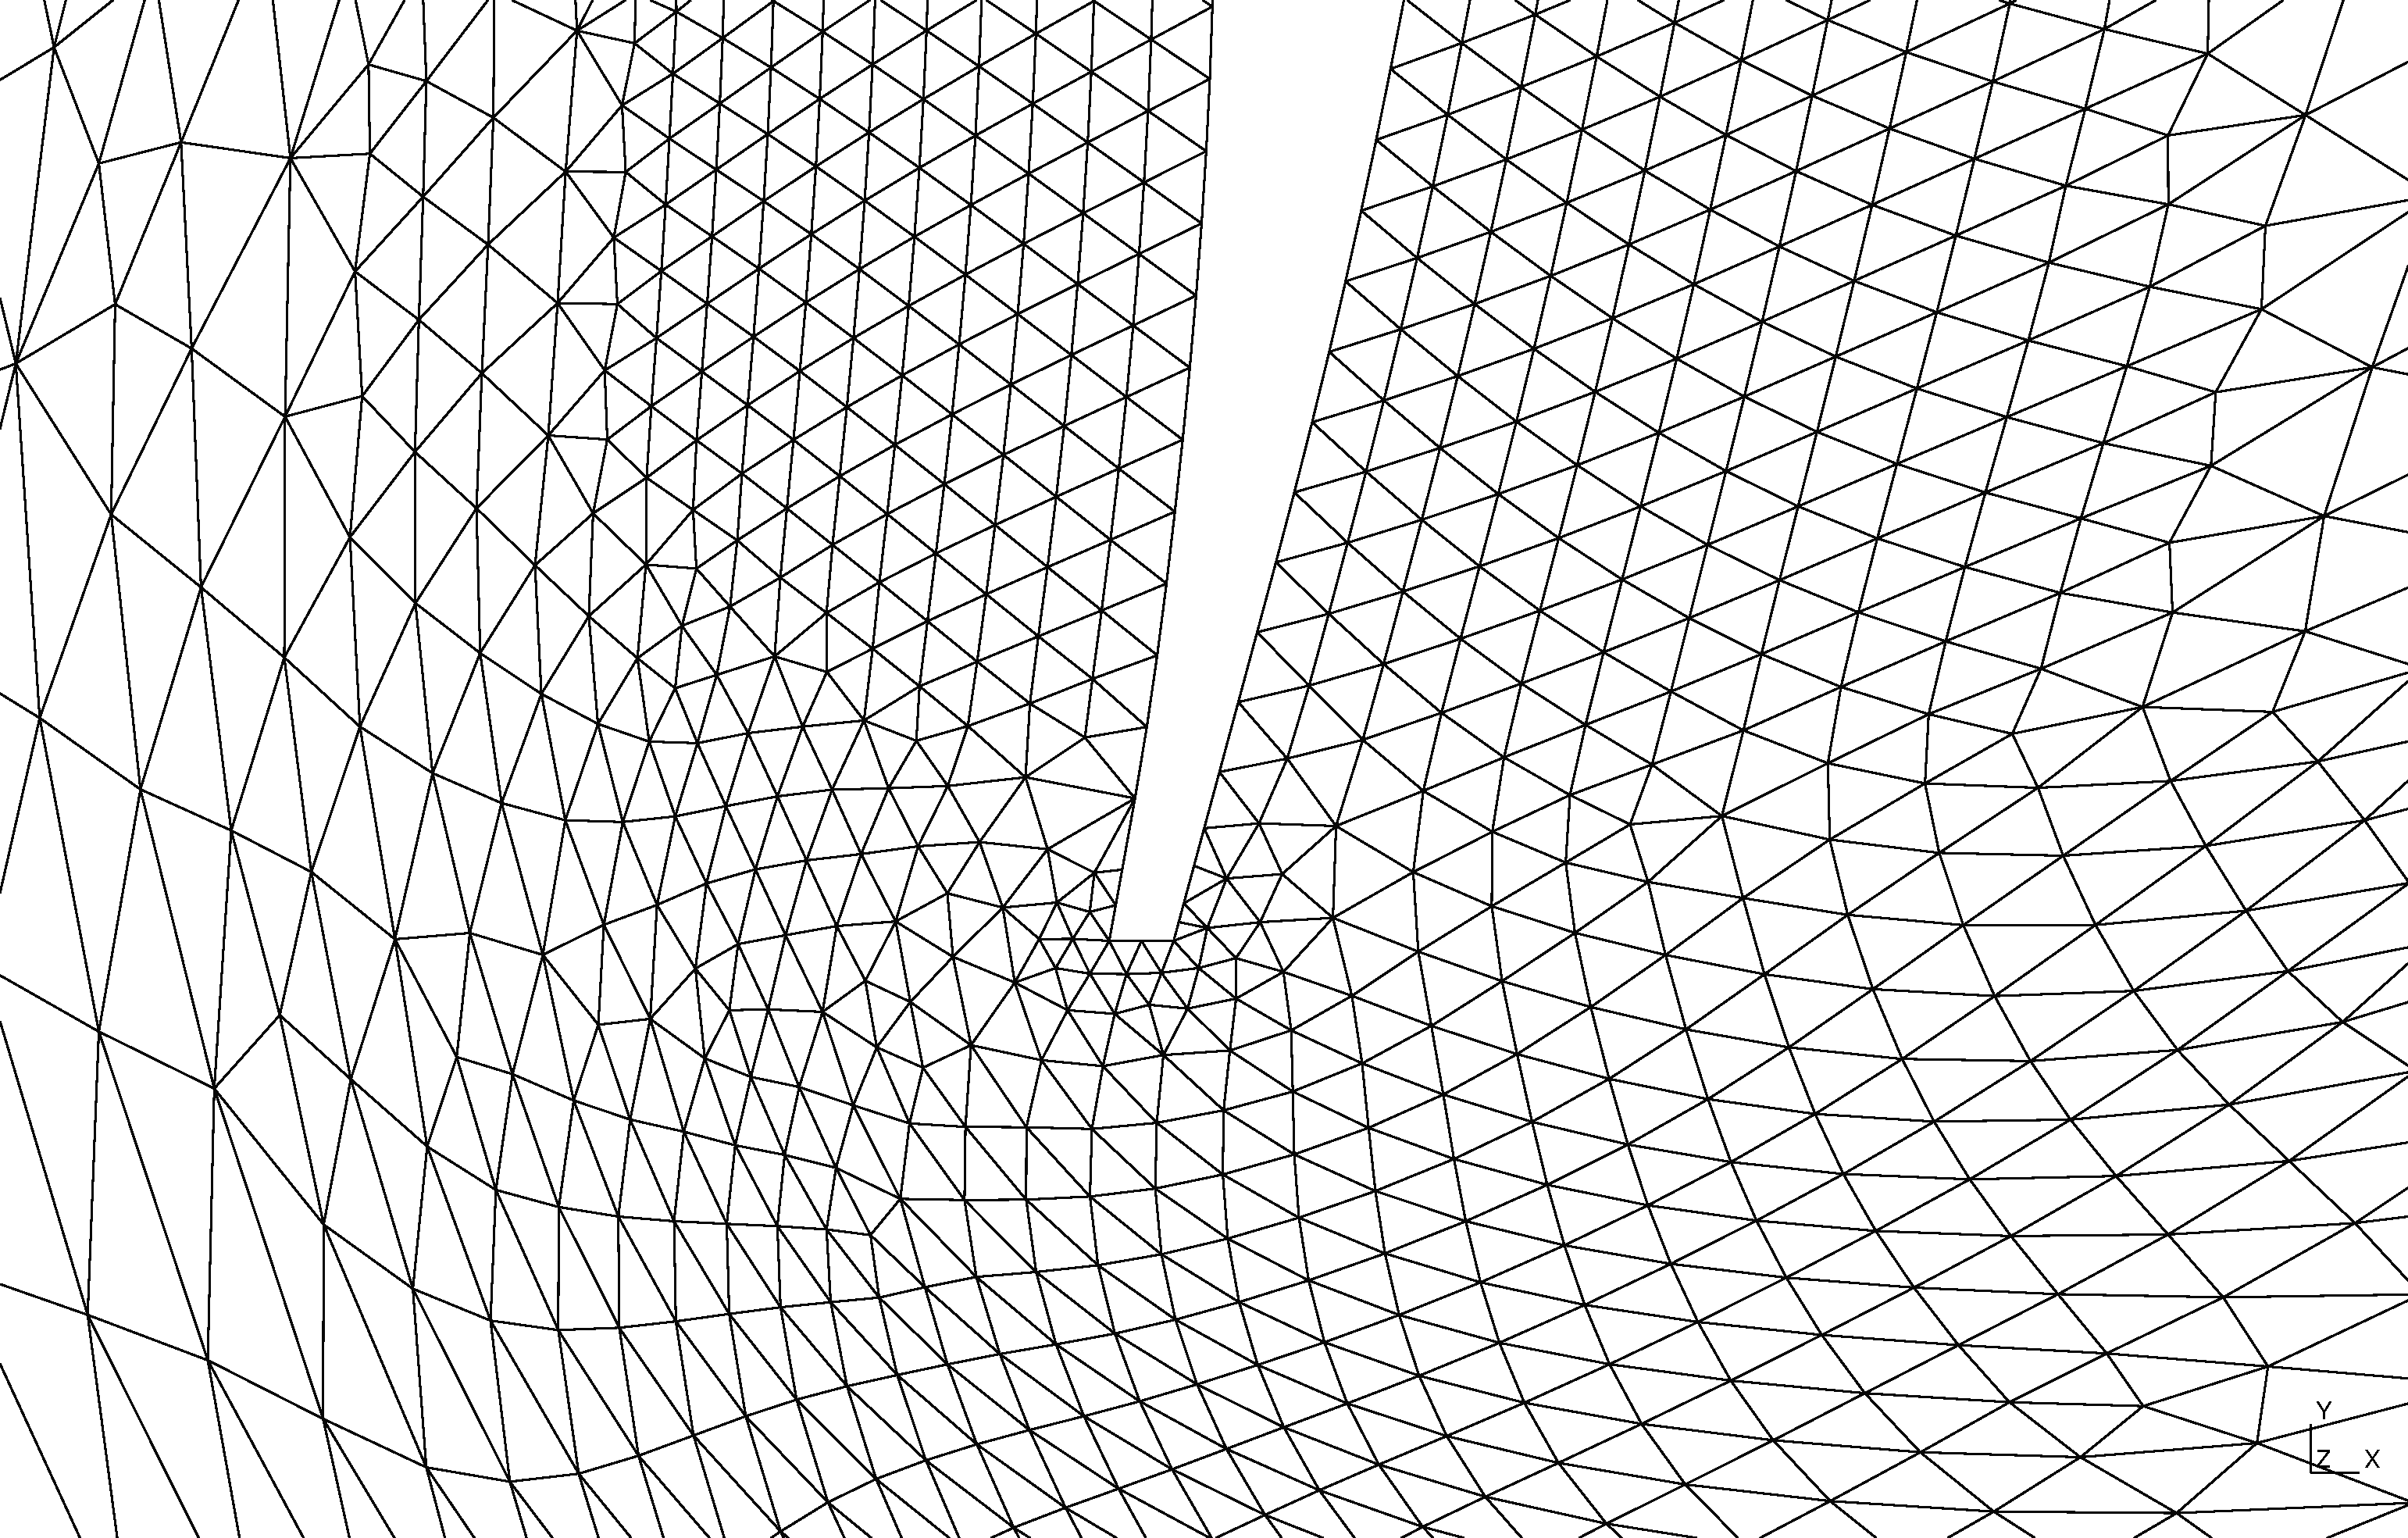
\includegraphics[scale=0.17]{wing60-rbf-sr15-s3_zoomed2}
	\caption{Inviscid 3-component airfoil mesh with 60$^\circ$ rotation of flap by RBF method, zoomed to the trailing edge of the flap}
	\label{fig:wing-inviscid-rbf-zoomed2}
\end{figure}
\end{frame}

\subsection{Mesh quality}
\begin{frame}{Mesh quality metrics}
In order to judge the effectiveness of mesh-movement methods, we need to measure the quality of the deformed mesh.

Some mesh quality measures have been derived for linear 2D and 3D elements by Knupp \footfullcite{qualknupp}: 
\begin{itemize}
\item size 
\item shape 
\item skew 
\item size-shape and size-skew 
\end{itemize}
metrics for triangles, quadrangles, tetrahedra and hexahedra.
\end{frame}

\begin{frame}{Shape metric}
Shape metric takes into account the relative lengths of the edges of a cell, and the relative interior angles of a cell.
 \begin{figure}
 	\centering
 	\subfloat{
 		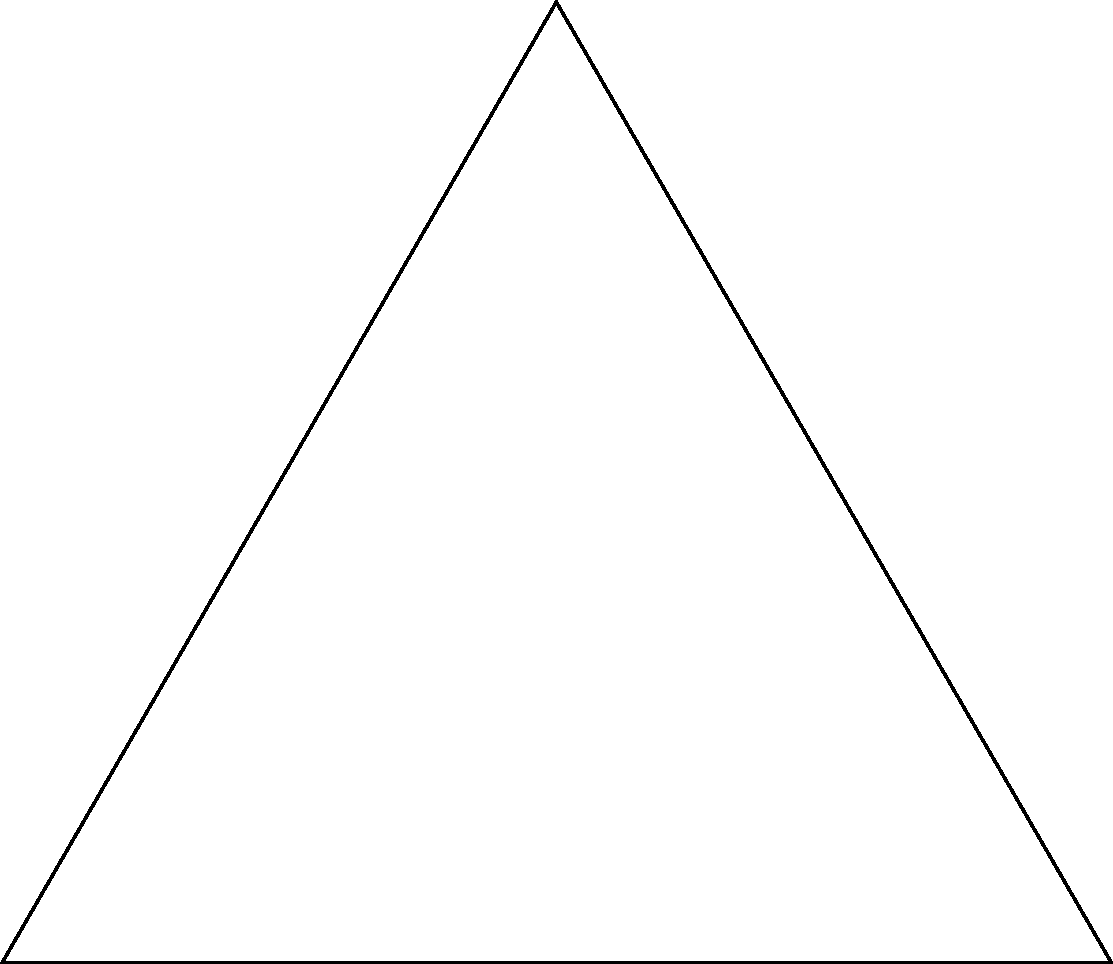
\includegraphics[scale=0.12]{tri_ideal}
 	}
 	\hspace{0.2in}
 	\subfloat{
 		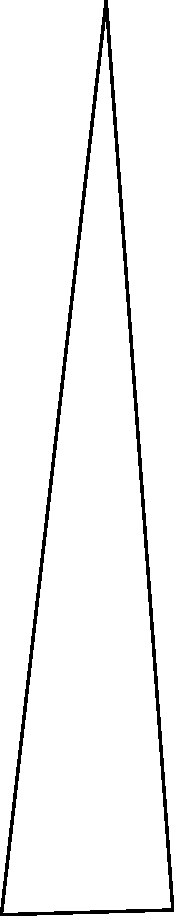
\includegraphics[scale=0.15]{tri_bad}
 	}
 	\hspace{0.2in}
 	\subfloat{
 		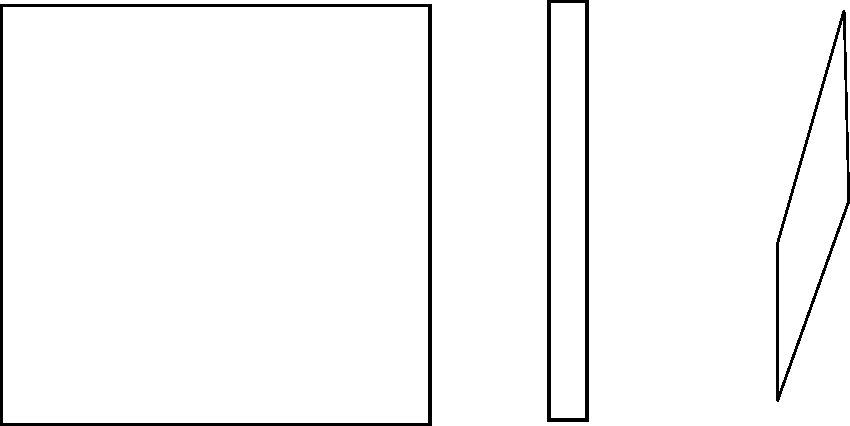
\includegraphics[scale=0.25]{quad_quality}
 	}
 	\caption{Cell shape quality. From left to right: triangle with good shape, triangle with bad shape, quadrilateral with good shape, quadrilateral with bad shape and another quadrilateral with bad shape}
 	\label{fig:shape}
 \end{figure}
\end{frame}

\begin{frame}{Skew Metric}
Skew metric takes into account only the relative angles between edges of a cell. For a triangle, it is equivalent to the shape metric.
\begin{figure}
	\centering
	\subfloat{
		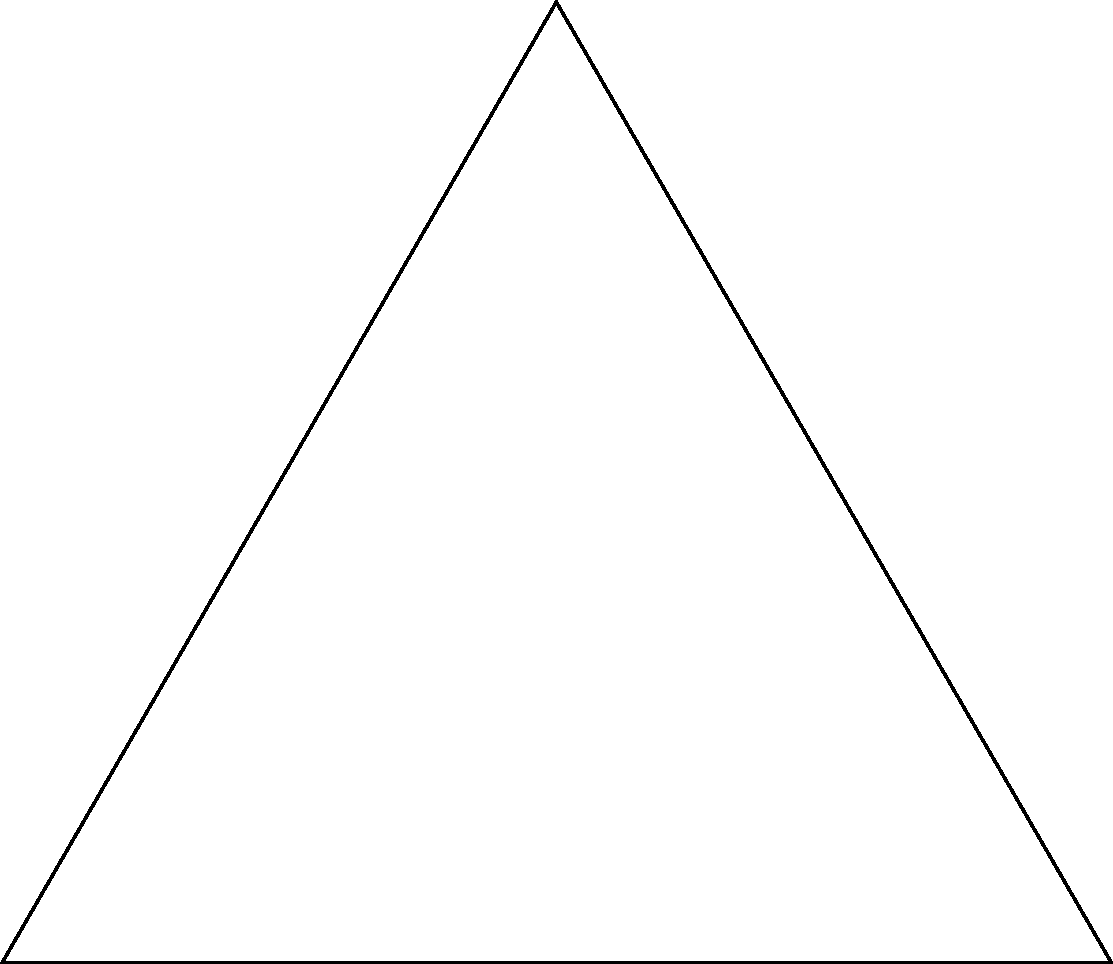
\includegraphics[scale=0.12]{tri_ideal}
	}
	\hspace{0.2in}
	\subfloat{
		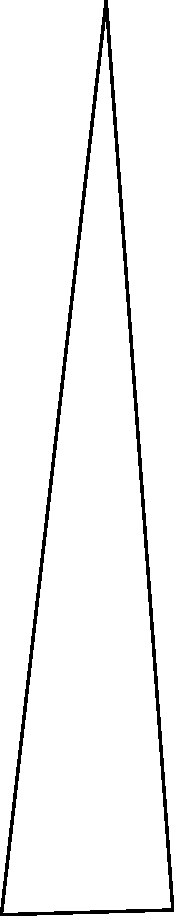
\includegraphics[scale=0.15]{tri_bad}
	}
	\hspace{0.2in}
	\subfloat{
		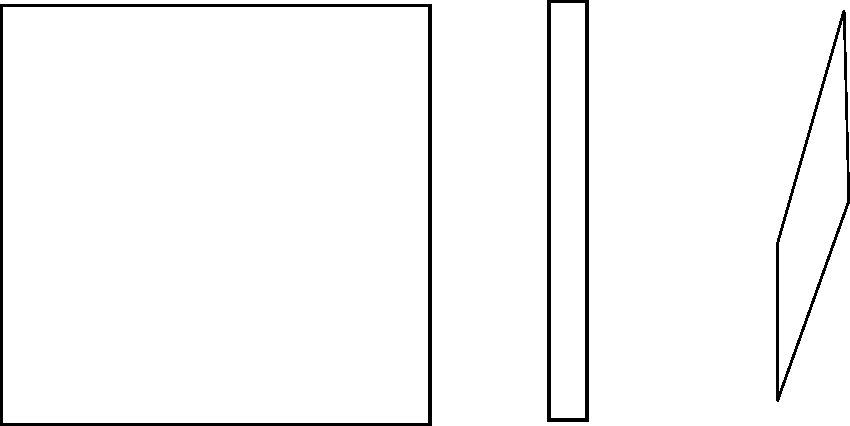
\includegraphics[scale=0.27]{quad_quality}
	}
	\caption{Cell skew quality. From left to right: good triangle, bad triangle, good quadrilateral, \emph{good} quadrilateral (but with bad shape) and a quadrilateral with both bad skew and bad shape qualities}
	\label{fig:skew}
\end{figure}
\end{frame}

\begin{frame}{Mesh quality metrics}
Shape quality:
\begin{align}
f_{shape} &= \frac{\sqrt{3}r\sin\theta}{1-r\cos\theta+r^2} \text{ for triangles} \\
f_{shape} &= \frac{8}{\sum_0^3(1+r_k^2)/(r_k\sin\theta_k)} \text{ for quads.}
\end{align}
Skew quality for quadrilaterals:
\begin{equation}
f_{skew} = \frac{4}{\sum_0^3 1/\sin\theta_k}.
\end{equation}
$r$ is the ratio of consecutive edge lengths.

We choose to use the shape metric for triangles and the \emph{skew} metric for quadrilaterals.
\end{frame}

\subsection{Large rotation with mesh quality}

\begin{frame}{Comparison of interpolation methods}
 \begin{figure}
 	\centering
 	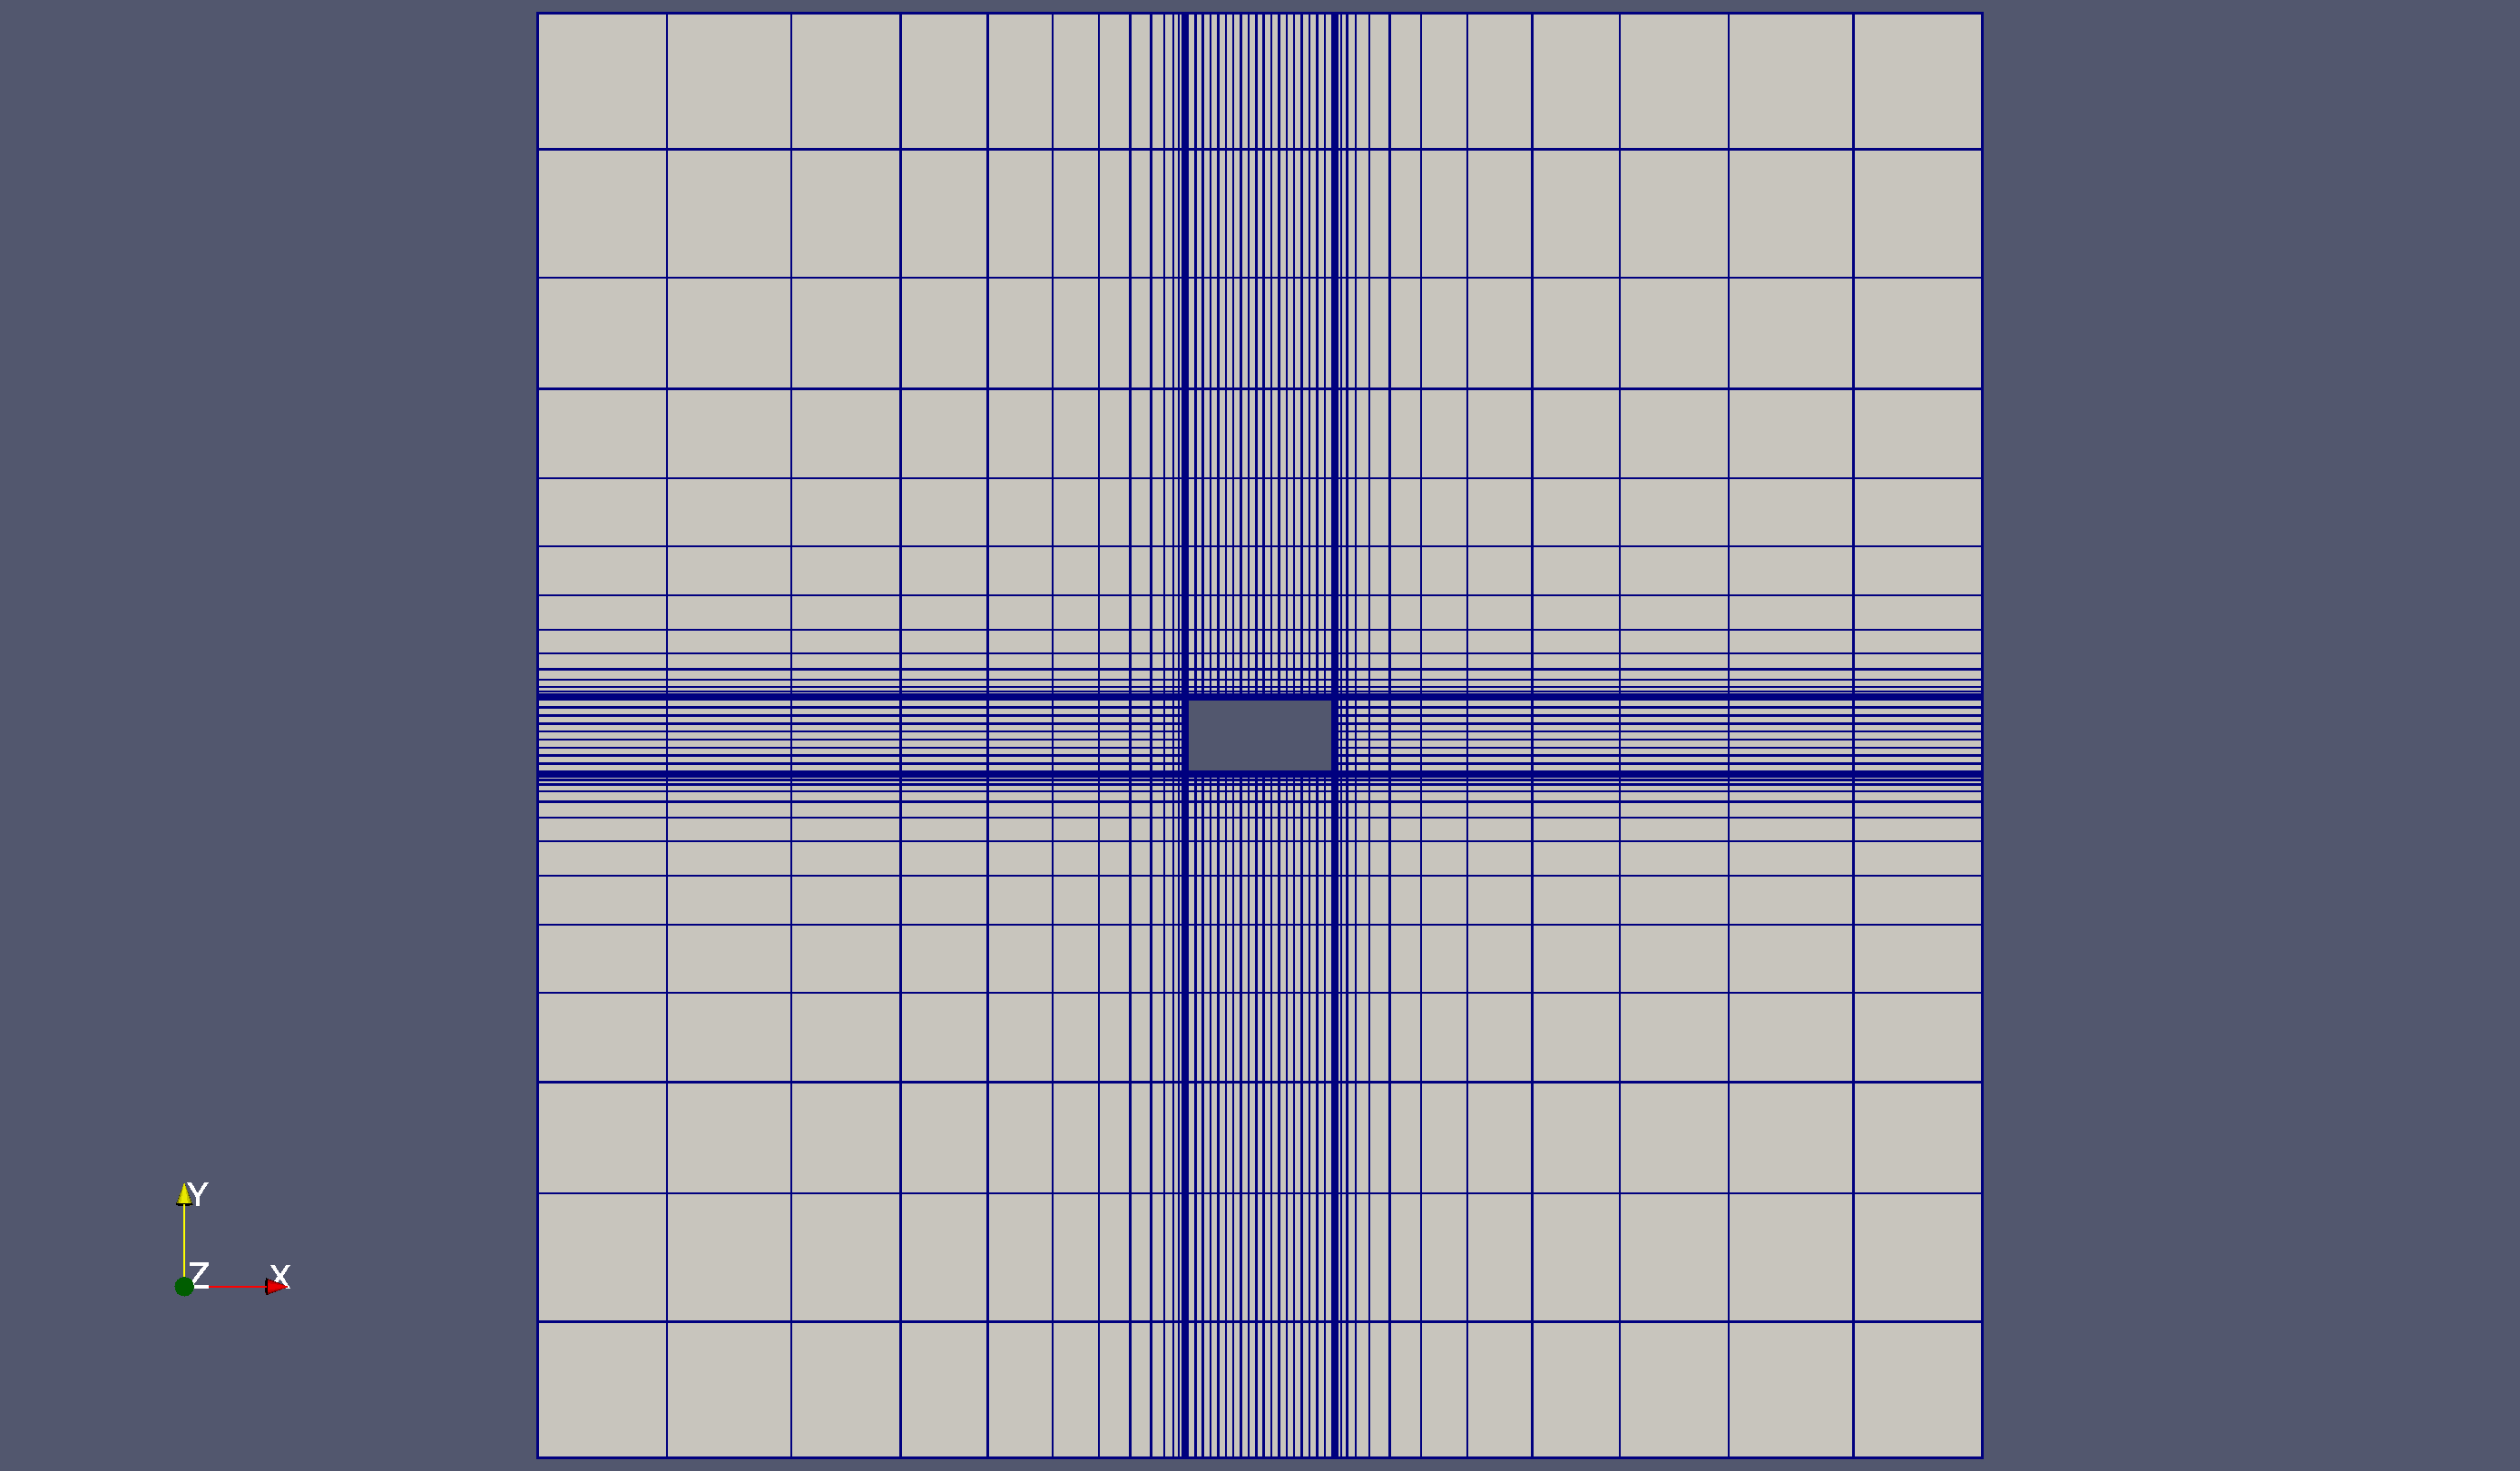
\includegraphics[scale=0.15]{qin-orig-mesh.pdf}
 	\caption{Original mesh}
 	\label{fig:qin-orig}
 \end{figure}
 This test case is taken from Wang \emph{et. al.}\footfullcite{mm:dgrbf}.
\end{frame}
\begin{frame}
	 \begin{figure}
	 	\centering
	 	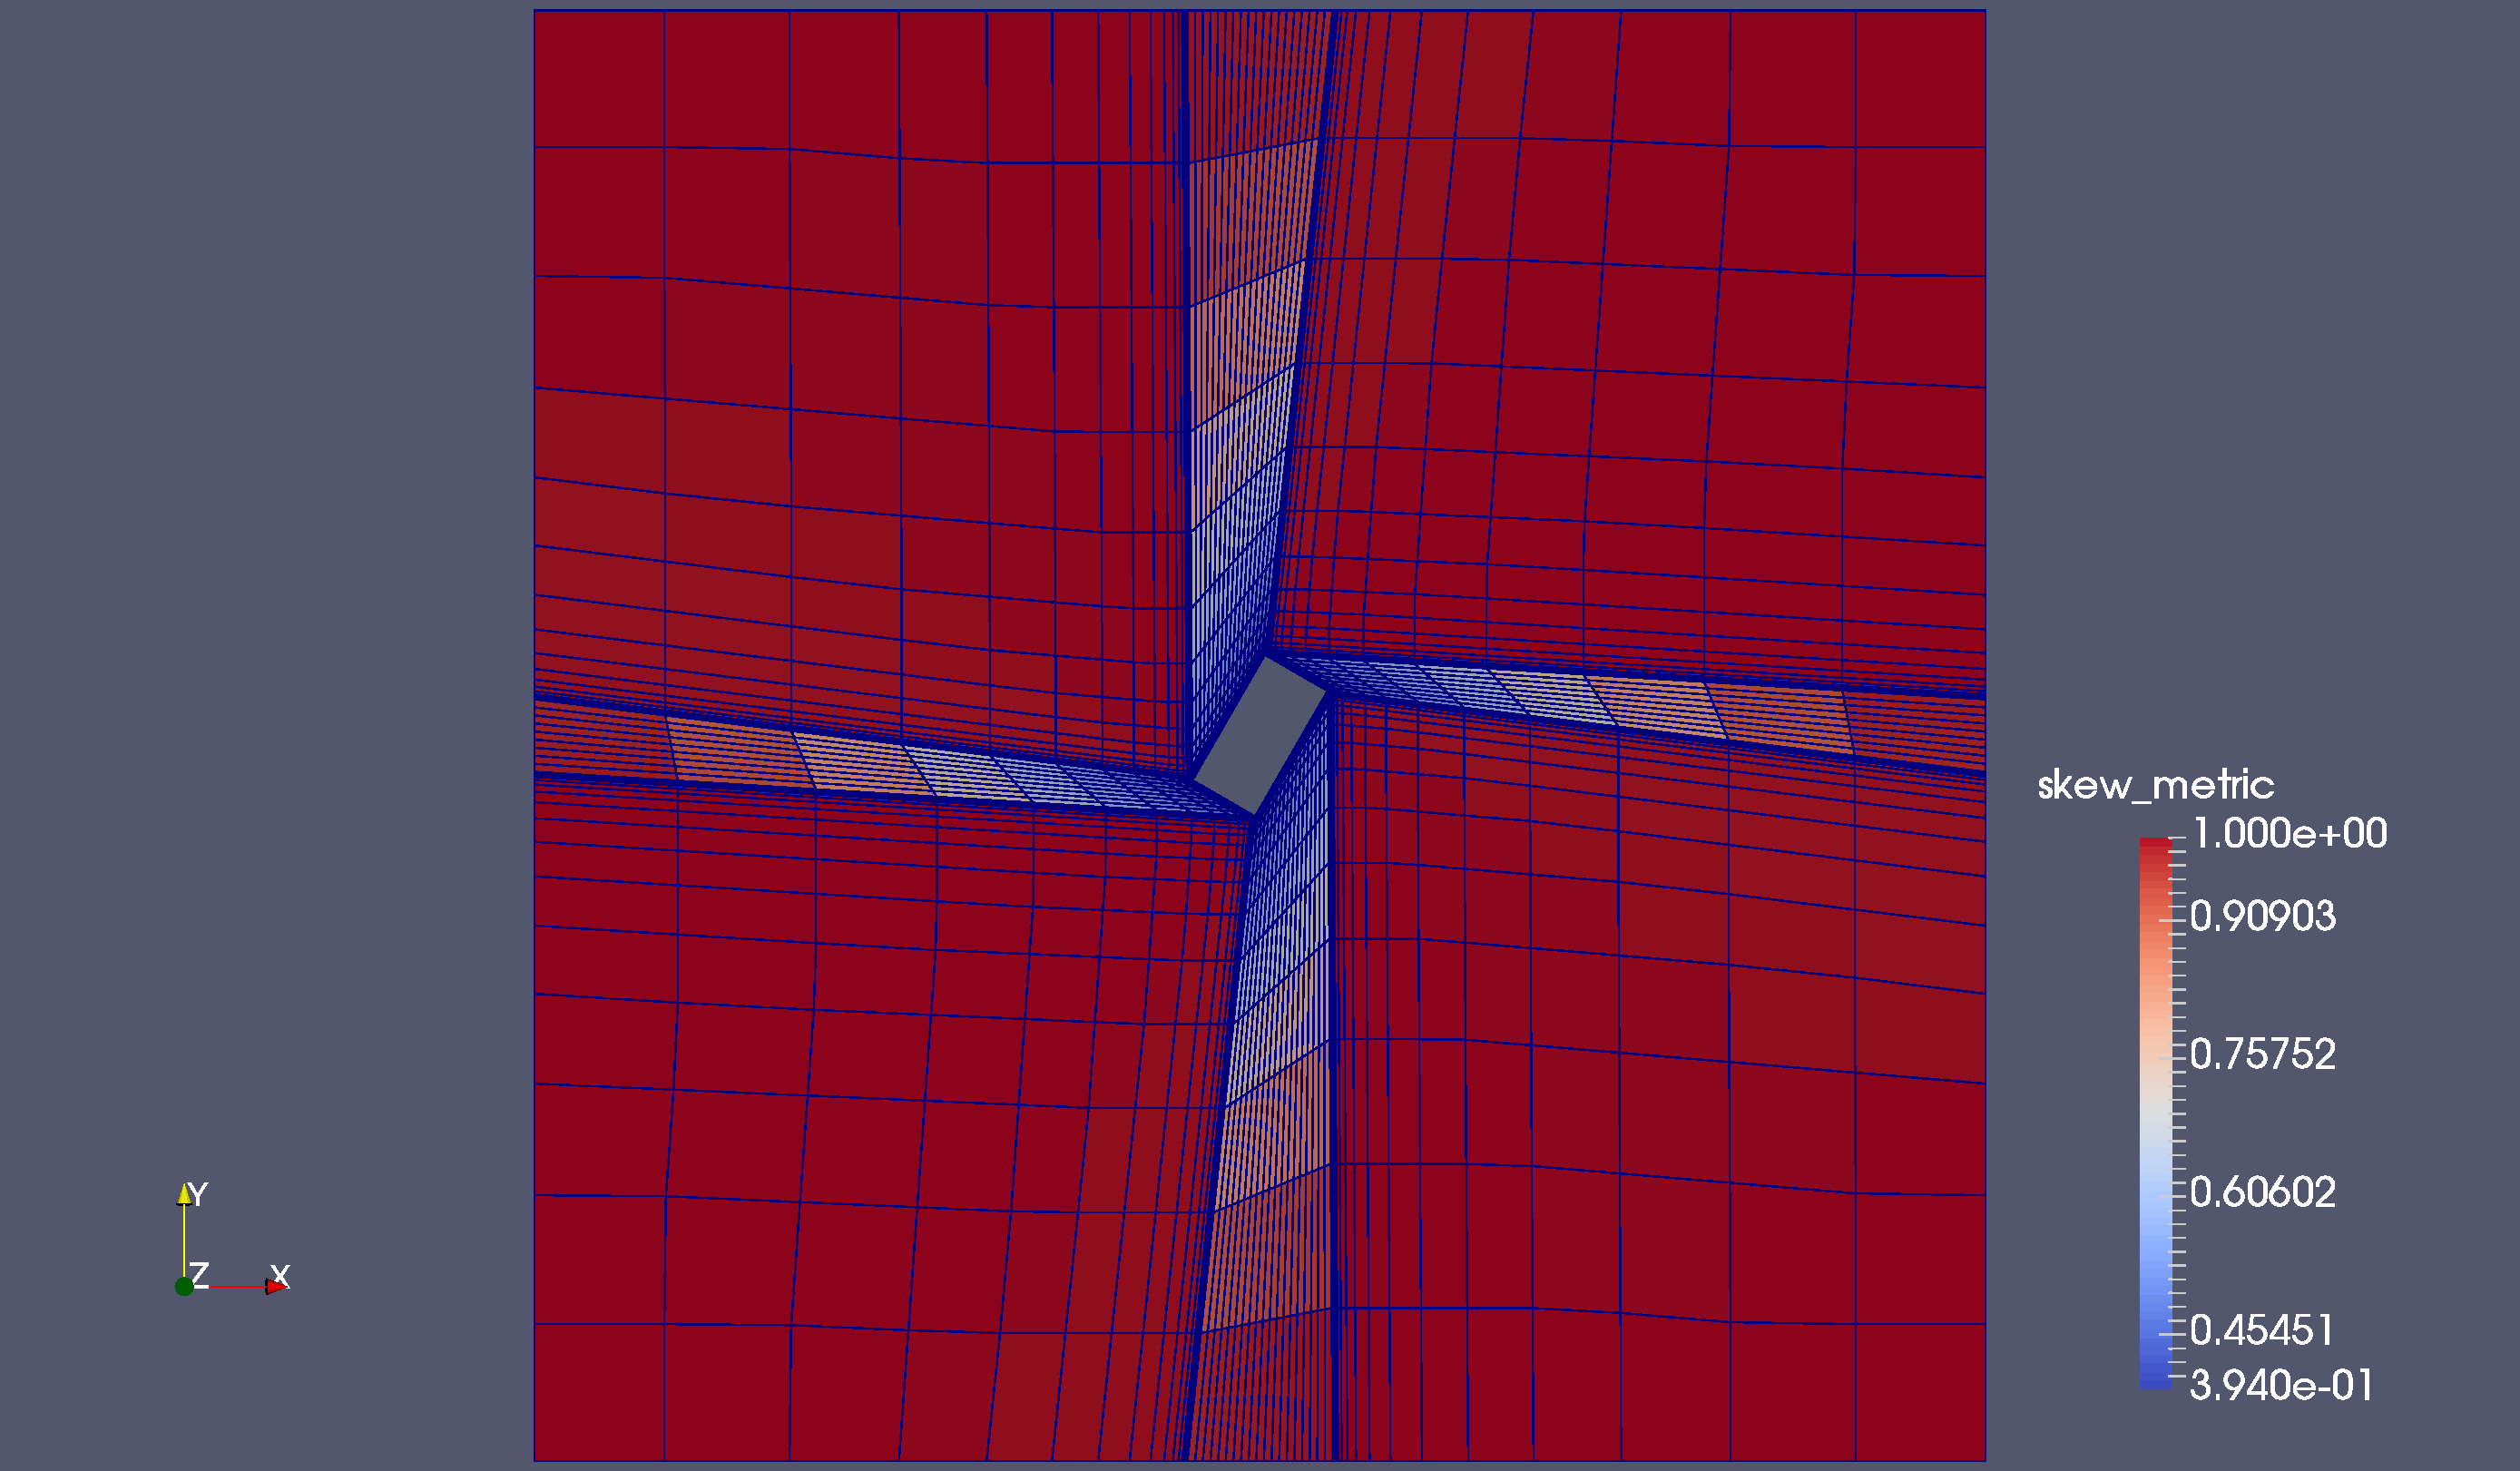
\includegraphics[scale=0.2]{qin-60-dgm-quality.pdf}
	 	\caption{60 degrees rotation by DGM}
	 	\label{fig:qin-60-dgm}
	 \end{figure}
\end{frame}
\begin{frame}
	 \begin{figure}
	 	\centering
	 	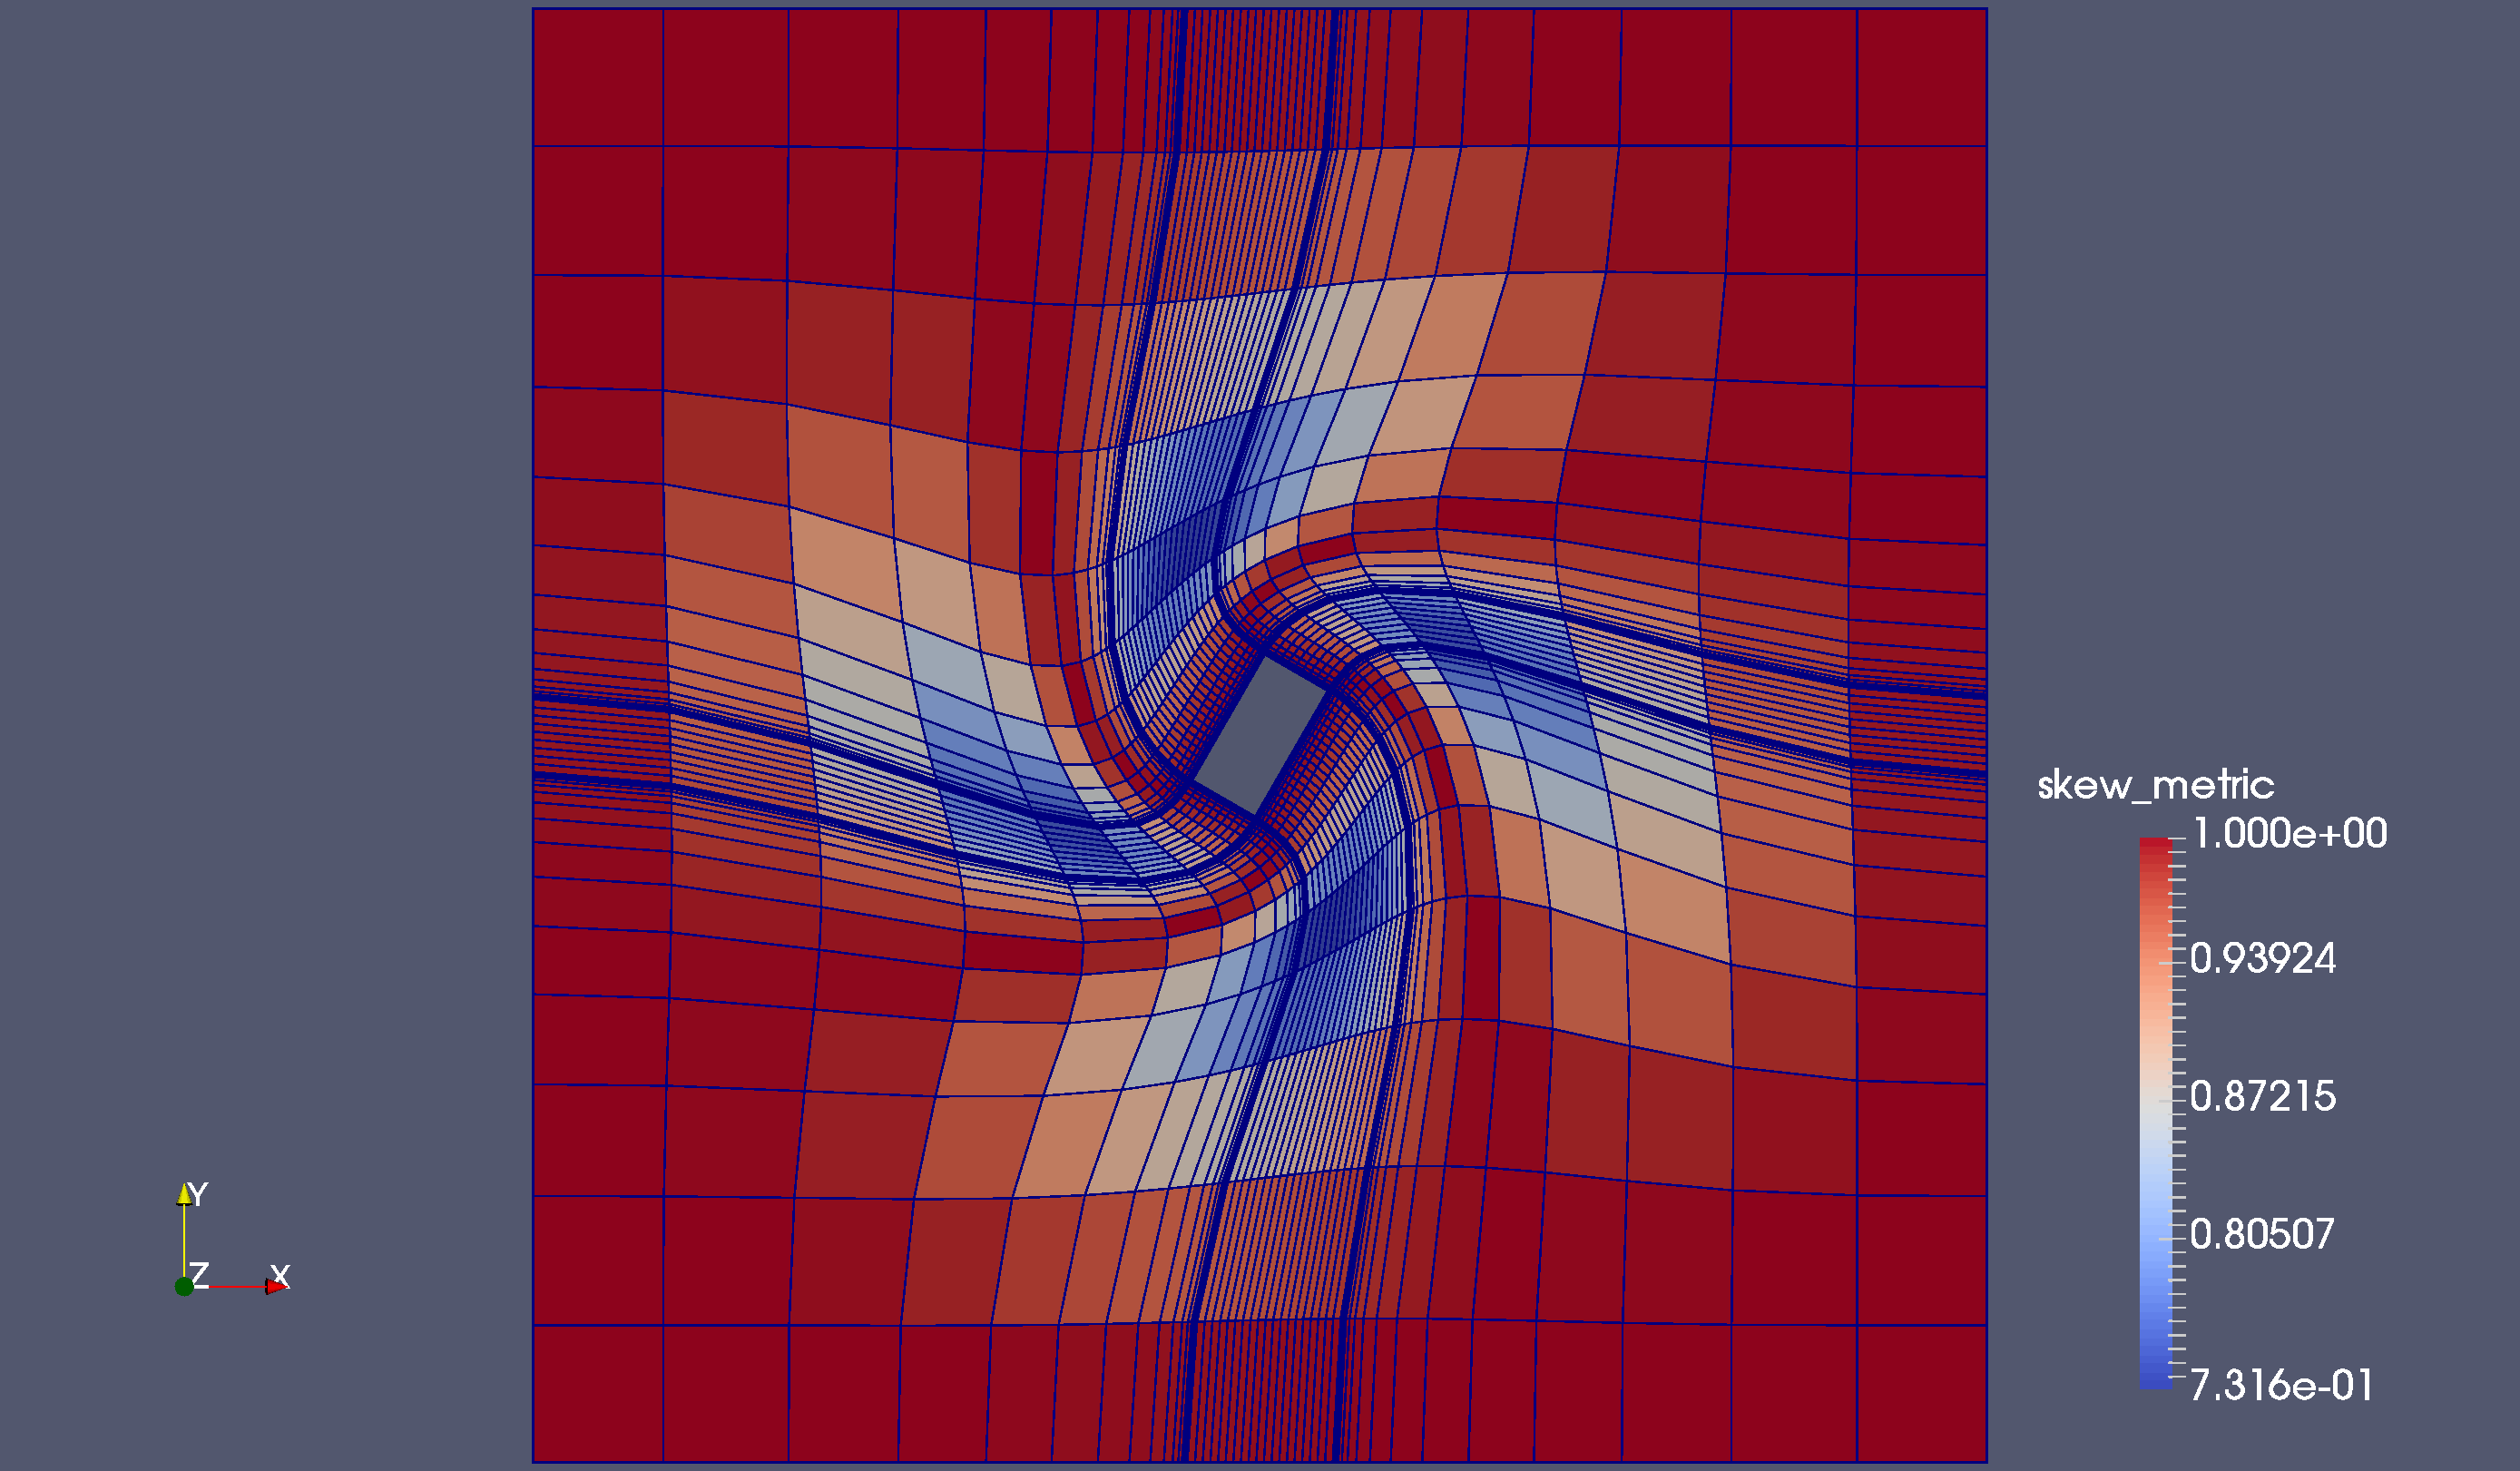
\includegraphics[scale=0.2]{qin-60-rbf-quality.pdf}
	 	\caption{60 degrees rotation by RBF}
	 	\label{fig:qin-60-rbf}
	 \end{figure}
\end{frame}
\begin{frame}
	 \begin{figure}
	 	\centering
	 	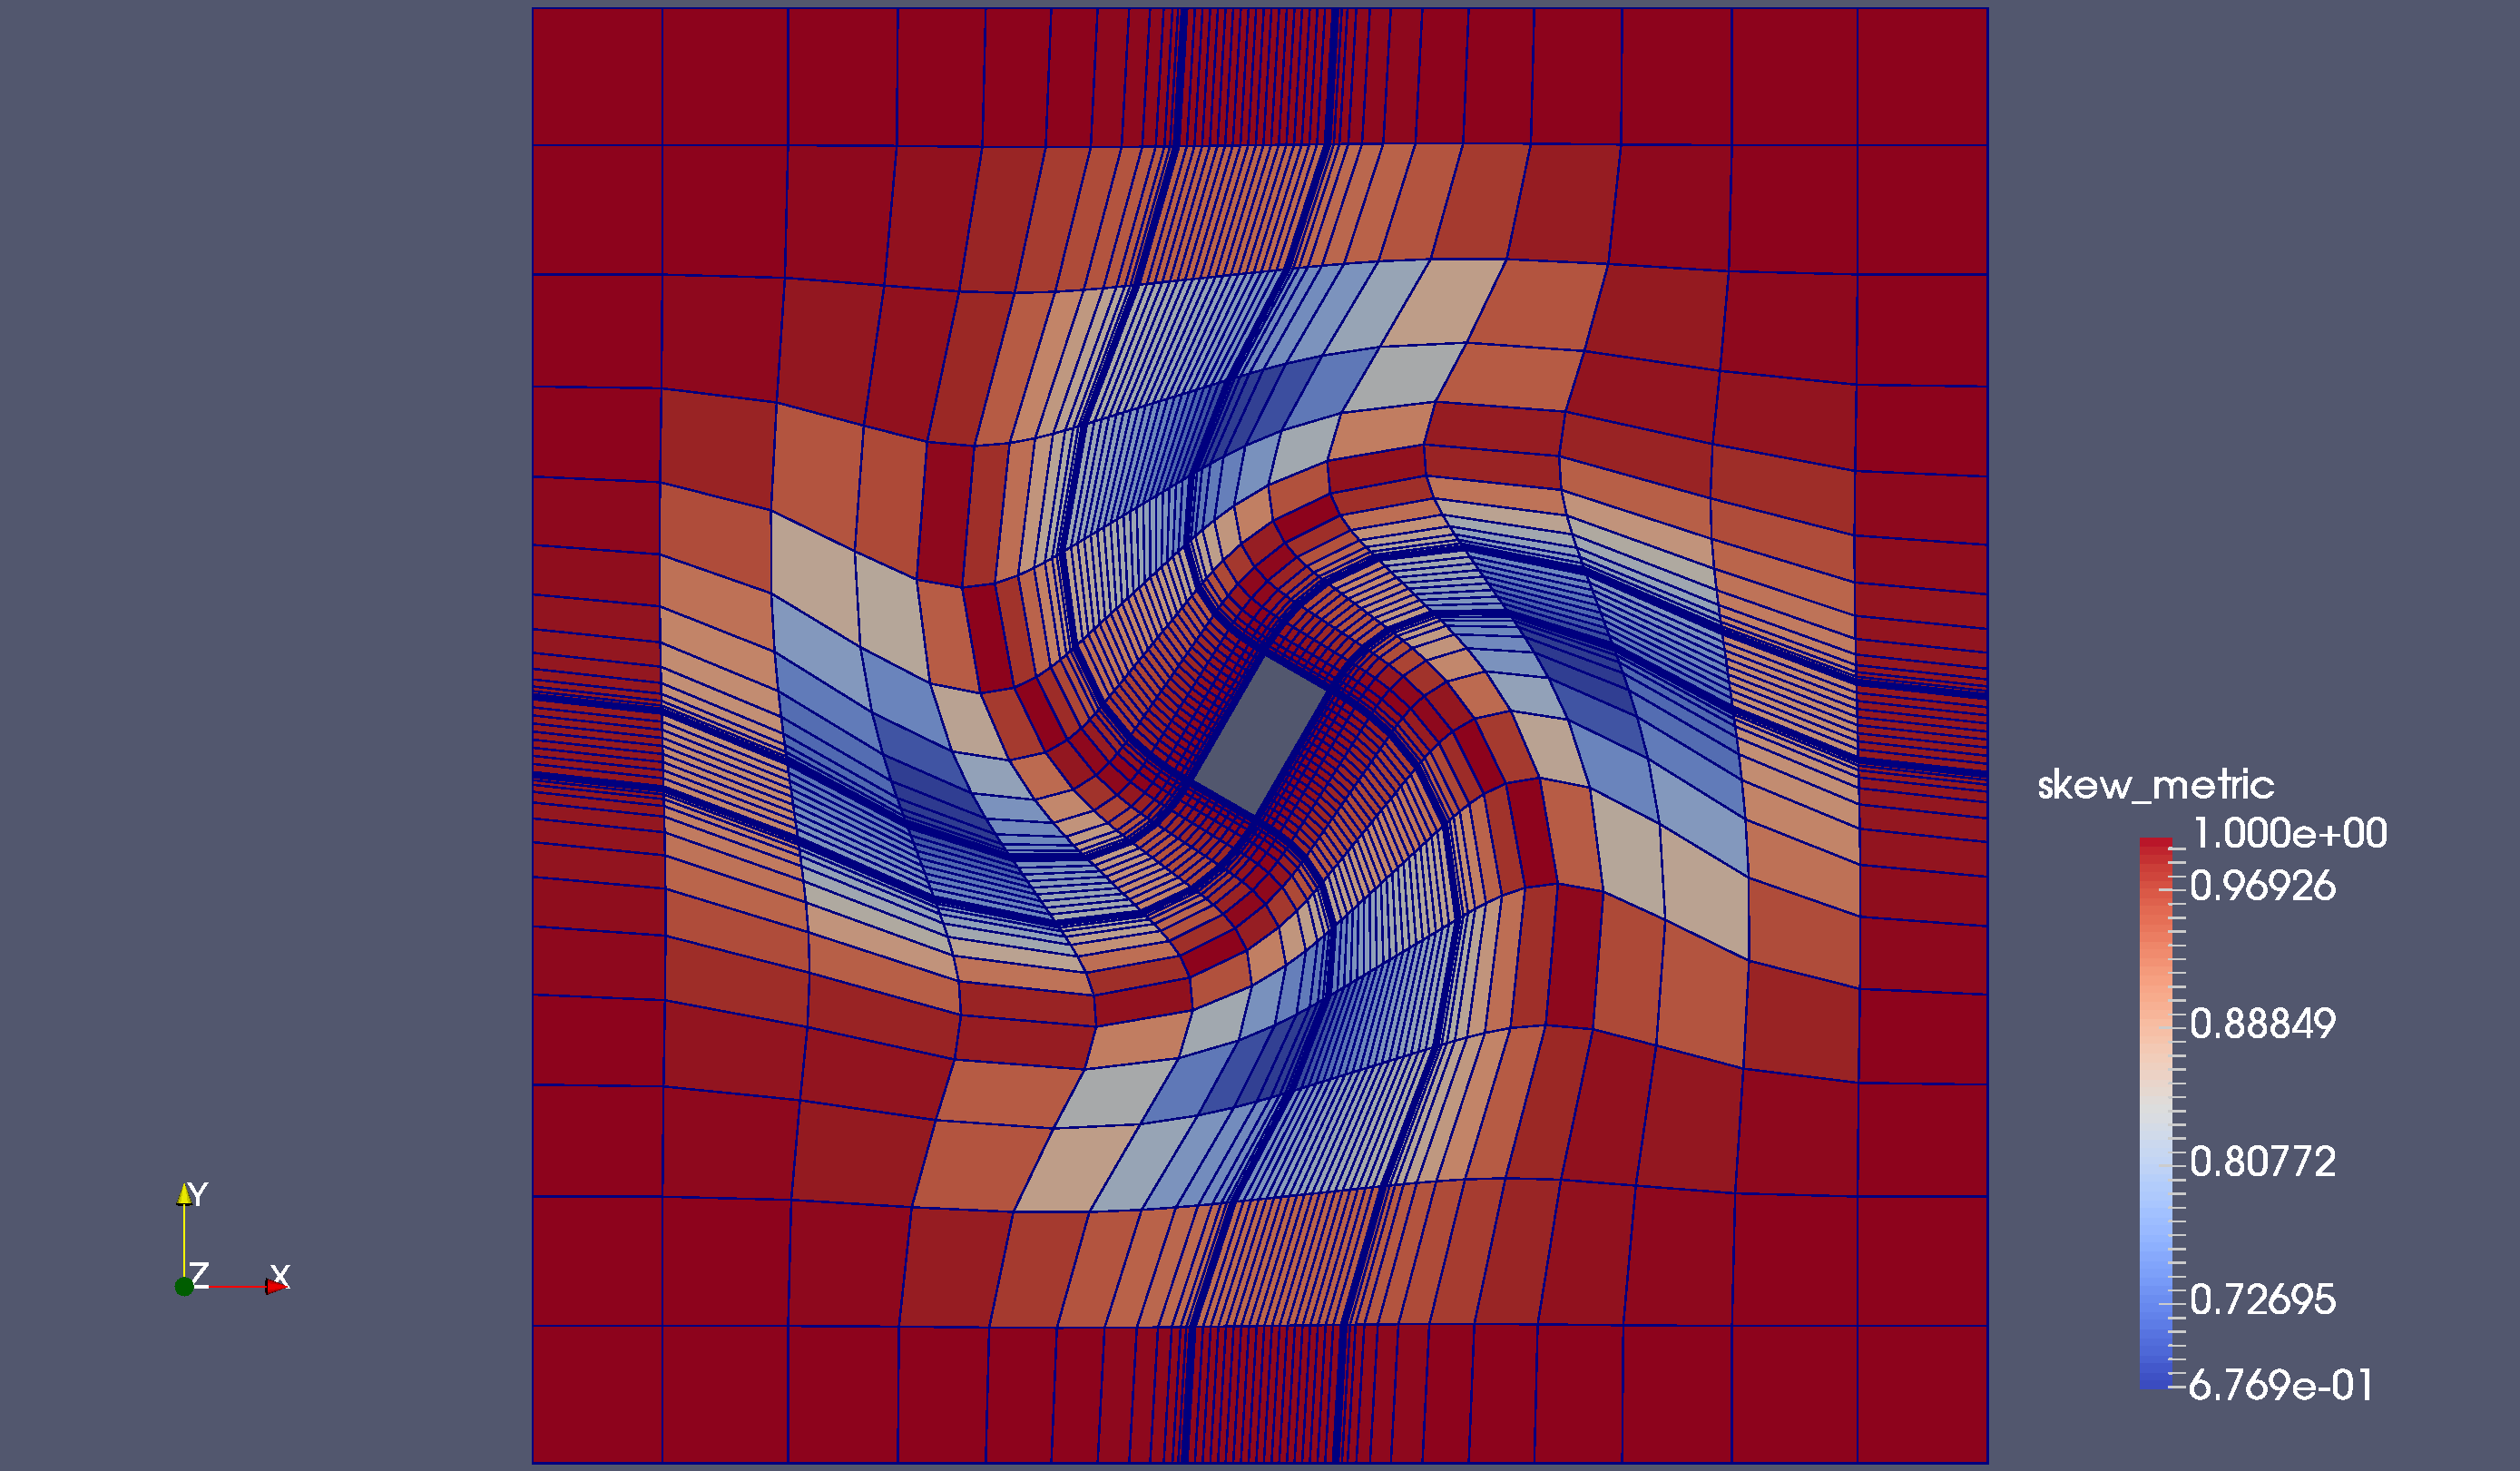
\includegraphics[scale=0.2]{qin-60-dgrbf2-quality.pdf}
	 	\caption{60 degrees rotation by DGRBF2}
	 	\label{fig:qin-60-dgrbf2}
	 \end{figure}
\end{frame}

\begin{frame}{Performance}
	\begin{table}[h!]
		\centering
		\begin{tabular}{|c|c|}
			\hline
			Method & Wall-clock time \\
			\hline
			RBF   &   1.926 s \\
			DGRBF2 &  0.08 s \\
			\hline
		\end{tabular}
		\caption{Performance comparison between RBF and DGRBF2 methods}
	\end{table}
\end{frame}

\begin{frame}
	\begin{figure}
		\centering
		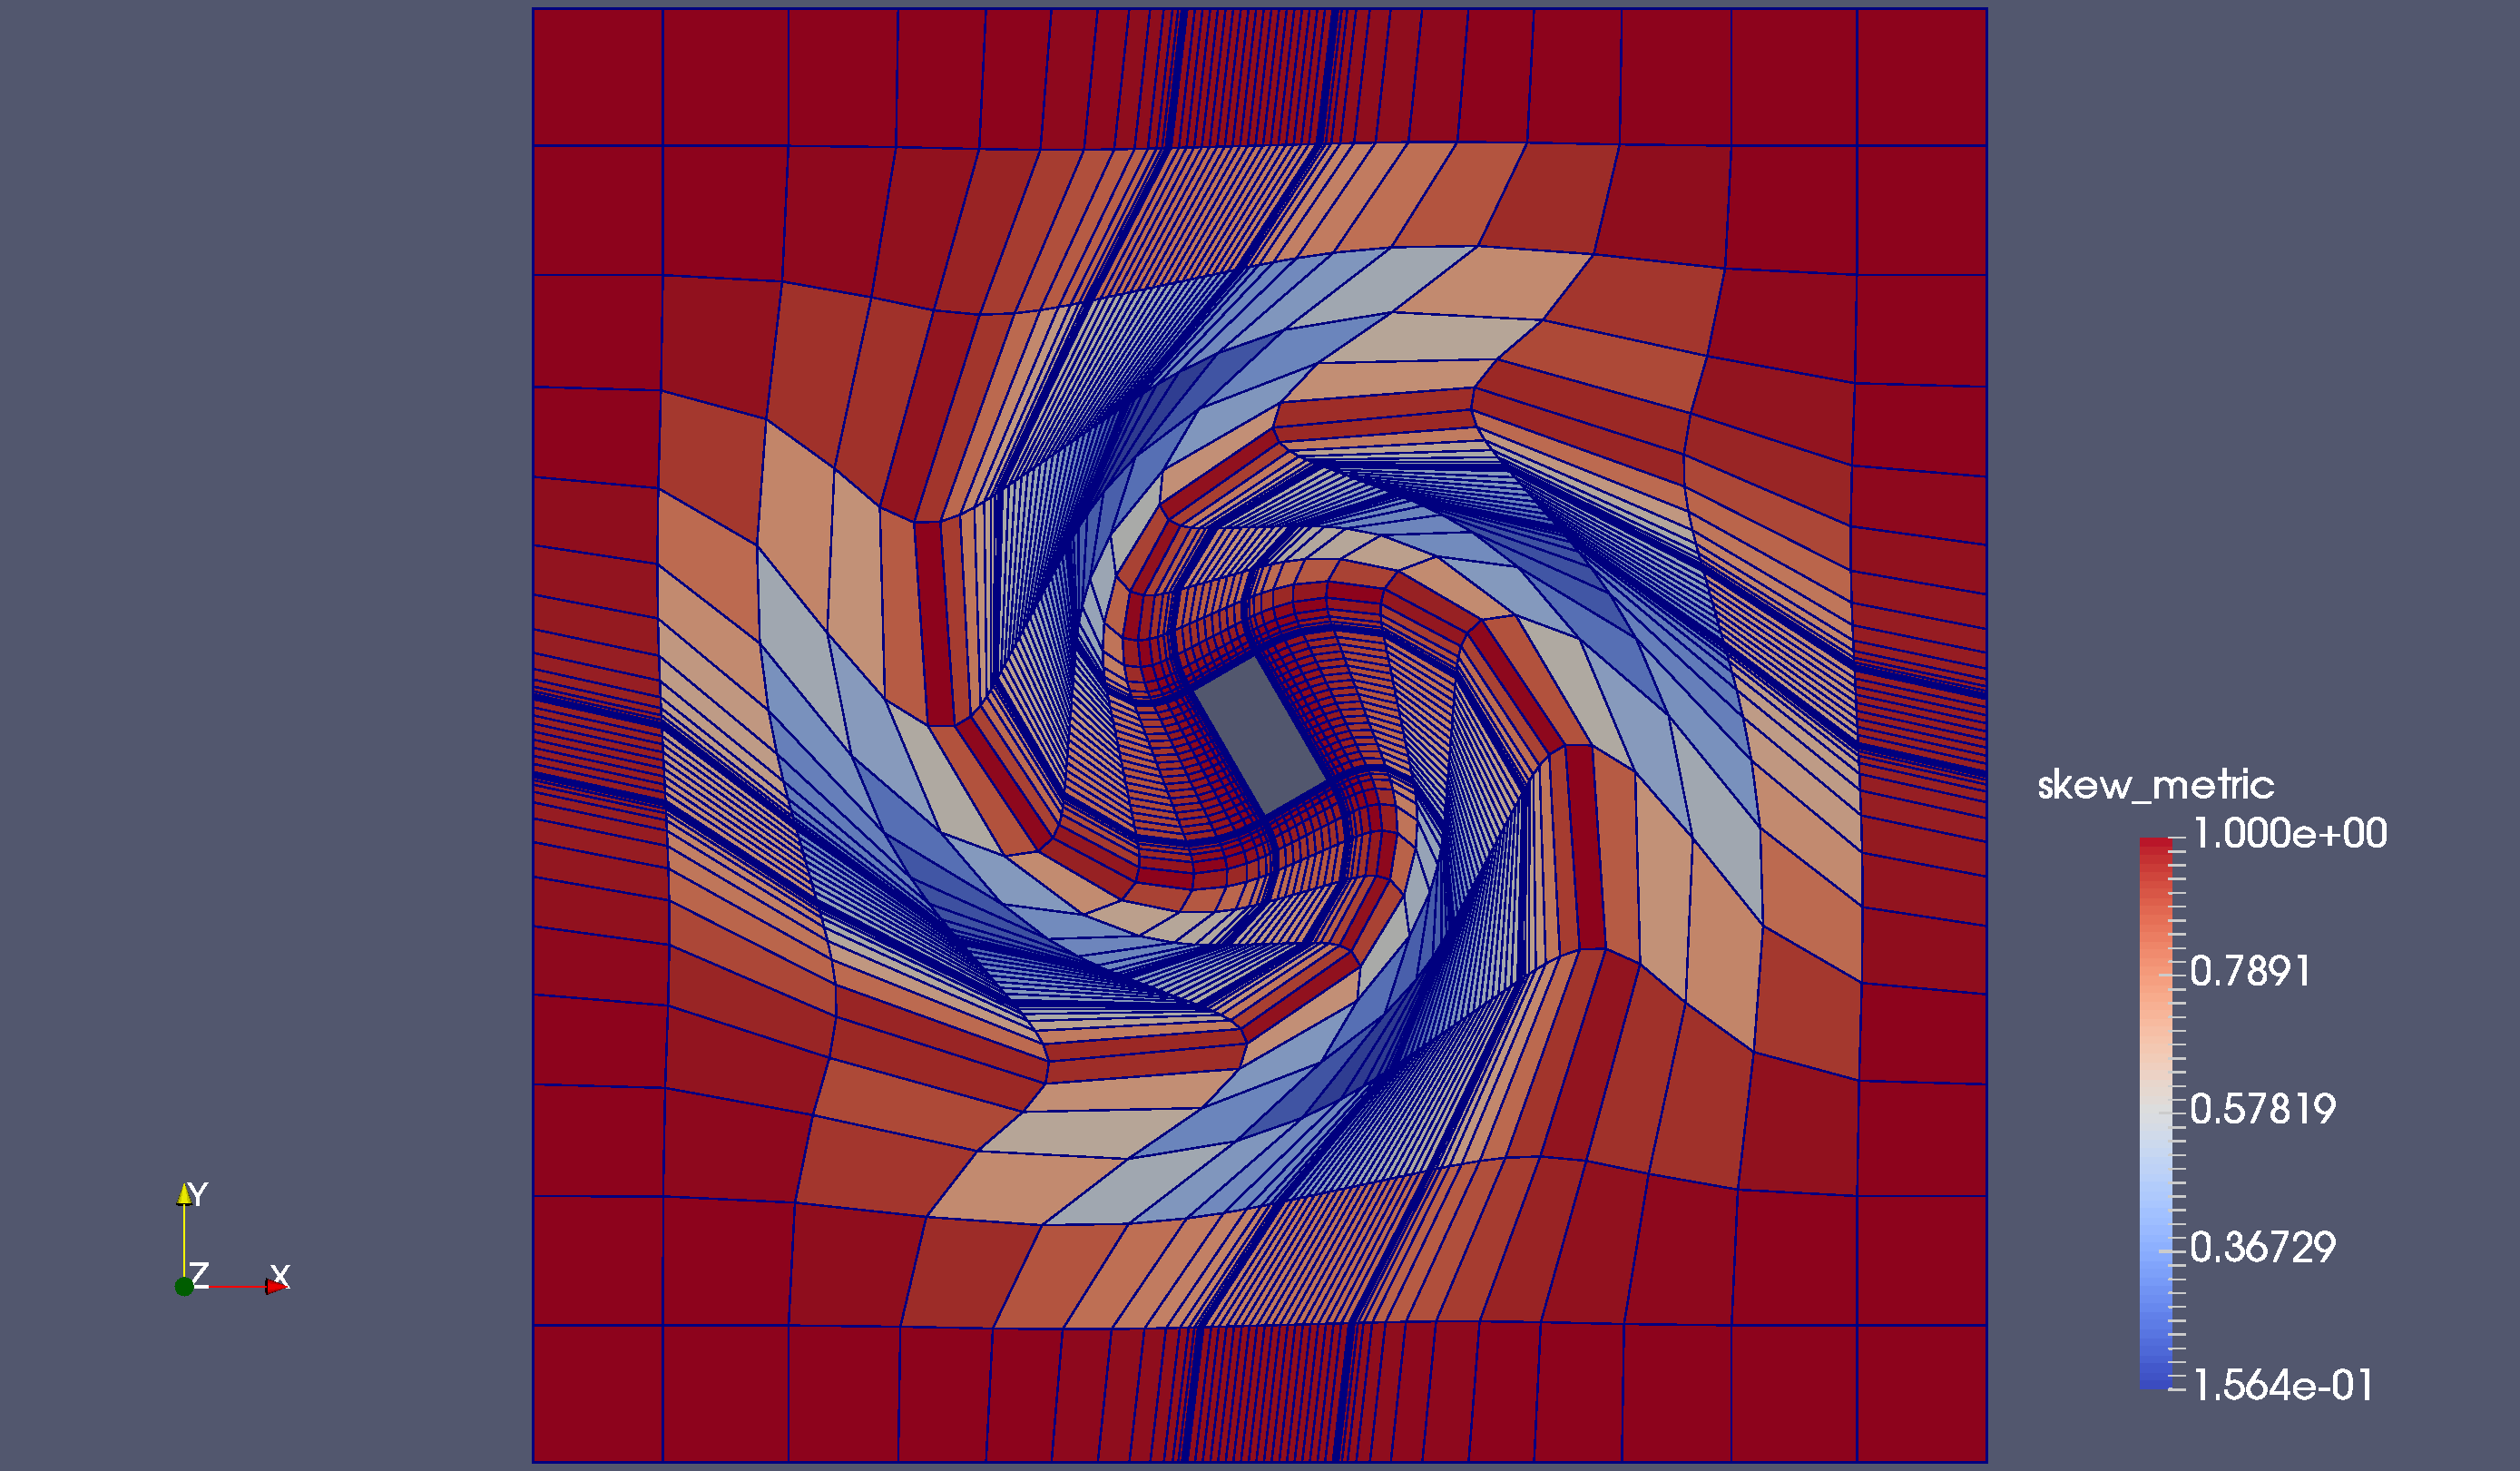
\includegraphics[scale=0.2]{qin-120-quality-withmesh.pdf}
		\caption{Large rotational motion ($120^\circ$) carried out by DGRBF2}
		\label{fig:qin-dgrbf2-120}
	\end{figure}
	RBF can achieve about 117$^\circ$ rotation before giving invalid elements.
	DGRBF2 is very robust for the case it is designed for - large rotational displacements.
\end{frame}

\section{Curved mesh generation}

\begin{frame}{Curved Mesh Generation}
Involves four steps:
\begin{itemize}
	\item Add `high-order' nodes to edges, faces and inside cells
	\item Obtain information about the true boundary, either using CAD data or reconstruction
	\item Determine displacements of boundary nodes and move them
	\item Regularize the interior mesh
\end{itemize}
\begin{figure}
	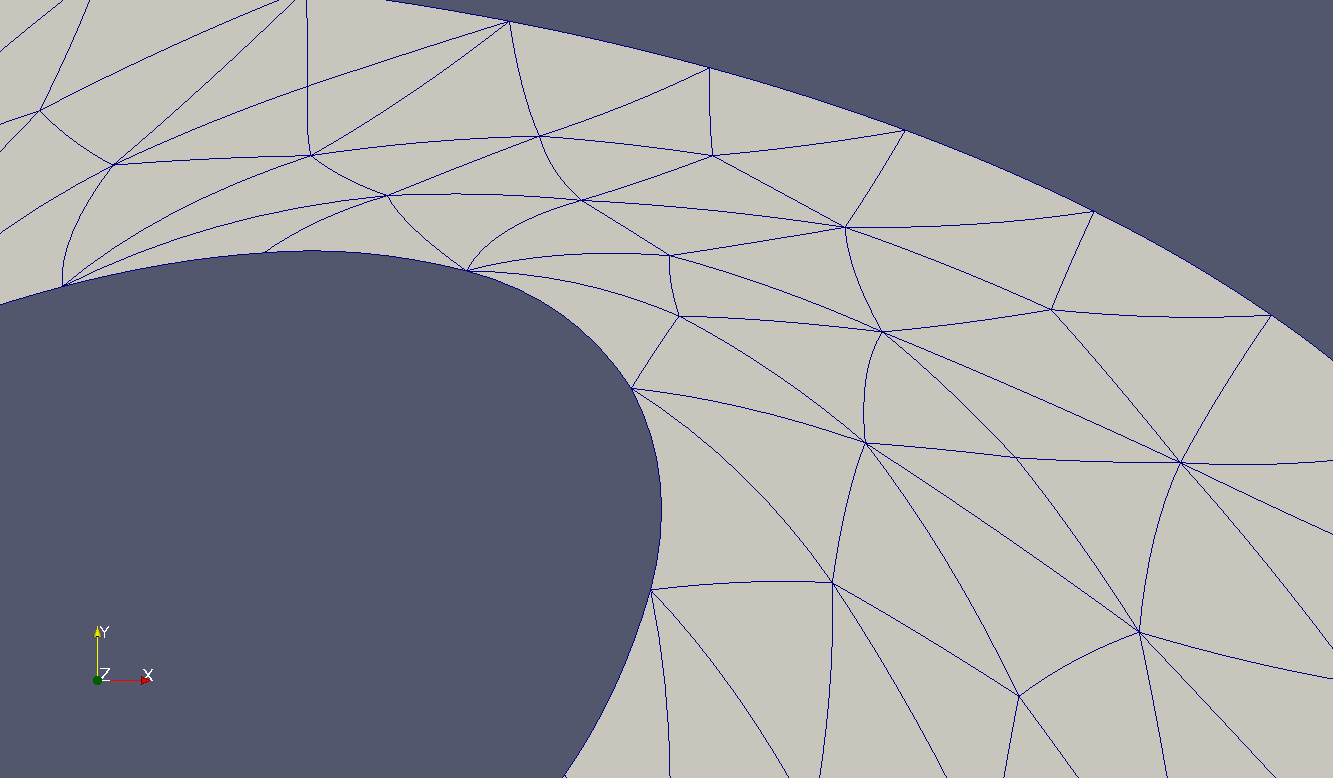
\includegraphics[scale=0.1]{coarse-curved-mesh-zoomed1}
\end{figure}
\end{frame}

\begin{frame}{Boundary reconstruction}
Based on the assumption of smoothness of the boundary, we can reconstruct a piecewise polynomial boundary from a piecewise linear boundary.
\vspace{0.5in}

2D boundary reconstruction code: Reconstructs an almost globally $C^2$ curve using cubic splines.

Corners are detected by comparing normals of consecutive boundary facets.
\end{frame}

\begin{frame}{Interior mesh movement}
Why?
\begin{itemize}
	\item Once boundary nodes are moved, the quality of elements near the boundary deteriorates even for inviscid flow cases. This could worsen the conditioning of the problem.
	\item In case of meshes for turbulent flows, high-aspect-ratio elements in the boundary layer will get invalidated upon boundary movement. This will cause the solver to fail.
\end{itemize}
\end{frame}

\begin{frame}{Interior mesh movement}
Three main ways to achieve a valid and high-quality mesh:
\begin{itemize}
\item Elasticity-based methods (Peraire and Persson \cite{curve:persson}, Hartmann \cite{curve:hartmann}, many others)
\item Interpolation methods (Z.J. Wang \cite{curve:meshcurve} and others)
\item Optimization (Toulorge \emph{et. al.} \cite{gmsh:untangling})
\end{itemize}
\end{frame}

\begin{frame}{Curved mesh quality}
We need a way for measuring curved mesh quality independent of linear mesh quality. This is done as a post-processing step using the plugin `AnalyseCurvedMesh' available in Gmsh \footfullcite{gmsh:quality}. The quantity computed by this plugin is given as
\begin{equation} 
m_i = \frac{\inf_{\mathbf{x}\in\Omega_i}\det \mathbf{J}_i(\mathbf{x})}{\det \mathbf{J_l}_i},
\end{equation}
It measures the `distortion' of the element from the corresponding linear element.
\end{frame}

\subsection{Viscous 3-component airfoil}
\begin{frame}{Viscous 3-component airfoil}
We reconstruct a high-order boundary using cubic splines. Interior mesh movement is compared using linear elasticity, RBF and stiffened linear elasticity (SLE).
\begin{figure}
	\centering
	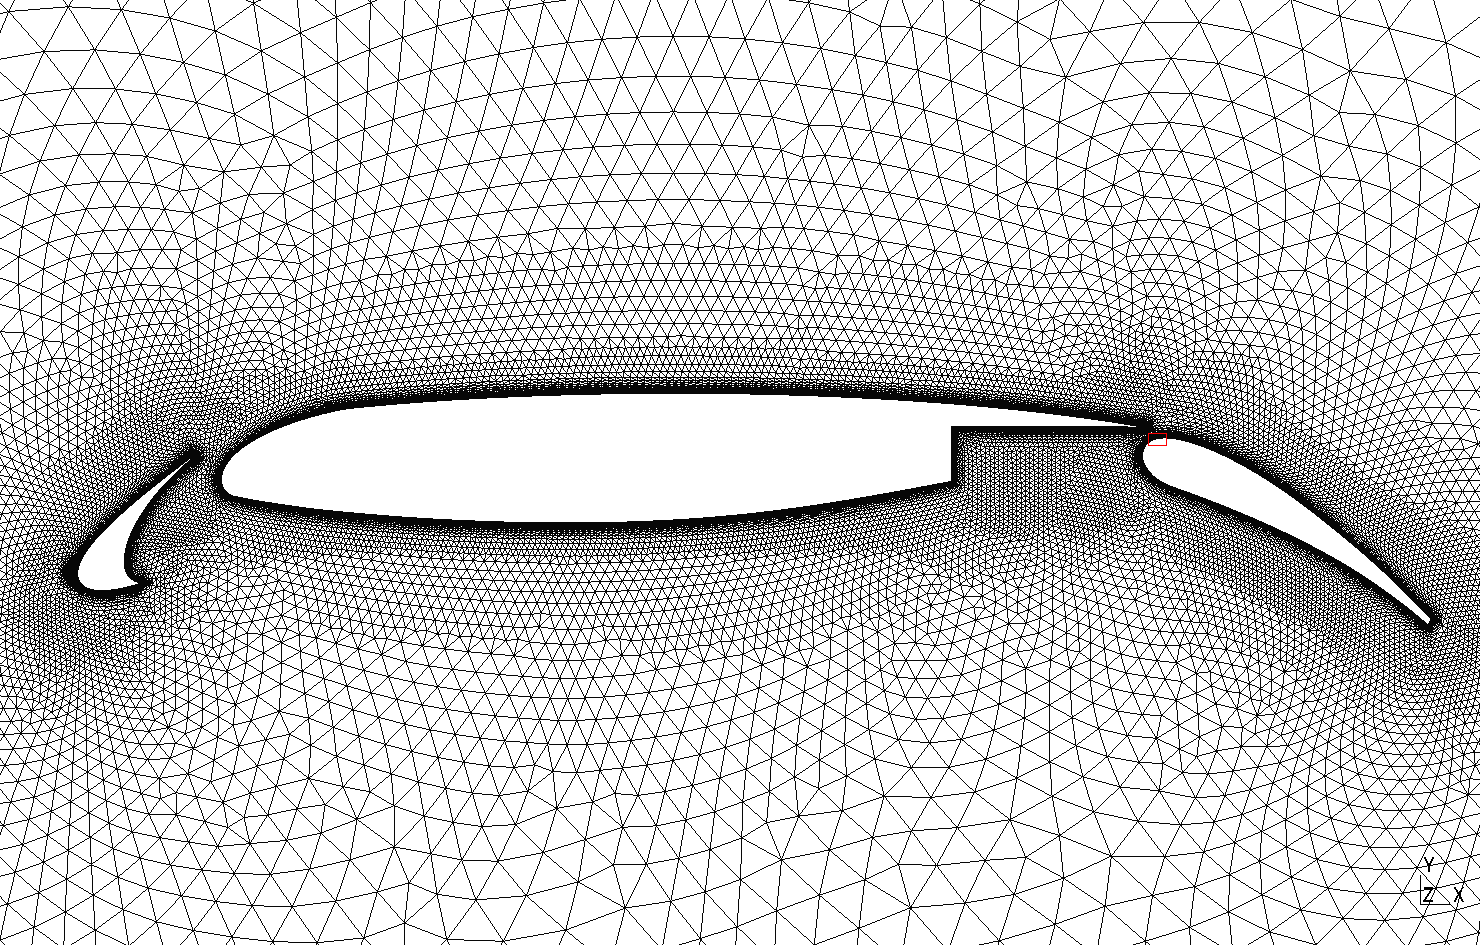
\includegraphics[width=150.0pt]{3compblack}
	\caption{Boundary-layer mesh of multi-element airfoil}
\end{figure}
\end{frame}

\begin{frame}
	 \begin{figure}
	 	\centering
	 	\subfloat{
	 		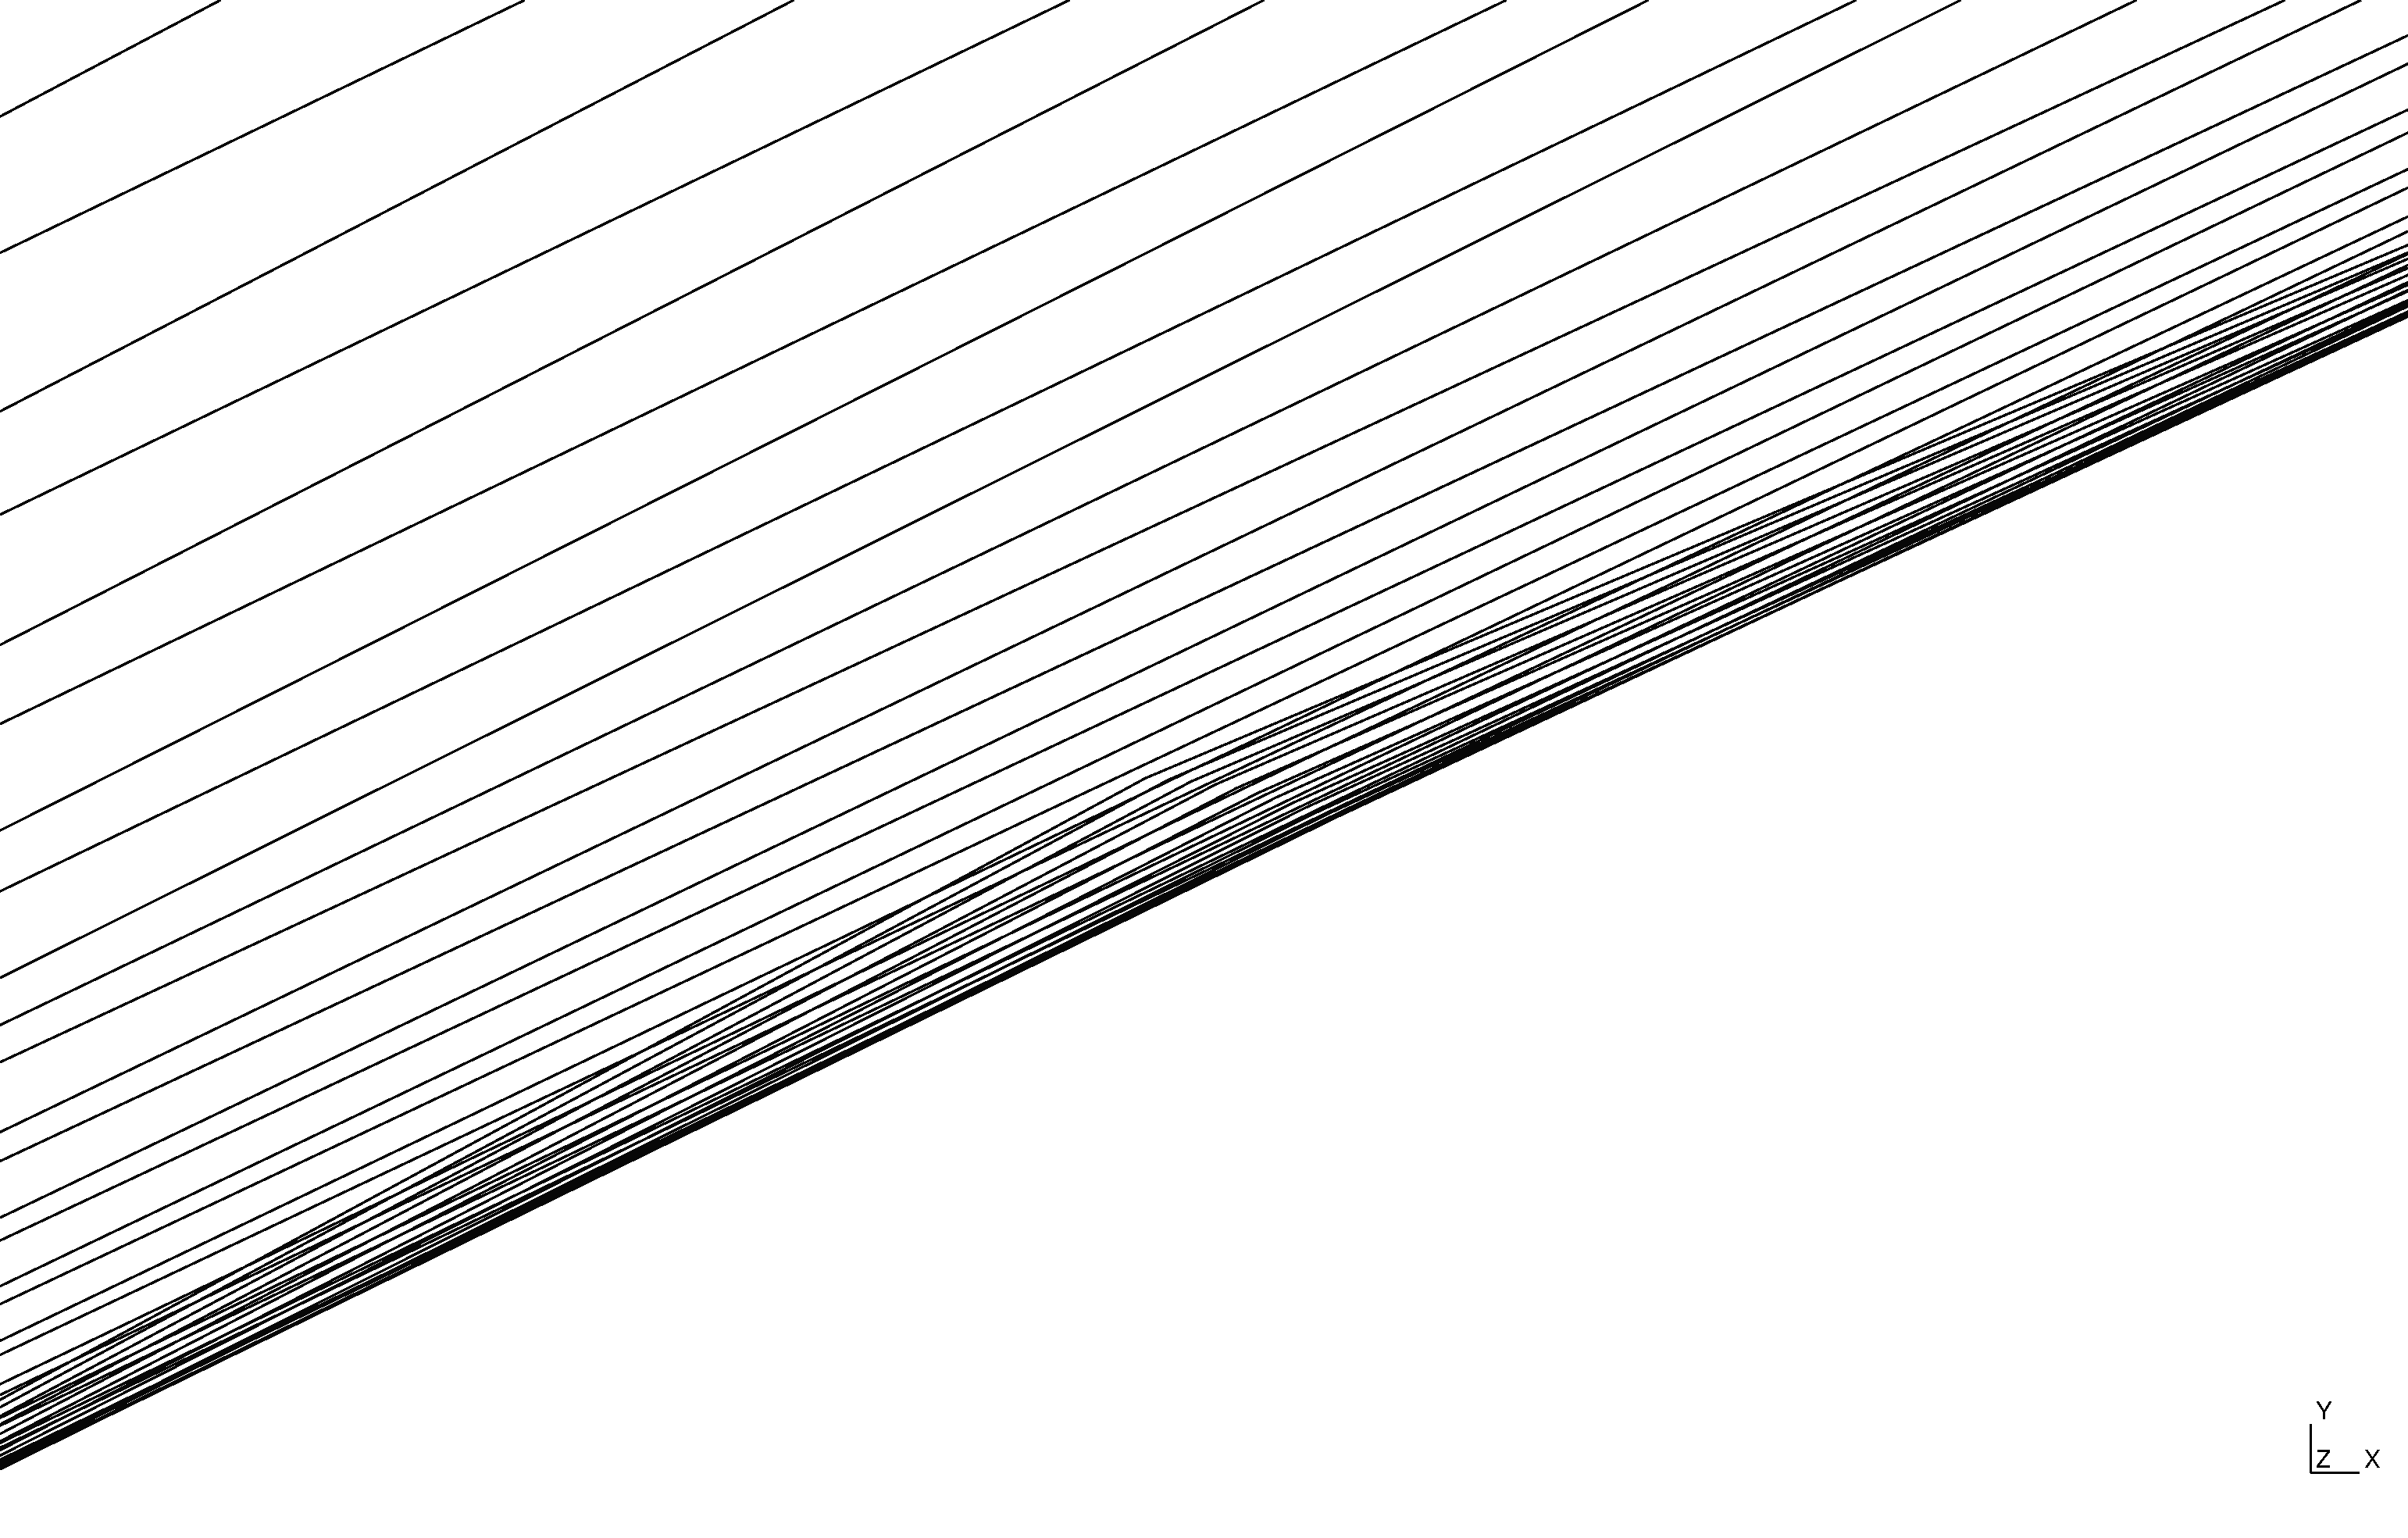
\includegraphics[width=150.0pt]{3comp-elast-vzoomedblk.pdf}
	 	}
	 	\subfloat{
	 		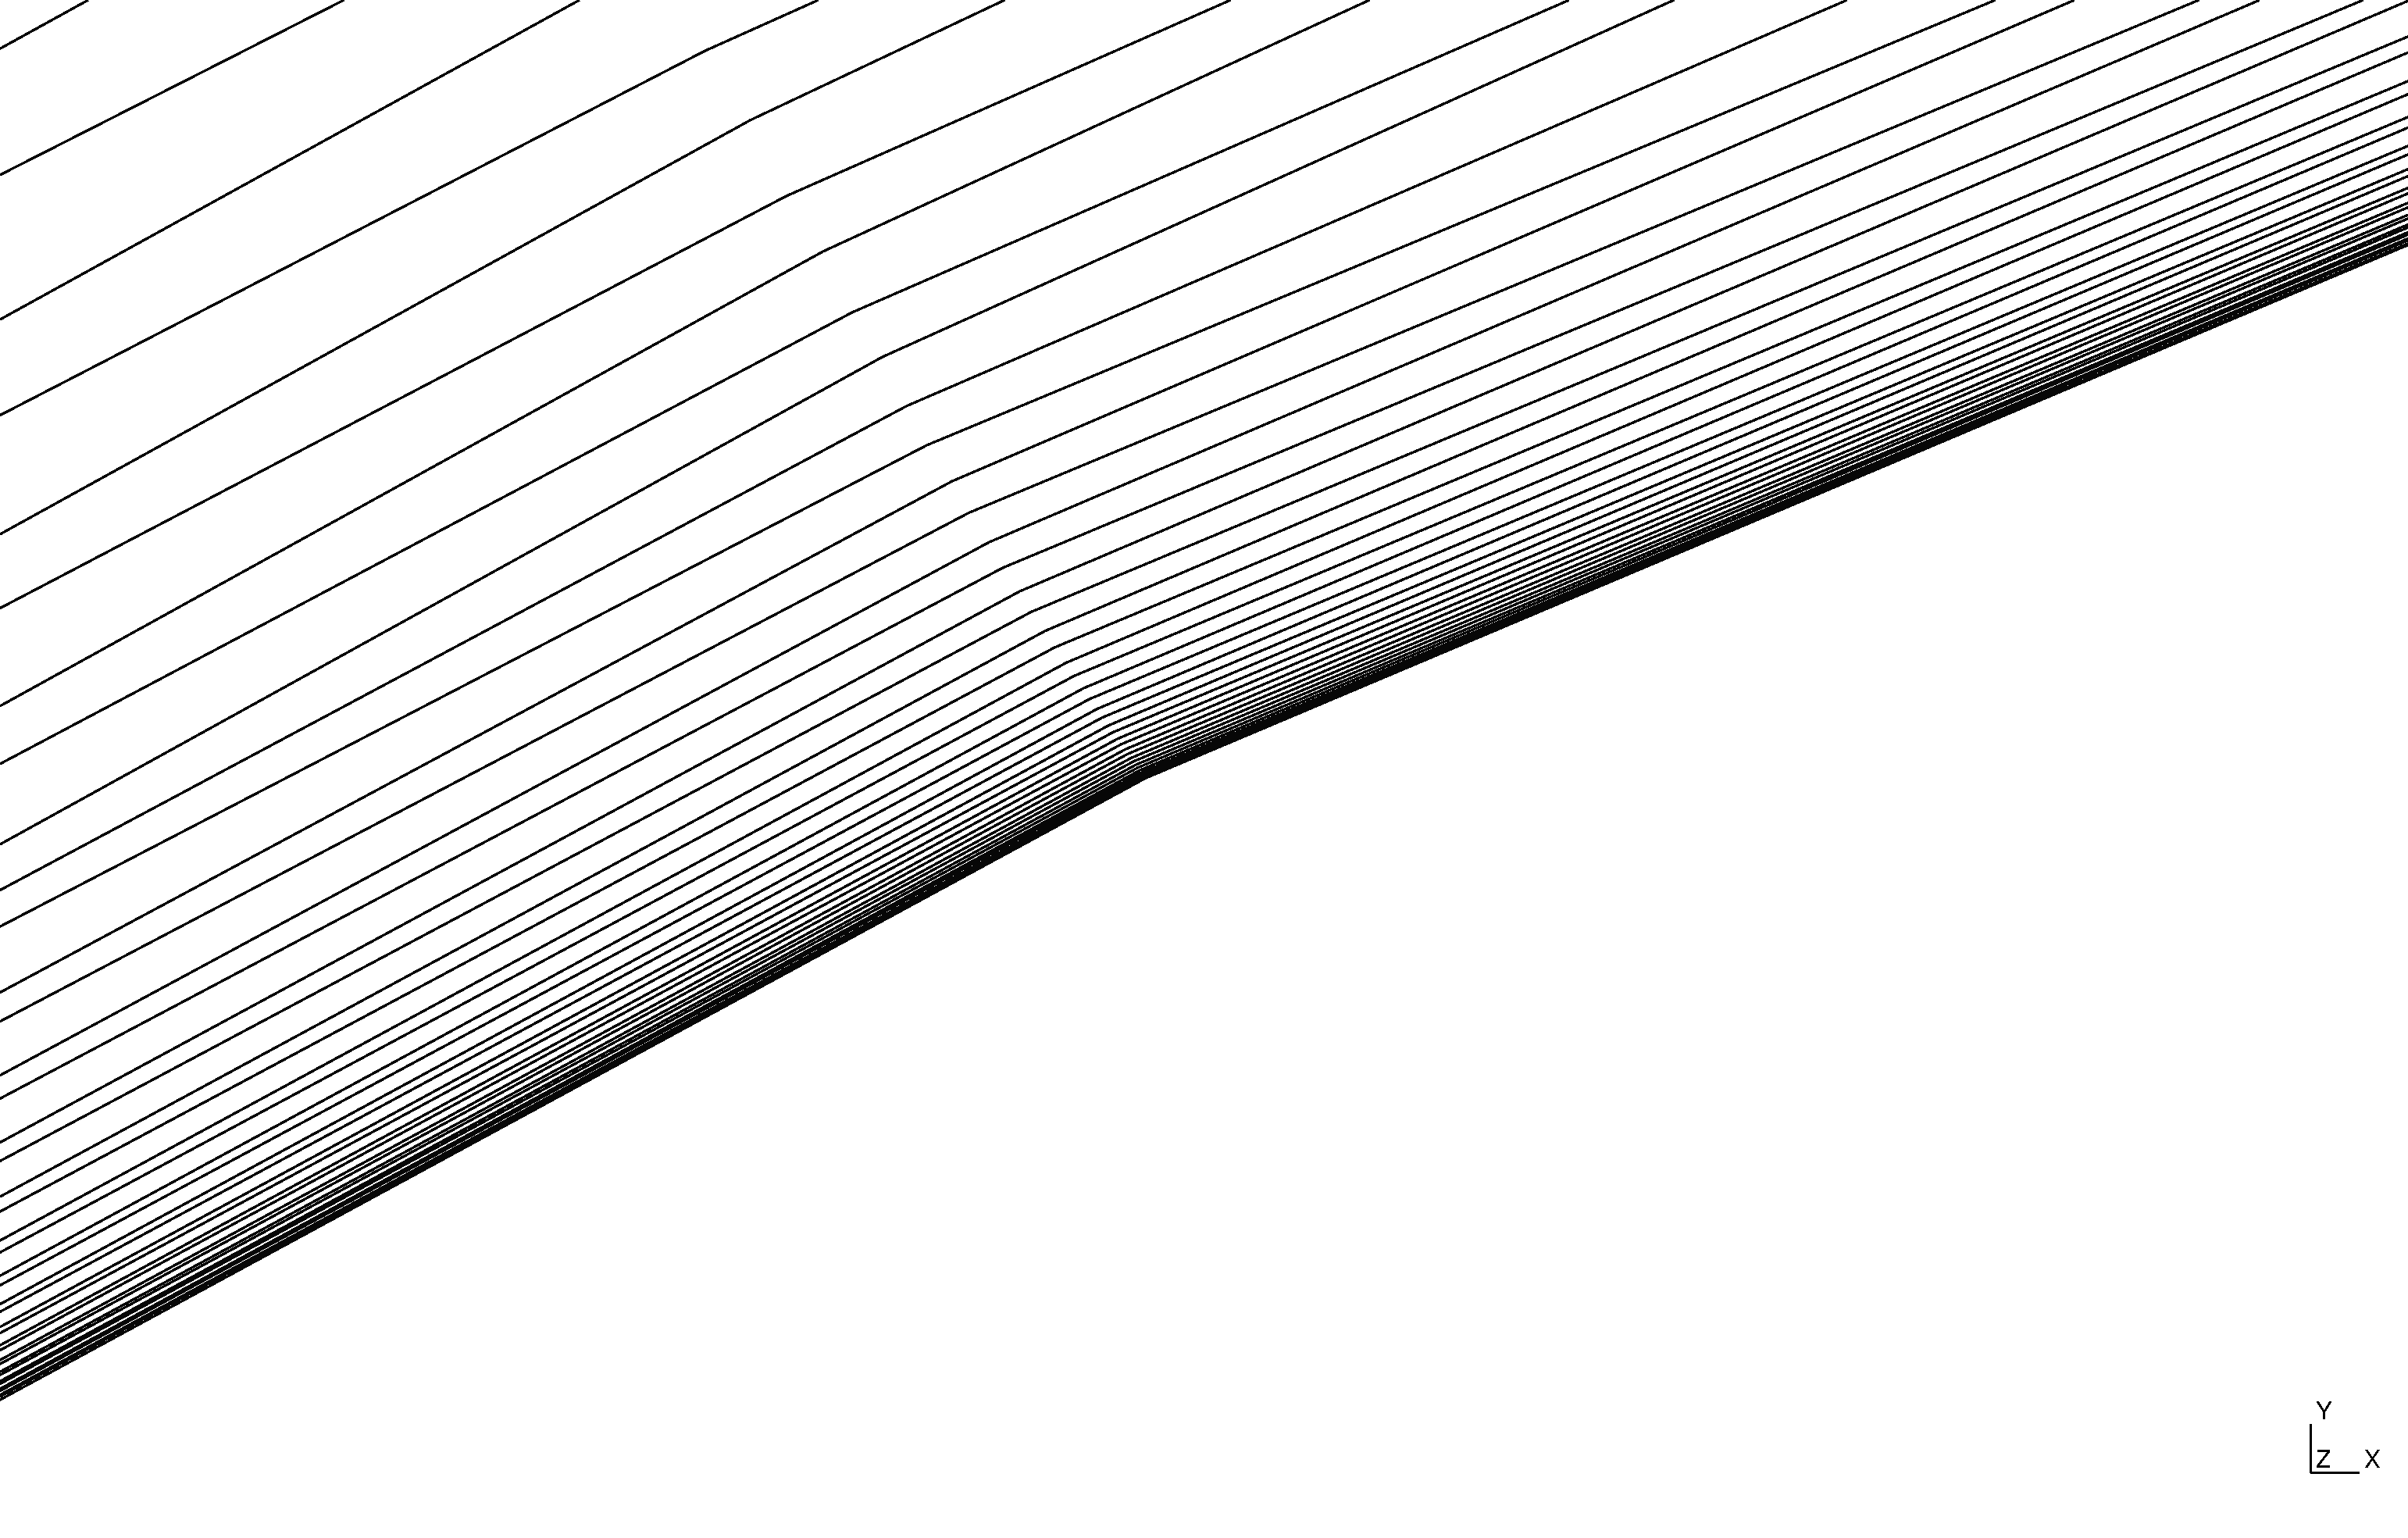
\includegraphics[width=150.0pt]{3comp-rbf-vzoomedblk.pdf}
	 	}
	 	\caption{Portion of quadratic viscous mesh for multi-element airfoil, showing a boundary face in the flap, generated by linear elasticity (left) and RBF (right) methods}
	 	\label{fig:tangled2}
	 \end{figure}
	 Regular linear elasticity does not work.
\end{frame}

\begin{frame}
	\begin{figure}
		\centering
		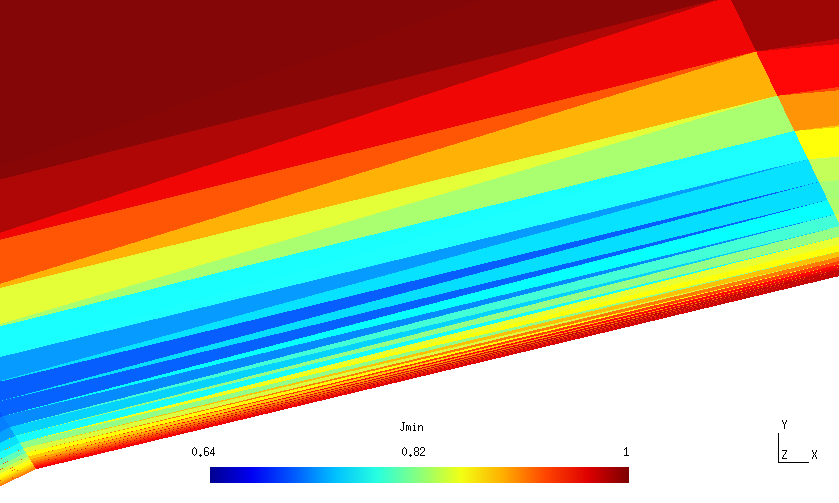
\includegraphics[scale=0.3]{3comp-rbf-zoomed-jacobians2.png}
		\caption{Minimum scaled Jacobian over each element for a portion mesh generated by RBF interpolation}
		\label{fig:rbf-jacobians}
	\end{figure}
\end{frame}
\begin{frame}
\begin{figure}
	\centering
	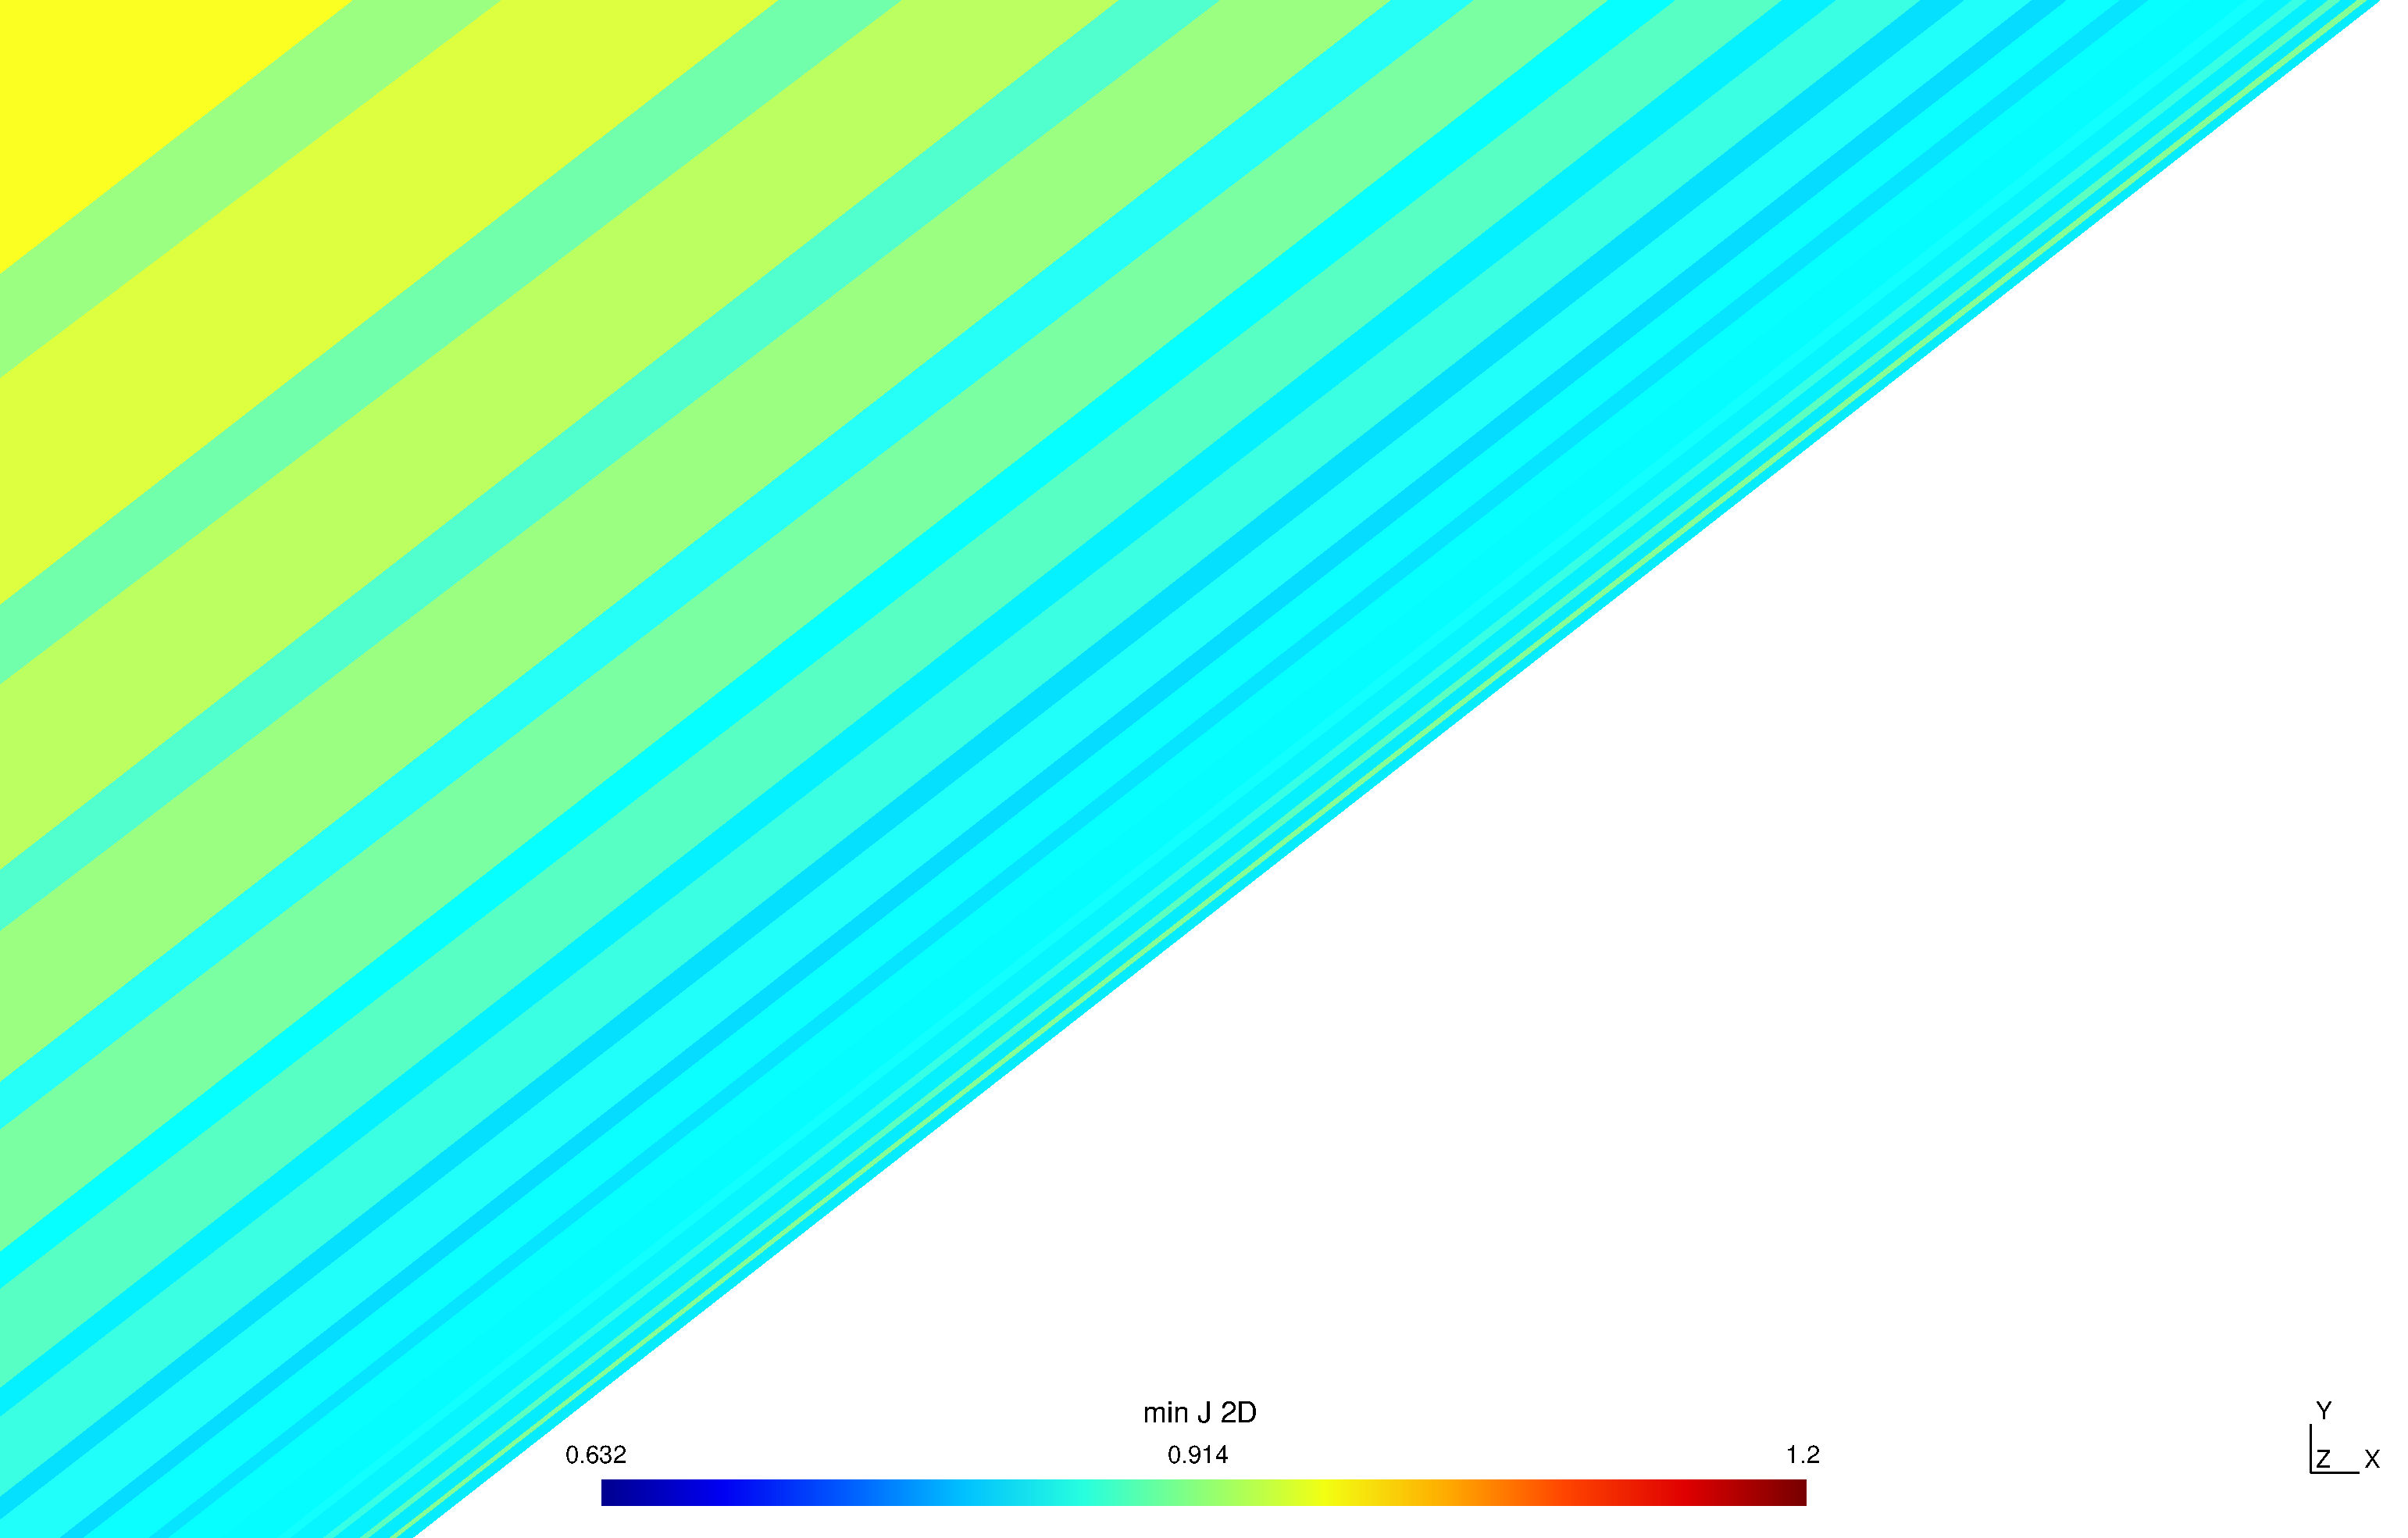
\includegraphics[scale=0.2]{3comp_curved_elaststiff_vzoomed_jac}
	\caption{A portion curved mesh generated by stiffened elasticity method; minimum scaled Jacobian over each element is shown}
	\label{fig:3compstiffelastjac}
\end{figure}
\end{frame}
\begin{frame}
\begin{figure}
	\centering
	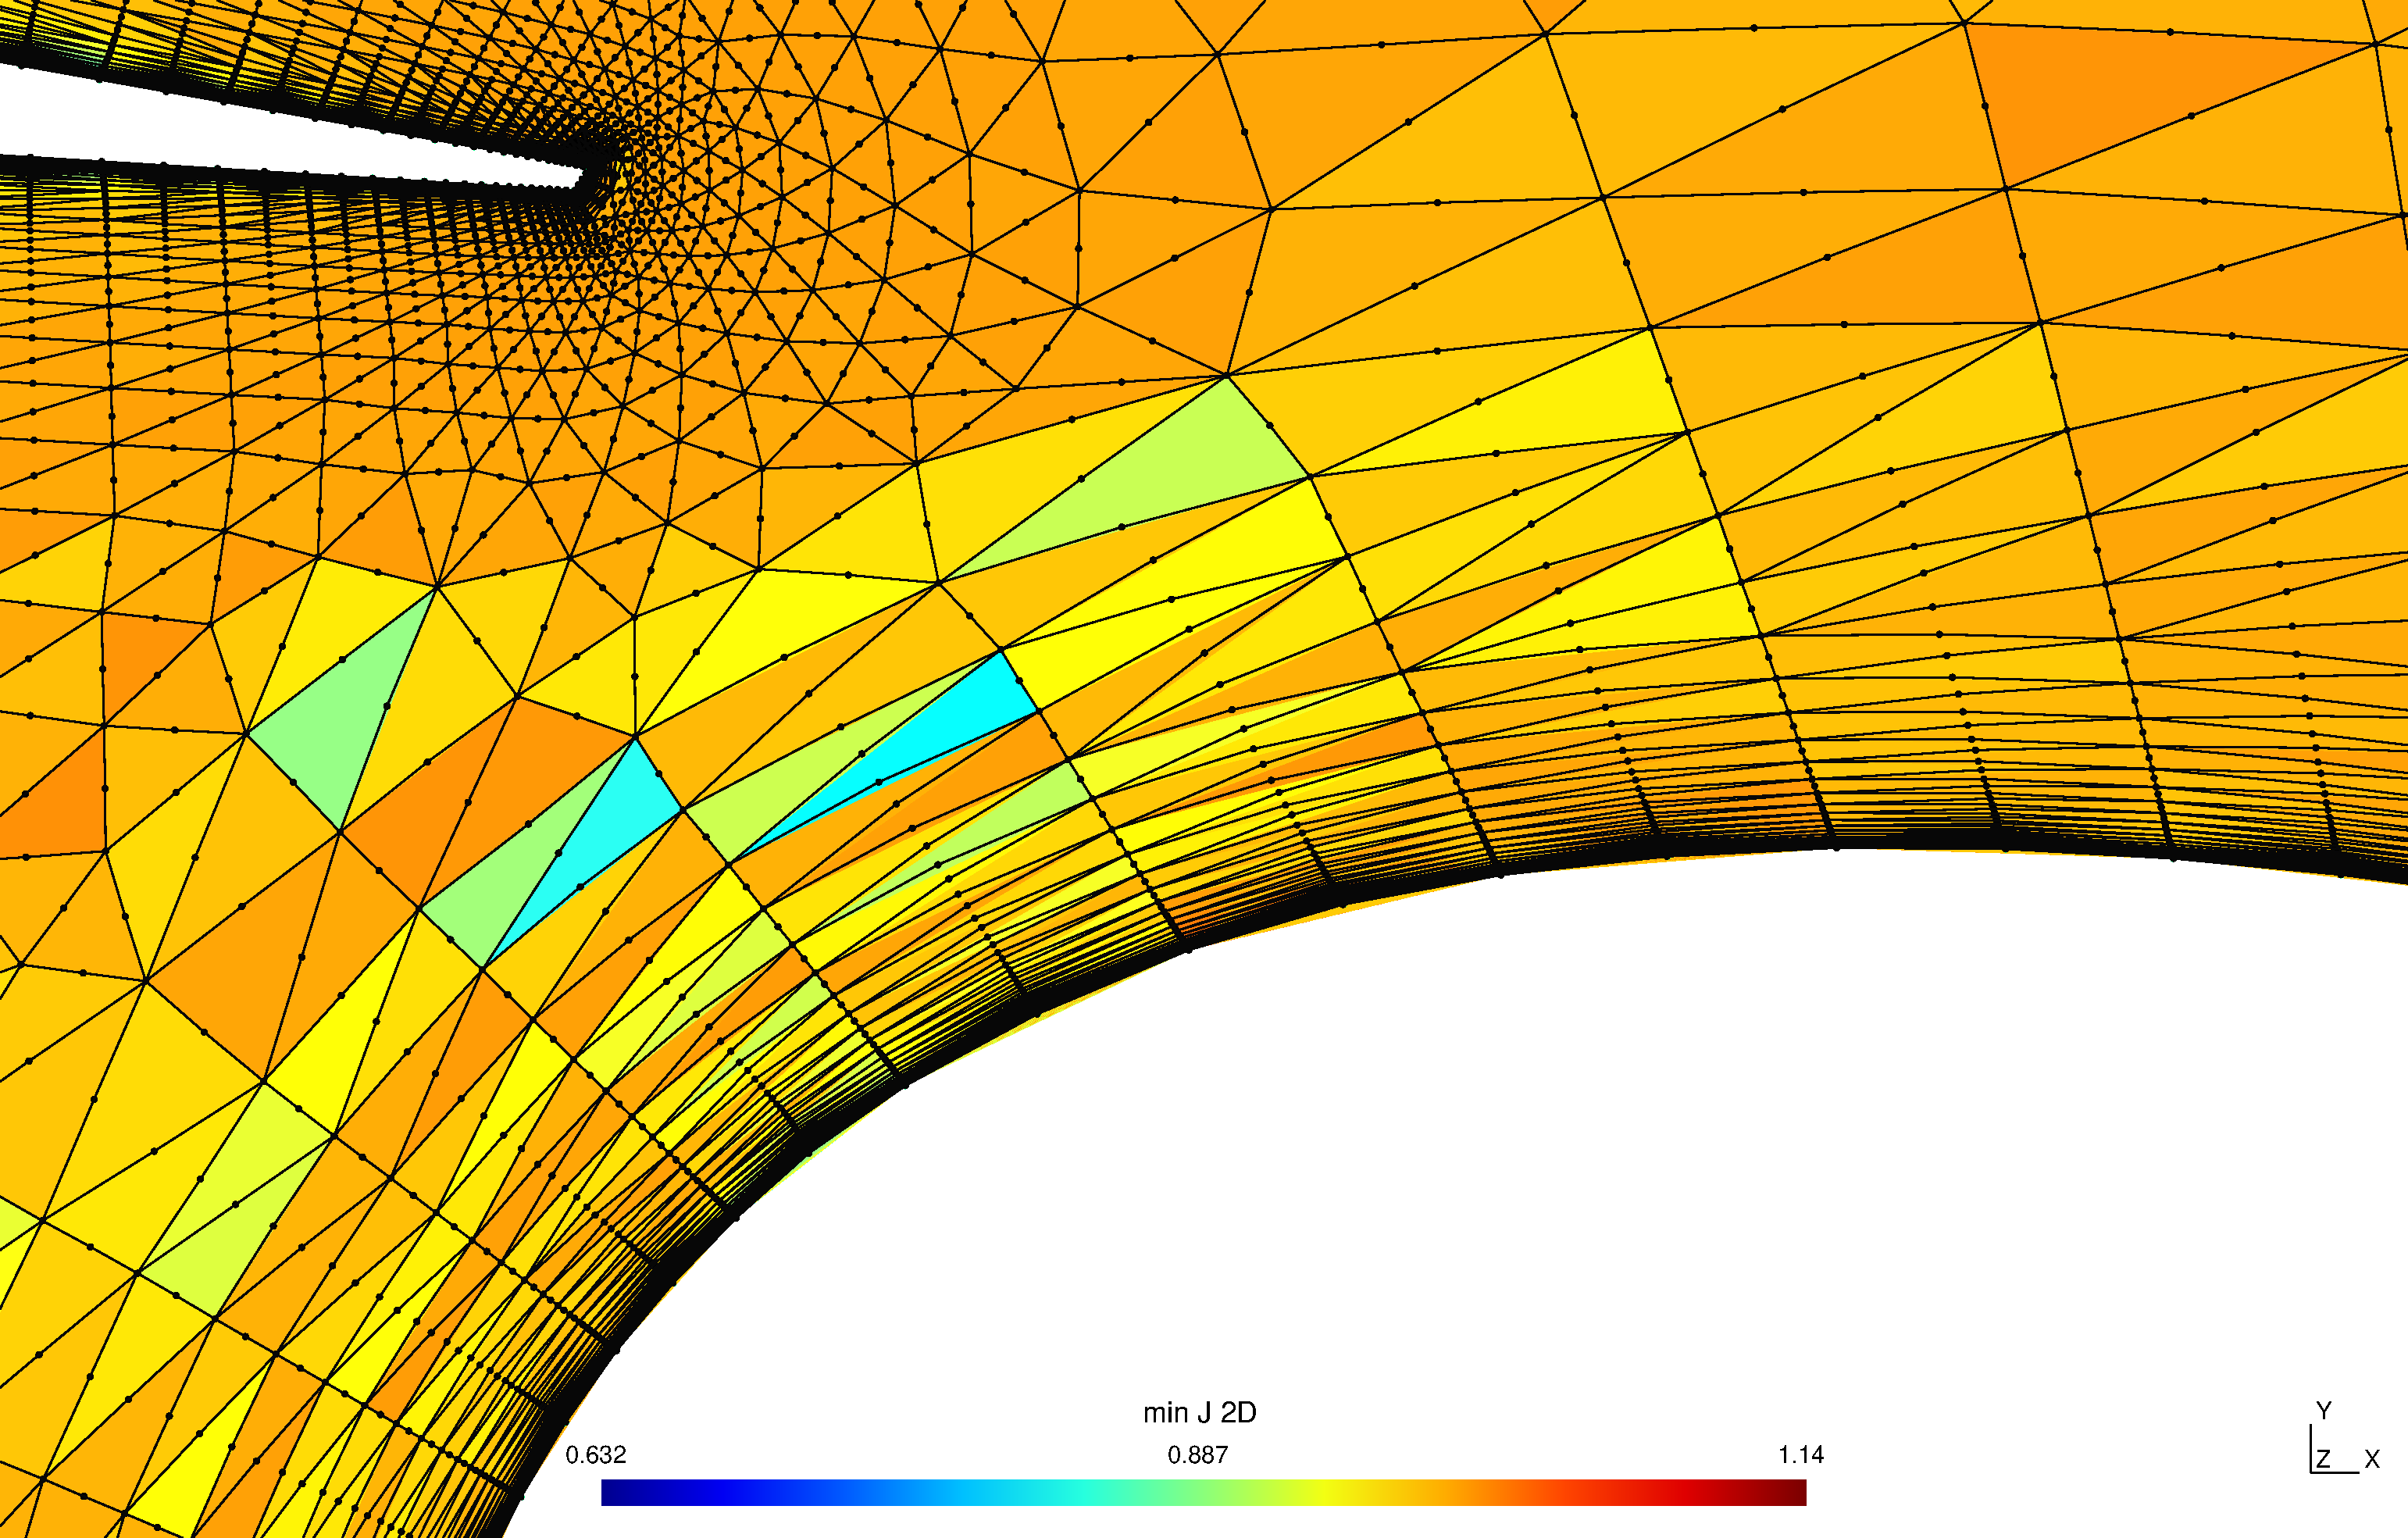
\includegraphics[scale=0.2]{3comp-stiffelast-zoomed}
	\caption{An illustrative example of a curved mesh generated by stiffened elasticity method; minimum scaled Jacobian over each element is shown}
	\label{fig:3compstiffelast}
\end{figure}
\end{frame}

\begin{frame}{Performance}
	\fontsize{8pt}{10}\selectfont
	Solutions are computed by a point-Jacobi-preconditioned conjugate gradient solver.
	\begin{table}
		\begin{tabular}{|c|c|c|c|c|c|}
			\hline
			Method & Parameters & Min. quality & Avg. quality & Time & Solver iterations \\
			\hline
			\multirow{2}{0.5in}{SLE} & $\chi=2.75$ & 0.632 & 0.994922 & 19.3s & 324 \\
			& $\chi=2.9$ & 0.632 & 0.994535 & 24.4s & 423 \\
			\hline
			\multirow{4}{0.5in}{RBF} & 1-step $r_s=0.04$ & 0.640 & 0.991093 & 1.86s & 365 x 2 \\
			&   1-step $r_s=0.08$ & 0.639 & 0.991562 & 1.88s & 1150 x 2\\
			&   1-step $r_s=0.12$ & 0.637 & 0.99159  & 1.89s & 2295 x 2 \\
			&   2-step $r_s=0.04$ & 0.641 & 0.991099 & 2.58s & 365 x 4\\
			\hline
		\end{tabular}
		\caption{Comparison of RBF (radial basis function) and SLE (stiffened linear elasticity) methods}
		\label{tab:rbfelast}
	\end{table}
\end{frame}

\subsection{3D Bump Channel Turbulent Flow Case}
\begin{frame}{3D Bump Channel Turbulent Flow Case}
Reynolds-averaged Navier-Stokes (RANS) flow simulation test case from the NASA Turbulence models website \cite{case:bump3d}.

The mesh is a hexahedral structured grid.

Boundary displacements were first obtained from the analytical expression for the bump given on the website. The solver used for RBF is a sparse LU decomposition.
\begin{figure}
	\centering
	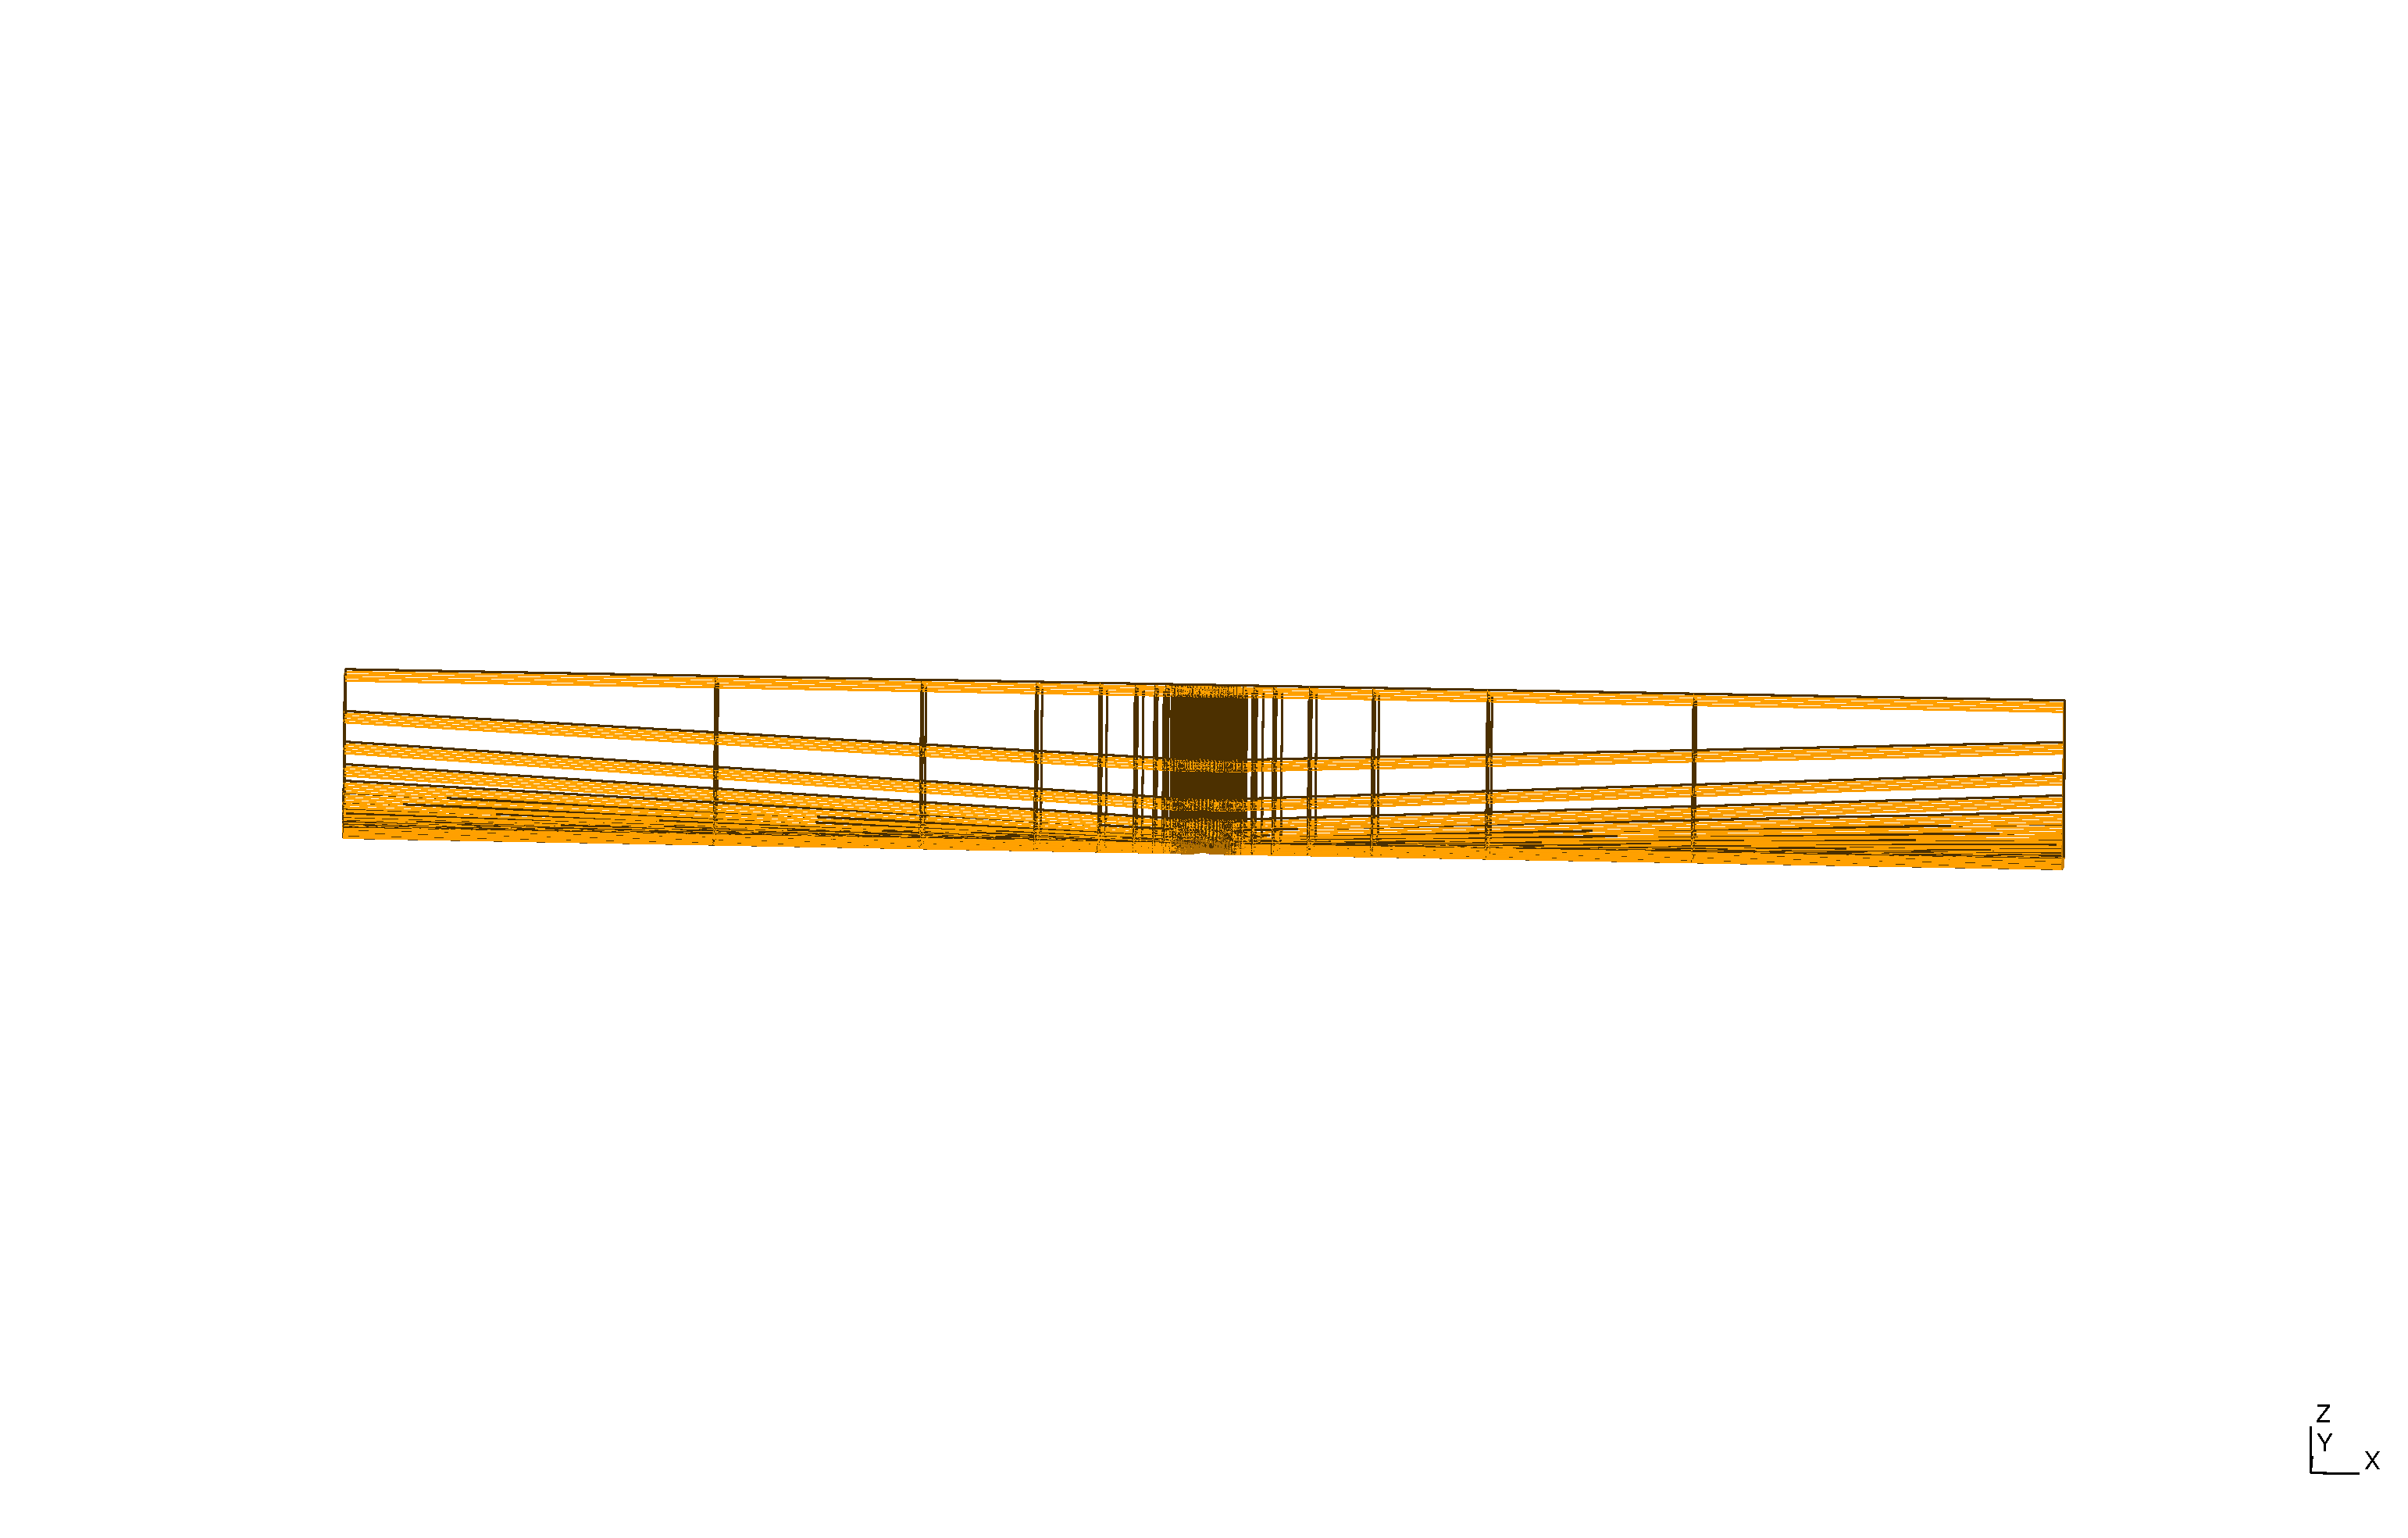
\includegraphics[scale=0.2]{bump3d-vcoarse2}
	\caption{Coarsest curved mesh of 3D bump channel}
	\label{fig:bump3d}
\end{figure}
\end{frame}

\begin{frame}
	\begin{figure}
		\centering
		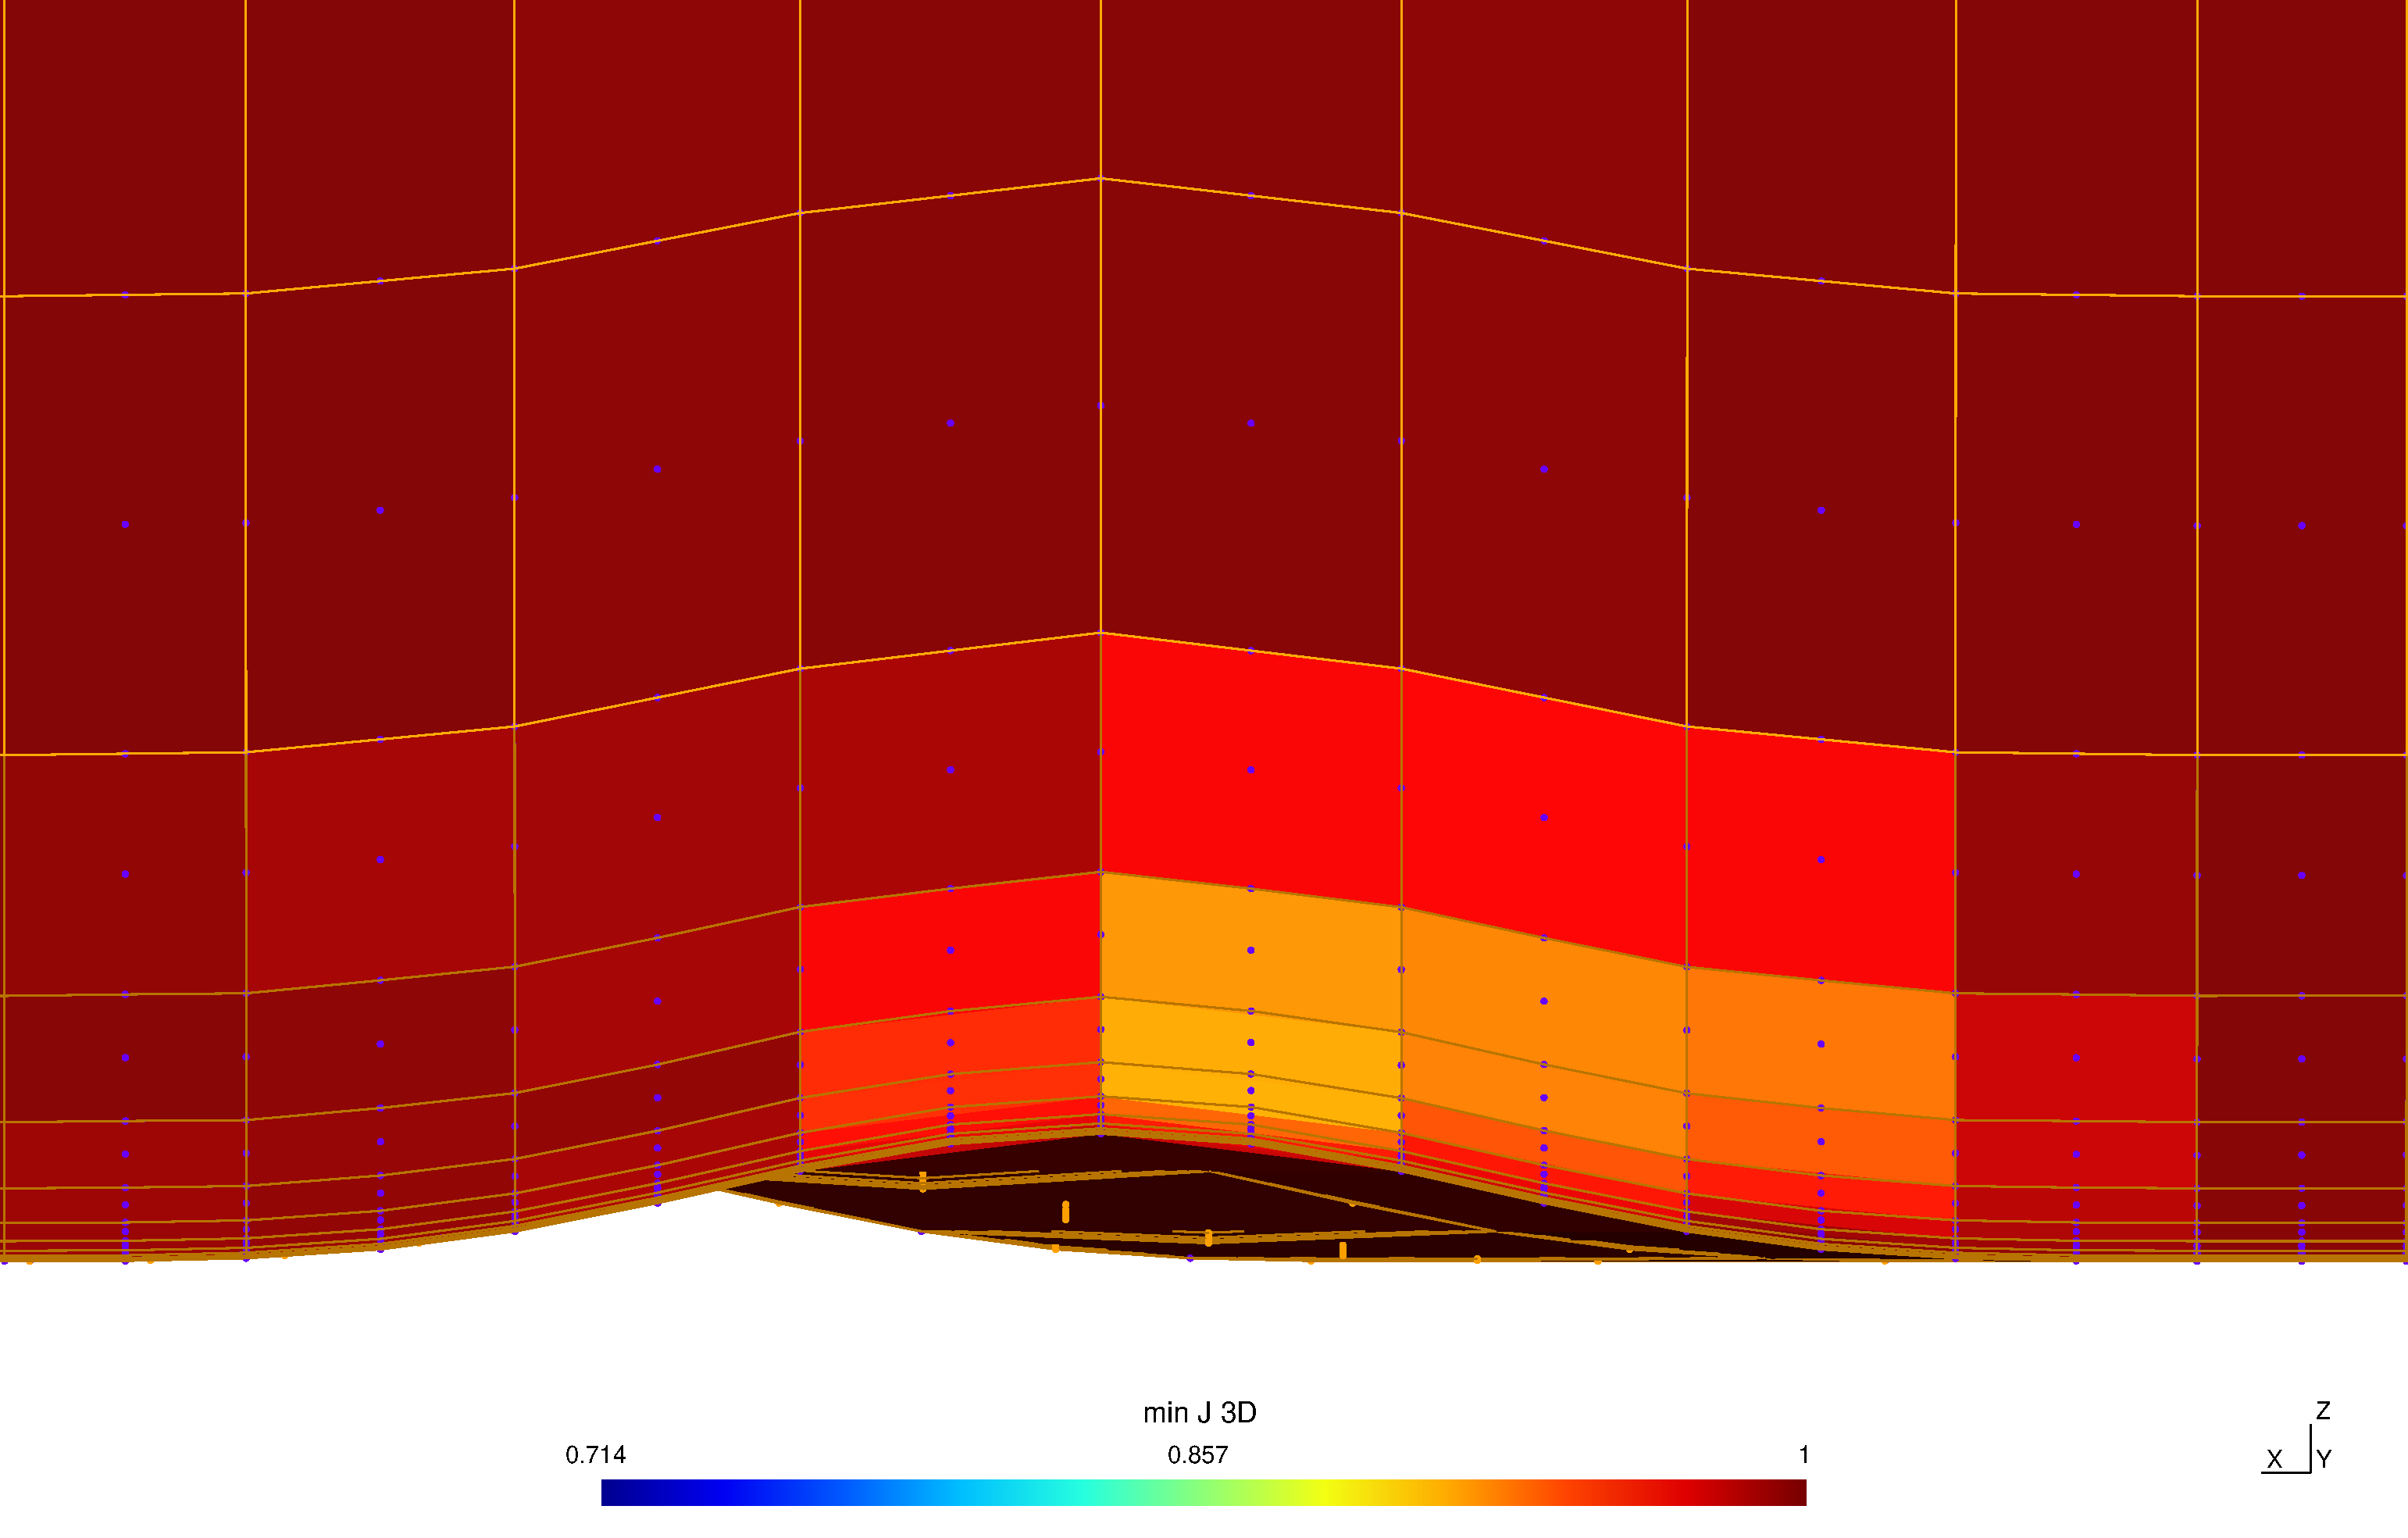
\includegraphics[scale=0.2]{bump3d-vcoarse-quality}
		\caption{Minimum scaled Jacobian of coarse curved mesh of 3D bump channel}
		\label{fig:bump3d-coarse-jac}
	\end{figure}
\end{frame}

\begin{frame}{Performance of curved mesh generator}
	\begin{table}
		\centering
		\begin{tabular}{|c|c|c|c|}
			\hline
			& Coarse & Medium & Fine \\
			\hline
			No. of points 				& 32,841 & 243,729	& 1,875,489 \\
			No. of boundary points		& 2,304	& 8,704		& 33,792 \\
			Support radius				& 0.06	& 0.06		& 0.04 \\
			Minimum quality			& 0.714	& 0.852		& 0.926 \\
			Wall-clock time			& 0.68s	& 12.6s		& 338s \\
			\hline
		\end{tabular}
		\caption{Summary of 3D bump channel curved mesh generation}
	\end{table}
\end{frame}

\begin{frame}
Results from RANS simulation run by rDGFLO \footfullcite{solver}
\begin{itemize}
	\item Spalart-Allmaras eddy-viscosity model
	\item DG P1
	\item HLLC and Bassi Rebay 2 numerical fluxes
	\item First order in time, implicit time stepping
	\item LU SGS preconditioned GMRES solver
\end{itemize}
Results obtained for the RBF mesh are compared with those obtained from another curved mesh; the latter obtained by agglomeration of finer meshes.
\end{frame}

\begin{frame}{Residual convergence for mass flux}
\begin{figure}
	\centering
	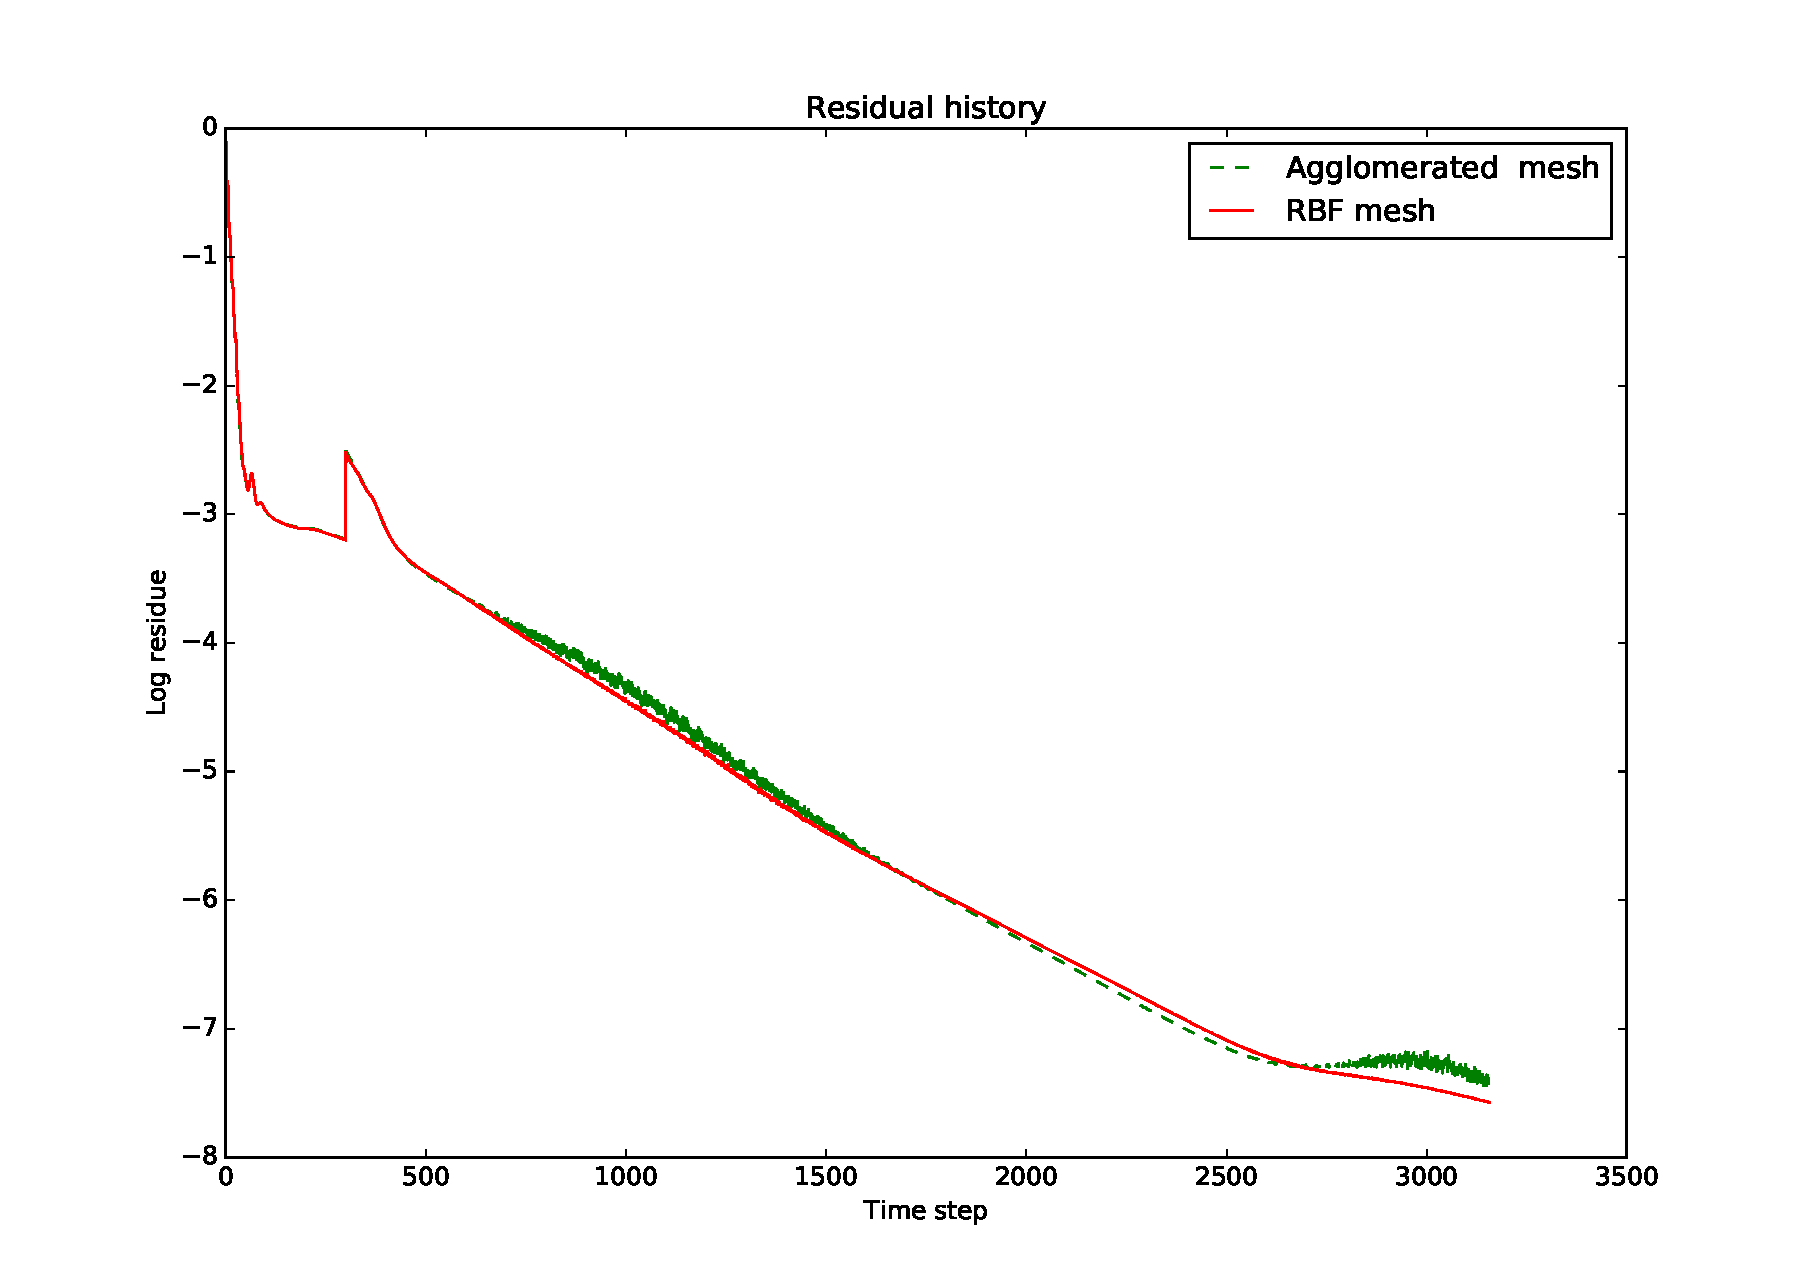
\includegraphics[scale=0.27]{solver-convergence}
	\caption{Comparison of mass-flux residual convergence history with time steps for implicit DG P1 solution}
	\label{fig:resconvergence}
\end{figure}
\end{frame}

\begin{frame}{Grid convergence for $C_d$}
\begin{figure}
	\centering
	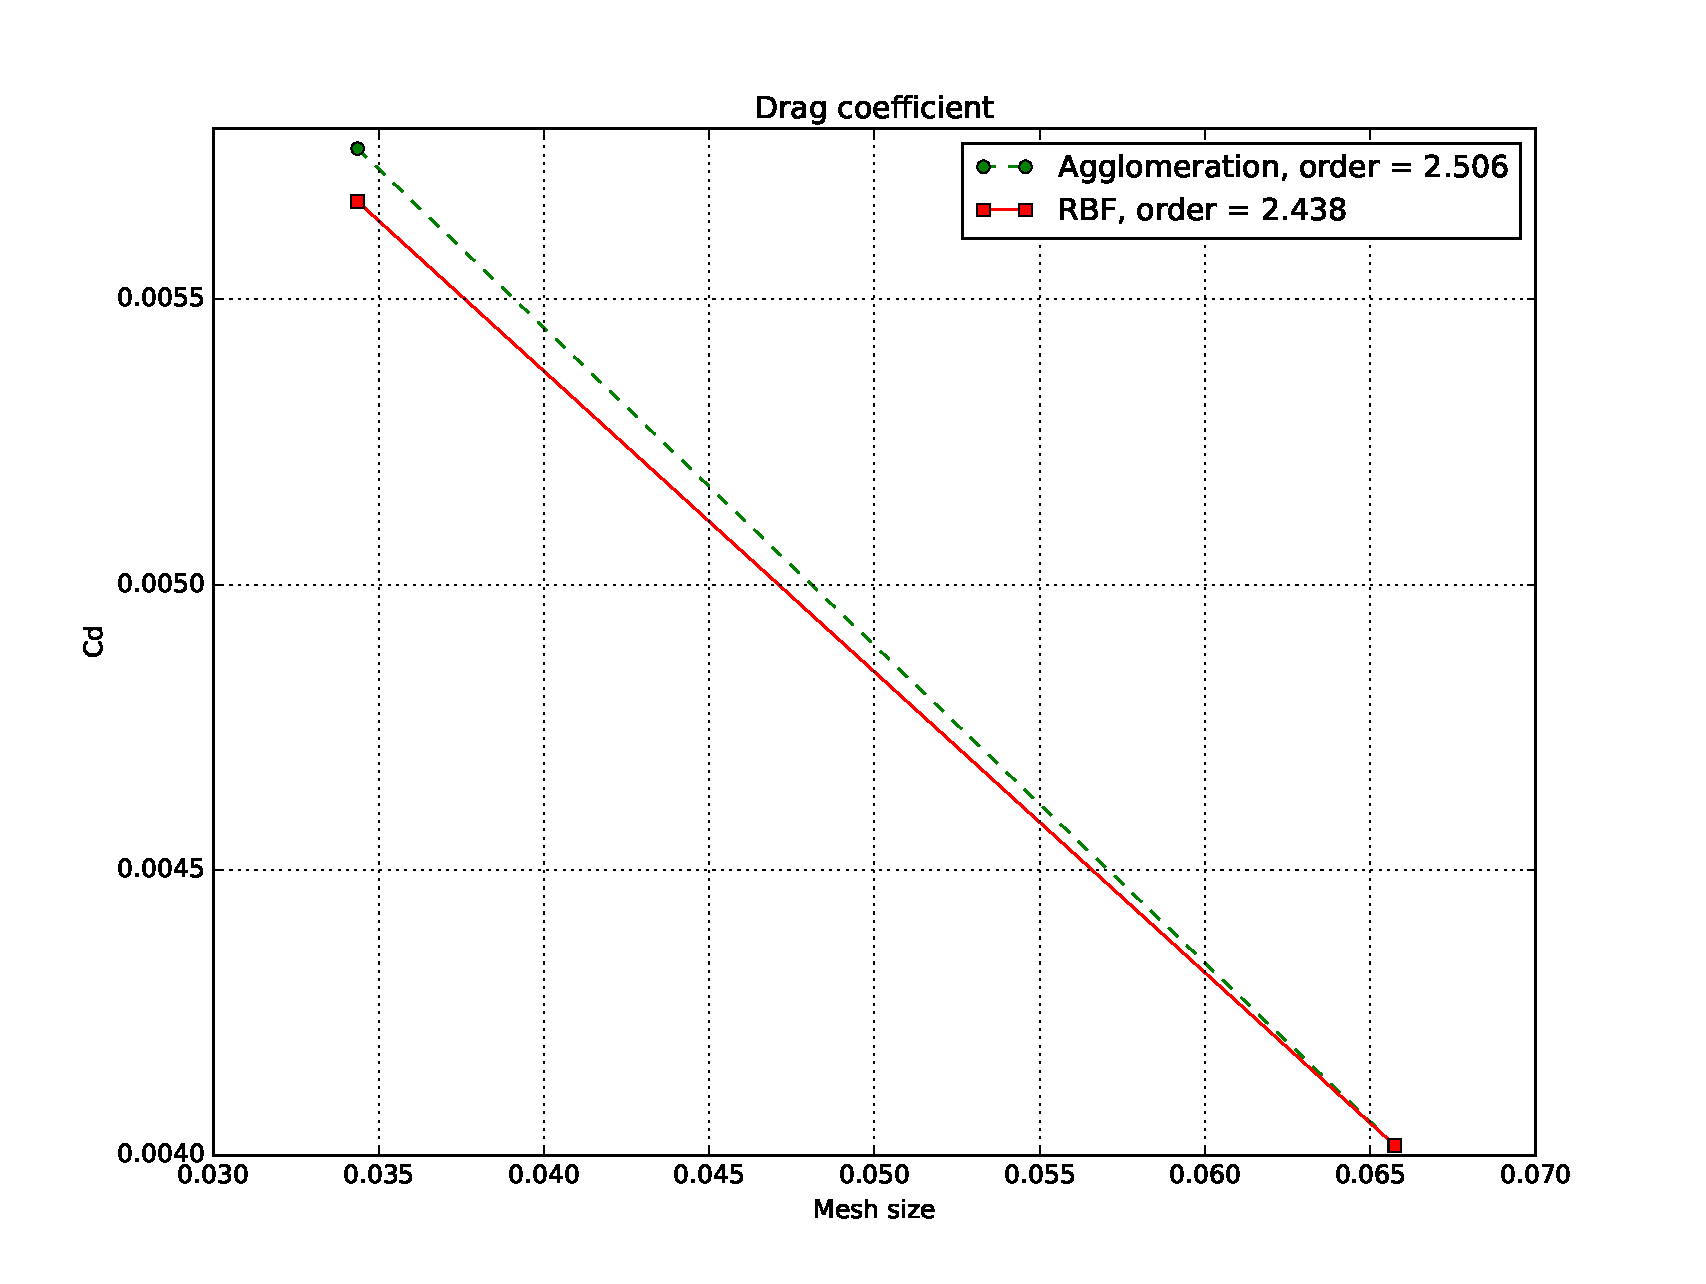
\includegraphics[scale=0.27]{cd_grid_conv}
	\caption{Accuracy (grid-convergence) of the solver using the agglomerated and RBF-curved mesh; the reference solution \cite{case:bump3d} is 0.0035897}
	\label{fig:gridconvergence}
\end{figure}
\end{frame}

\section{Conclusion}
\begin{frame}[allowframebreaks]{Conclusions - general mesh movement}
\begin{itemize}
\item Interpolation methods are generally well-suited for unsteady simulations that require mesh movement, as they are very fast.
\item When deformations are relatively small and not highly rotational, Delaunay graph mapping (DGM) is a good choice.
\item When larger and more general deformations are needed, the pure radial basis function (RBF) and to some extent the DGM with RBF interpolation (DGRBF) methods are good. 
\item The pure RBF method, while usually giving good robust results, is more expensive than the other interpolation methods considered here. The DGRBF methods, while being inexpensive, are only robust when implemented with angle interpolation (may be difficult to do for general mesh movements).
\item While linear elasticity methods generally perform well for mesh movement, they are much more expensive than the other methods and probably too expensive to use in unsteady simulations.
\end{itemize}
\end{frame}
\begin{frame}{Conclusions - curved mesh generation}
\begin{itemize}
	\item We find that RBF method is much more cost-effective than Jacobian-stiffened linear elasticity method for comparable results
	\item Both methods provide `knobs' to tune, such as the basis function and support radius in case of RBF and the stiffening criterion and stiffening exponent for the linear elasticity method
	\item Delaunay graph mapping methods, in their current state, are generally unusable for curved mesh generation.
\end{itemize}
\end{frame}
\begin{frame}{Future Directions}
\begin{itemize}
	\item Surface reconstruction in 3D - started, currently works only for smooth meshes. The technique used is `Weighted averaging of local fittings' \footfullcite{sr:jiaowang}. 
	Need detection of various kinds of singularities (`$C^1$ discontinuities') in the surface mesh.
	\item Automatic estimation of support radius for curved mesh generation by RBF; could try this based on local curvature estimates and density of interior mesh points nearby.
\end{itemize}
\end{frame}

\begin{frame}{Conference paper}
	A. Kashi and H. Luo. "Curved mesh generation using radial basis functions". In: AIAA AVIATION, June 2016. 
	
	(\emph{accepted})
\end{frame}

\printbibliography

\begin{frame}{RBF interpolation}
	Catch: The condition number of the left hand side scales as
	\begin{equation}
	\begin{aligned}
	\text{cond}_2 (\bld{A}) &= \mathcal{O}(q^{-5}) \quad \text{in 2D, and} \\
	\text{cond}_2 (\bld{A}) &= \mathcal{O}(q^{-6}) \quad \text{in 3D}
	\end{aligned}
	\end{equation}
	where
	\begin{equation}
	q := \min_{i\neq j} \lVert \bld{x}_{bi} - \bld{x}_{bj} \rVert_2
	\end{equation}
	is the minimum distance between any two boundary nodes.
	
	Iterative solvers do not always work! Sparse direct solvers are found to be a robust option.
\end{frame}

\end{document}
